%%%%%%%%%%%%%%%%%%%%%%%%%%%%% Thesis.tex %%%%%%%%%%%%%%%%%%%%%%%%%%%%%%%
%                                                                      %
%  ---------- Master of Science Dissertation template ----------       %
%                                                                      %
%  Template for the Master Thesis according to the regulations         %
%  published by the Academic Board (Direcção Académica) at IST.        %
%                                                                      %
%  For up-to-date guide, please refer to the offical website           %
%  http://da.tecnico.ulisboa.pt/dissertacao-de-mestrado/               %
%                                                                      %
%       Andre C. Marta                                                 %
%       Area Cientifica de Mecanica Aplicada e Aeroespacial            %
%       Departamento de Engenharia Mecanica                            %
%       Instituto Superior Tecnico                                     %
%       Av. Rovisco Pais                                               %
%       1049-001 Lisboa                                                %
%       Portugal                                                       %
%       Tel: +351 21 841 9469                                          %
%                        3469 (extension)                              %
%       Email: andre.marta@tecnico.ulisboa.pt                          %
%                                                                      %
%  Created:       Jan 20, 2011                                         %
%  Last Modified: Jul  2, 2015                                         %
%                                                                      %
%%%%%%%%%%%%%%%%%%%%%%%%%%%%%%%%%%%%%%%%%%%%%%%%%%%%%%%%%%%%%%%%%%%%%%%%
%  Revision history                                                    %
%  v1 - 2011/01/24 - original template                                 %
%  v2 - 2012/10/30 - new IST image and glossary support                %
%  v3 - 2013/12/10 - update according to 2012/13 official guide        %
%  v4 - 2014/02/28 - new default for bibliography style                %
%  v5 - 2014/05/07 - update according to 2013/14 official guide        %
%  v6 - 2015/07/02 - cover page format fixed,                          %
%                    contents page numbering fixed,                    %
%                    better language support,                          %
%                    enhanced examples of tables,                      %
%                    new option for appendix page numbering format,    %
%                    custom bibliography style                         %
%%%%%%%%%%%%%%%%%%%%%%%%%%%%%%%%%%%%%%%%%%%%%%%%%%%%%%%%%%%%%%%%%%%%%%%%
%                                                                      %
% To generate the PDF file, type "make" at the terminal prompt.        %
%                                                                      %
% The IST template LaTeX package was created by the author             %
% and it can be downloaded from:                                       %
% https://fenix.ist.utl.pt/homepage/ist31052/                          %
%                                                                      %
% The external packages can be downloaded from                         %
% the Comprehensive TeX Archive Network at http://www.ctan.org/        %
%                                                                      %
% List of LaTex symbols:                                               %
% http://www.ctan.org/tex-archive/info/symbols/comprehensive/          %
%                                                                      %
% Help with LaTex can be found at                                      %
% http://www.giss.nasa.gov/tools/latex/ltx-2.html                      %
% http://en.wikibooks.org/wiki/LaTeX                                   %
%%%%%%%%%%%%%%%%%%%%%%%%%%%%%%%%%%%%%%%%%%%%%%%%%%%%%%%%%%%%%%%%%%%%%%%%

%%%%%%%%%%%%%%%%%%%%%%%%%%%%%%%%%%%%%%%%%%%%%%%%%%%%%%%%%%%%%%%%%%%%%%%%
%     Preamble                                                         %
%%%%%%%%%%%%%%%%%%%%%%%%%%%%%%%%%%%%%%%%%%%%%%%%%%%%%%%%%%%%%%%%%%%%%%%%

% ----------------------------------------------------------------------
%  Set the document class
% ----------------------------------------------------------------------
\documentclass[10pt,a4paper,twoside]{report}

% ----------------------------------------------------------------------
% Define external packages, language, margins, fonts and new commands
% ----------------------------------------------------------------------
%%%%%%%%%%%%%%%%%%%%%%%%%%%%%%%%%%%%%%%%%%%%%%%%%%%%%%%%%%%%%%%%%%%%%%%%
%                                                                      %
%     File: Thesis_Preamble.tex                                        %
%     Tex Master: Thesis.tex                                           %
%                                                                      %
%     Author: Andre C. Marta                                           %
%     Last modified : 9 Apr 2015                                       %
%                                                                      %
%%%%%%%%%%%%%%%%%%%%%%%%%%%%%%%%%%%%%%%%%%%%%%%%%%%%%%%%%%%%%%%%%%%%%%%%

% ----------------------------------------------------------------------
% Define document language.
% ----------------------------------------------------------------------

% 'inputenc' package
%
% Accept different input encodings.
% http://www.ctan.org/tex-archive/macros/latex/base/
%
% > allows typing non-english text in LaTeX sources.
%
% ******************************* SELECT *******************************
%\usepackage[latin1]{inputenc} % <<<<< Windows
\usepackage[utf8]{inputenc}   % <<<<< Linux
% ******************************* SELECT *******************************


% 'babel' package
%
% Multilingual support for Plain TeX or LaTeX.
% http://www.ctan.org/tex-archive/macros/latex/required/babel/
%
% > sets the variable names according to the language selected
%
% ******************************* SELECT *******************************
%\usepackage[portuguese]{babel} % <<<<< Portuguese
\usepackage[english]{babel} % <<<<< English
% ******************************* SELECT *******************************


% List of LaTeX variable names: \abstractname, \appendixname, \bibname,
%   \chaptername, \contentsname, \listfigurename, \listtablename, ...)
% http://www.tex.ac.uk/cgi-bin/texfaq2html?label=fixnam
%
% Changing the words babel uses (uncomment and redefine as necessary...)
%
\newcommand{\acknowledgments}{@undefined} % new LaTeX variable name
%
% > English
%
\addto\captionsenglish{\renewcommand{\acknowledgments}{Acknowledgments}}
%\addto\captionsenglish{\renewcommand{\contentsname}{Contents}}
%\addto\captionsenglish{\renewcommand{\listtablename}{List of Tables}}
%\addto\captionsenglish{\renewcommand{\listfigurename}{List of Figures}}
%\addto\captionsenglish{\renewcommand{\nomname}{Nomenclature}}
%\addto\captionsenglish{\renewcommand{\glossaryname}{Glossary}}
%\addto\captionsenglish{\renewcommand{\acronymname}{List of Acronyms}}
%\addto\captionsenglish{\renewcommand{\bibname}{References}} % Bibliography
%\addto\captionsenglish{\renewcommand{\appendixname}{Appendix}}

% > Portuguese
%
\addto\captionsportuguese{\renewcommand{\acknowledgments}{Agradecimentos}}
%\addto\captionsportuguese{\renewcommand{\contentsname}{Conte\'{u}do}}
%\addto\captionsportuguese{\renewcommand{\listtablename}{Lista de Figuras}}
%\addto\captionsportuguese{\renewcommand{\listfigurename}{Lista de Tabelas}}
\addto\captionsportuguese{\renewcommand{\nomname}{Lista de S\'{i}mbolos}} % Nomenclatura
%\addto\captionsportuguese{\renewcommand{\glossary}{Gloss\'{a}rio}}
%\addto\captionsportuguese{\renewcommand{\acronymname}{Lista de Abrevia\c{c}\~{o}es}}
%\addto\captionsportuguese{\renewcommand{\bibname}{Refer\^{e}ncias}} % Bibliografia
%\addto\captionsportuguese{\renewcommand{\appendixname}{Anexo}} % Apendice


% ----------------------------------------------------------------------
% Define cover fields in both english and portuguese.
% ----------------------------------------------------------------------
%
\newcommand{\coverThesis}{@undefined} % new LaTeX variable name
\newcommand{\coverSupervisors}{@undefined} % new LaTeX variable name
\newcommand{\coverExaminationCommittee}{@undefined} % new LaTeX variable name
\newcommand{\coverChairperson}{@undefined} % new LaTeX variable name
\newcommand{\coverSupervisor}{@undefined} % new LaTeX variable name
\newcommand{\coverMemberCommittee}{@undefined} % new LaTeX variable name
% > English
\addto\captionsenglish{\renewcommand{\coverThesis}{Thesis to obtain the Master of Science Degree in}}
\addto\captionsenglish{\renewcommand{\coverSupervisors}{Supervisor(s)}}
\addto\captionsenglish{\renewcommand{\coverExaminationCommittee}{Examination Committee}}
\addto\captionsenglish{\renewcommand{\coverChairperson}{Chairperson}}
\addto\captionsenglish{\renewcommand{\coverSupervisor}{Supervisor}}
\addto\captionsenglish{\renewcommand{\coverMemberCommittee}{Member of the Committee}}
% > Portuguese
\addto\captionsportuguese{\renewcommand{\coverThesis}{Disserta\c{c}\~{a}o para obten\c{c}\~{a}o do Grau de Mestre em}}
\addto\captionsportuguese{\renewcommand{\coverSupervisors}{Orientador(es)}}
\addto\captionsportuguese{\renewcommand{\coverExaminationCommittee}{J\'{u}ri}}
\addto\captionsportuguese{\renewcommand{\coverChairperson}{Presidente}}
\addto\captionsportuguese{\renewcommand{\coverSupervisor}{Orientador}}
\addto\captionsportuguese{\renewcommand{\coverMemberCommittee}{Vogal}}


% ----------------------------------------------------------------------
% Define default and cover page fonts.
% ----------------------------------------------------------------------

% Use Arial font as default
%
\renewcommand{\rmdefault}{phv}
\renewcommand{\sfdefault}{phv}

% Define cover page fonts
%
%         encoding     family       series      shape
%  \usefont{T1}     {phv}=helvetica  {b}=bold    {n}=normal
%                   {ptm}=times      {m}=normal  {sl}=slanted
%                                                {it}=italic
% see more examples at
% http://julien.coron.free.fr/languages/latex/fonts/
%
\def\FontLn{% 16 pt normal
  \usefont{T1}{phv}{m}{n}\fontsize{16pt}{16pt}\selectfont}
\def\FontLb{% 16 pt bold
  \usefont{T1}{phv}{b}{n}\fontsize{16pt}{16pt}\selectfont}
\def\FontMn{% 14 pt normal
  \usefont{T1}{phv}{m}{n}\fontsize{14pt}{14pt}\selectfont}
\def\FontMb{% 14 pt bold
  \usefont{T1}{phv}{b}{n}\fontsize{14pt}{14pt}\selectfont}
\def\FontSn{% 12 pt normal
  \usefont{T1}{phv}{m}{n}\fontsize{12pt}{12pt}\selectfont}


% ----------------------------------------------------------------------
% Define page margins and line spacing.
% ----------------------------------------------------------------------

% 'geometry' package
%
% Flexible and complete interface to document dimensions.
% http://www.ctan.org/tex-archive/macros/latex/contrib/geometry/
%
% > set the page margins (2.5cm minimum in every side, as per IST rules)
%
\usepackage{geometry}	
\geometry{verbose,tmargin=2.5cm,bmargin=2.5cm,lmargin=2.5cm,rmargin=2.5cm}

% 'setspace' package
%
% Set space between lines.
% http://www.ctan.org/tex-archive/macros/latex/contrib/setspace/
%
% > allow setting line spacing (line spacing of 1.5, as per IST rules)
%
\usepackage{setspace}
\renewcommand{\baselinestretch}{1.5}


% ----------------------------------------------------------------------
% Include external packages.
% Note that not all of these packages may be available on all system
% installations. If necessary, include the .sty files locally in
% the <jobname>.tex file directory.
% ----------------------------------------------------------------------

% 'graphicx' package
%
% Enhanced support for graphics.
% http://www.ctan.org/tex-archive/macros/latex/required/graphics/
%
% > extends arguments of the \includegraphics command
%
\usepackage{graphicx}


% 'color' package
%
% Colour control for LaTeX documents.
% http://www.ctan.org/tex-archive/macros/latex/required/graphics/
%
% > defines color macros: \color{<color name>}
%
%\usepackage{color}


% 'amsmath' package
%
% Mathematical enhancements for LaTeX.
% http://www.ctan.org/tex-archive/macros/latex/required/amslatex/
%
% > American Mathematical Society plain Tex macros
%
\usepackage{amsmath}  % AMS mathematical facilities for LaTeX.
\usepackage{amsthm}   % Typesetting theorems (AMS style).
\usepackage{amsfonts} % 


% 'wrapfig' package
%
% Produces figures which text can flow around.
% http://www.ctan.org/tex-archive/macros/latex/contrib/wrapfig/
%
% > wrap figures/tables in text (i.e., Di Vinci style)
%
% \usepackage{wrapfig}


% 'subfigure' package
%
% Deprecated: Figures divided into subfigures.
% http://www.ctan.org/tex-archive/obsolete/macros/latex/contrib/subfigure/
%
% > subcaptions for subfigures
%
\usepackage{subfigure}


% 'subfigmat' package
%
% Automates layout when using the subfigure package.
% http://www.ctan.org/tex-archive/macros/latex/contrib/subfigmat/
%
% > matrices of similar subfigures
%
\usepackage{subfigmat}


% 'url' package
%
% Verbatim with URL-sensitive line breaks.
% http://www.ctan.org/tex-archive/macros/latex/contrib/url/
%
% > URLs in BibTex
%
% \usepackage{url}


% 'varioref' package
%
% Intelligent page references.
% http://www.ctan.org/tex-archive/macros/latex/required/tools/
%
% > smart page, figure, table and equation referencing
%
%\usepackage{varioref}


% 'dcolumn' package
%
% Align on the decimal point of numbers in tabular columns.
% http://www.ctan.org/tex-archive/macros/latex/required/tools/
%
% > decimal-aligned tabular math columns
%
\usepackage{dcolumn}
\newcolumntype{d}{D{.}{.}{-1}} % column aligned by the point separator '.'
\newcolumntype{e}{D{E}{E}{-1}} % column aligned by the exponent 'E'


% '' package
%
% Reimplementation of and extensions to LaTeX verbatim.
% http://www.ctan.org/tex-archive/macros/latex/required/tools/
%
% > provides the verbatim environment (\begin{verbatim},\end{verbatim})
%   and a comment environment (\begin{comment},  \end{comment})
%
% \usepackage{verbatim}


% 'moreverb' package
%
% Extended verbatim.
% http://www.ctan.org/tex-archive/macros/latex/contrib/moreverb/
%
% > supports tab expansion and line numbering
%
% \usepackage{moreverb}



% 'nomencl' package
%
% Produce lists of symbols as in nomenclature.
% http://www.ctan.org/tex-archive/macros/latex/contrib/nomencl/
%
% The nomencl package makes use of the MakeIndex program
% in order to produce the nomenclature list.
%
% Nomenclature
% 1) On running the file through LATEX, the command \makenomenclature
%    in the preamble instructs it to create/open the nomenclature file
%    <jobname>.nlo corresponding to the LATEX file <jobname>.tex and
%    writes the information from the \nomenclature commands to this file.
% 2) The next step is to invoke MakeIndex in order to produce the
%    <jobname>.nls file. This can be achieved by making use of the
%    command: makeindex <jobname>.nlo -s nomencl.ist -o <jobname>.nls
% 3) The last step is to invoke LATEX on the <jobname>.tex file once
%    more. There, the \printnomenclature in the document will input the
%    <jobname>.nls file and process it according to the given options.
%
% http://www-h.eng.cam.ac.uk/help/tpl/textprocessing/nomencl.pdf
%
% Nomenclature (produces *.nlo *.nls files)
\usepackage{nomencl}
\makenomenclature
%
% Group variables according to their symbol type
%
\RequirePackage{ifthen} 
\ifthenelse{\equal{\languagename}{english}}%
    { % English
    \renewcommand{\nomgroup}[1]{%
      \ifthenelse{\equal{#1}{R}}{%
        \item[\textbf{Roman symbols}]}{%
        \ifthenelse{\equal{#1}{G}}{%
          \item[\textbf{Greek symbols}]}{%
          \ifthenelse{\equal{#1}{S}}{%
            \item[\textbf{Subscripts}]}{%
            \ifthenelse{\equal{#1}{T}}{%
              \item[\textbf{Superscripts}]}{}}}}}%
    }{% Portuguese
    \renewcommand{\nomgroup}[1]{%
      \ifthenelse{\equal{#1}{R}}{%
        \item[\textbf{Simbolos romanos}]}{%
        \ifthenelse{\equal{#1}{G}}{%
          \item[\textbf{Simbolos gregos}]}{%
          \ifthenelse{\equal{#1}{S}}{%
            \item[\textbf{Subscritos}]}{%
            \ifthenelse{\equal{#1}{T}}{%
              \item[\textbf{Sobrescritos}]}{}}}}}%
    }%


% 'glossary' package
%
% Create a glossary.
% http://www.ctan.org/tex-archive/macros/latex/contrib/glossary/
%
% Glossary (produces *.glo *.ist files)
\usepackage[number=none]{glossary}
% (remove blank line between groups)
\setglossary{gloskip={}}
% (redefine glossary style file)
%\renewcommand{\istfilename}{myGlossaryStyle.ist}
\makeglossary


% 'rotating' package
%
% Rotation tools, including rotated full-page floats.
% http://www.ctan.org/tex-archive/macros/latex/contrib/rotating/
%
% > show wide figures and tables in landscape format:
%   use \begin{sidewaystable} and \begin{sidewaysfigure}
%   instead of 'table' and 'figure', respectively.
%
\usepackage{rotating}


% 'hyperref' package
%
% Extensive support for hypertext in LaTeX.
% http://www.ctan.org/tex-archive/macros/latex/contrib/hyperref/
%
% > Extends the functionality of all the LATEX cross-referencing
%   commands (including the table of contents, bibliographies etc) to
%   produce \special commands which a driver can turn into hypertext
%   links; Also provides new commands to allow the user to write adhoc
%   hypertext links, including those to external documents and URLs.
%
\usepackage[pdftex]{hyperref} % enhance documents that are to be
                              % output as HTML and PDF
\hypersetup{colorlinks,       % color text of links and anchors,
                              % eliminates borders around links
%            linkcolor=red,    % color for normal internal links
            linkcolor=black,  % color for normal internal links
            anchorcolor=black,% color for anchor text
%            citecolor=green,  % color for bibliographical citations
            citecolor=black,  % color for bibliographical citations
%            filecolor=magenta,% color for URLs which open local files
            filecolor=black,  % color for URLs which open local files
%            menucolor=red,    % color for Acrobat menu items
            menucolor=black,  % color for Acrobat menu items
%            pagecolor=red,    % color for links to other pages
            pagecolor=black,  % color for links to other pages
%            urlcolor=cyan,    % color for linked URLs
            urlcolor=black,   % color for linked URLs
	          bookmarks=true,         % create PDF bookmarks
	          bookmarksopen=false,    % don't expand bookmarks
	          bookmarksnumbered=true, % number bookmarks
	          pdftitle={Thesis},
            pdfauthor={Andre C. Marta},
            pdfsubject={Thesis Title},
            pdfkeywords={Thesis Keywords},
            pdfstartview=FitV,
            pdfdisplaydoctitle=true}


% 'hypcap' package
%
% Adjusting the anchors of captions.
% http://www.ctan.org/tex-archive/macros/latex/contrib/oberdiek/
%
% > fixes the problem with hyperref, that links to floats points
%   below the caption and not at the beginning of the float.
%
\usepackage[figure,table]{hypcap}


% 'natbib' package
%
% Flexible bibliography support.
% http://www.ctan.org/tex-archive/macros/latex/contrib/natbib/
%
% > produce author-year style citations
%
% \citet  and \citep  for textual and parenthetical citations, respectively
% \citet* and \citep* that print the full author list, and not just the abbreviated one
% \citealt is the same as \citet but without parentheses. Similarly, \citealp is \citep without parentheses
% \citeauthor
% \citeyear
% \citeyearpar
%
% ******************************* SELECT *******************************
%\usepackage{natbib}          % <<<<< References in alphabetical list Correia, Silva, ...
\usepackage[numbers]{natbib} % <<<<< References in numbered list [1],[2],...
% ******************************* SELECT *******************************


% 'notoccite' package
%
% Prevent trouble from citations in table of contents, etc.
% http://ctan.org/pkg/notoccite
%
% > If you have \cite com­mands in \sec­tion-like com­mands, or in \cap­tion,
%   the ci­ta­tion will also ap­pear in the ta­ble of con­tents, or list of what­ever.
%   If you are also us­ing an un­srt-like bib­li­og­ra­phy style, these ci­ta­tions will
%   come at the very start of the bib­li­og­ra­phy, which is con­fus­ing. This pack­age
%   sup­presses the ef­fect.
%
\usepackage{notoccite}


% 'multirow' package
%
% Create tabular cells spanning multiple rows
% http://www.ctan.org/pkg/multirow
%
\usepackage{multirow}


% 'booktabs' package
%
% Publication quality tables in LaTeX
% http://www.ctan.org/pkg/booktabs
%
% > en­hance the qual­ity of ta­bles in LaTeX, pro­vid­ing ex­tra com­mands.
%
% \renewcommand{\arraystretch}{<ratio>} % space between rows
%
\usepackage{booktabs}
%\newcommand{\ra}[1]{\renewcommand{\arraystretch}{#1}}


% 'pdfpages' package
%
% Include PDF documents in LaTeX
% http://www.ctan.org/pkg/pdfpages
%
% > in­clu­sion of ex­ter­nal multi-page PDF doc­u­ments in LaTeX doc­u­ments.
%   Pages may be freely se­lected and sim­i­lar to psnup it is pos­si­ble to put
%   sev­eral log­i­cal pages onto each sheet of pa­per.
%
% \includepdf{filename.pdf}
% \includepdf[pages={4-9},nup=2x3,landscape=true]{filename.pdf}
%
\usepackage{pdfpages}


% ----------------------------------------------------------------------
% Define new commands to assure consistent treatment throughout document
% ----------------------------------------------------------------------

\newcommand{\ud}{\mathrm{d}}                % total derivative
\newcommand{\degree}{\ensuremath{^\circ\,}} % degrees

% Abbreviations

\newcommand{\mcol}{\multicolumn}            % table format

\newcommand{\eqnref}[1]{(\ref{#1})}
\newcommand{\class}[1]{\texttt{#1}}
\newcommand{\package}[1]{\texttt{#1}}
\newcommand{\file}[1]{\texttt{#1}}
\newcommand{\BibTeX}{\textsc{Bib}\TeX}

% Typefaces ( example: {\bf Bold text here} )
%
% > pre-defined
%   \bf % bold face
%   \it % italic
%   \tt % typewriter
%
% > newly defined
\newcommand{\tr}[1]{{\ensuremath{\textrm{#1}}}}   % text roman
\newcommand{\tb}[1]{{\ensuremath{\textbf{#1}}}}   % text bold face
\newcommand{\ti}[1]{{\ensuremath{\textit{#1}}}}   % text italic
\newcommand{\mc}[1]{{\ensuremath{\mathcal{#1}}}}  % math calygraphy
\newcommand{\mco}[1]{{\ensuremath{\mathcalold{#1}}}}% math old calygraphy
\newcommand{\mr}[1]{{\ensuremath{\mathrm{#1}}}}   % math roman
\newcommand{\mb}[1]{{\ensuremath{\mathbf{#1}}}}   % math bold face
\newcommand{\bs}[1]{\ensuremath{\boldsymbol{#1}}} % math symbol
\def\bm#1{\mathchoice                             % math bold
  {\mbox{\boldmath$\displaystyle#1$}}%
  {\mbox{\boldmath$#1$}}%
  {\mbox{\boldmath$\scriptstyle#1$}}%
  {\mbox{\boldmath$\scriptscriptstyle#1$}}}
\newcommand{\boldcal}[1]{{\ensuremath{\boldsymbol{\mathcal{#1}}}}}% math bold calygraphy

 % file "Thesis_Preamble.tex"

%%%%%%%%%%%%%%%%%%%%%%%%%%%%%%%%%%%%%%%%%%%%%%%%%%%%%%%%%%%%%%%%%%%%%%%%
%     Begin Document                                                   %
%%%%%%%%%%%%%%%%%%%%%%%%%%%%%%%%%%%%%%%%%%%%%%%%%%%%%%%%%%%%%%%%%%%%%%%%
\begin{document}

% Set plain page style (no headers, footer with centered page number)
\pagestyle{plain}

% Set roman numbering (i,ii,...) before the start of chapters
\pagenumbering{roman}

% ----------------------------------------------------------------------
%  Cover page
% ----------------------------------------------------------------------
%%%%%%%%%%%%%%%%%%%%%%%%%%%%%%%%%%%%%%%%%%%%%%%%%%%%%%%%%%%%%%%%%%%%%%%%
%                                                                      %
%     File: Thesis_FrontCover.tex                                      %
%     Tex Master: Thesis.tex                                           %
%                                                                      %
%     Author: Andre C. Marta                                           %
%     Last modified :  2 Jul 2015                                      %
%                                                                      %
%%%%%%%%%%%%%%%%%%%%%%%%%%%%%%%%%%%%%%%%%%%%%%%%%%%%%%%%%%%%%%%%%%%%%%%%

\thispagestyle {empty}

% IST Logo - Signature A
% parameters: bb=llx lly urx ury (bounding box), width=h_length, height=v_length, angle=angle, scale=factor, clip=true/false, draft=true/false. 

\includegraphics[bb=9.5cm 11cm 0cm 0cm,scale=0.29]{IST_A_CMYK_POS}

\begin{center}
%
% Figure (Image or plot)
\vspace{2.5cm}
% height = 50 mm


% Title, author and degree
\vspace{1.0cm}
{\FontLb Nonlinear Control Applied to 4D Transport Aircraft Guidance}\\ % <<<<< EDIT TITLE
%\vspace{0.2cm}
%{\FontMn Subtitle (optional)} \\
%\vspace{1.9cm}
\vspace{2.6cm}
{\FontMb Guilherme Goulão de Sousa} \\ % <<<<< EDIT NAME
\vspace{2.0cm}
{\FontSn \coverThesis} \\
\vspace{0.3cm}
{\FontLb Aerospace Engineering} \\ % <<<<< EDIT COURSE
\vspace{1.0cm}
{\FontSn %
\begin{tabular}{ll}
 \coverSupervisors: & Prof. José Raul Azinheira \\ % <<<<< EDIT NAME
                    & Prof. Felix Mora-Camino    % <<<<< EDIT NAME
\end{tabular} } \\
\vspace{1.0cm}
{\FontMb \coverExaminationCommittee} \\
\vspace{0.3cm}
{\FontSn %
\begin{tabular}{c}
\coverChairperson:     Prof. Full Name          \\ % <<<<< EDIT NAME
\coverSupervisor:      Prof. Full Name 1 (or 2) \\ % <<<<< EDIT NAME
\coverMemberCommittee: Prof. Full Name 3           % <<<<< EDIT NAME
\end{tabular} } \\
\vspace{1.5cm}
{\FontMb November 2017} \\ % <<<<< EDIT DATE (corresponds to date of oral examination)
%
\end{center}

 % file "Thesis_FrontCover.tex"
\cleardoublepage

% ----------------------------------------------------------------------
% Dedication page (optional)
% ----------------------------------------------------------------------
%%%%%%%%%%%%%%%%%%%%%%%%%%%%%%%%%%%%%%%%%%%%%%%%%%%%%%%%%%%%%%%%%%%%%%%%
%                                                                      %
%     File: Thesis_Dedication.tex                                      %
%     Tex Master: Thesis.tex                                           %
%                                                                      %
%     Author: Andre C. Marta                                           %
%     Last modified :  2 Jul 2015                                      %
%                                                                      %
%%%%%%%%%%%%%%%%%%%%%%%%%%%%%%%%%%%%%%%%%%%%%%%%%%%%%%%%%%%%%%%%%%%%%%%%

\null\vskip5cm%
\begin{flushright}
     Dedicated to someone special...
\end{flushright}
\vfill\newpage

 % file "Thesis_Dedication.tex"
\cleardoublepage

% ----------------------------------------------------------------------
%  Acknowledgments (optional)
% ----------------------------------------------------------------------
%%%%%%%%%%%%%%%%%%%%%%%%%%%%%%%%%%%%%%%%%%%%%%%%%%%%%%%%%%%%%%%%%%%%%%%%
%                                                                      %
%     File: Thesis_Acknowledgments.tex                                 %
%     Tex Master: Thesis.tex                                           %
%                                                                      %
%     Author: Andre C. Marta                                           %
%     Last modified :  2 Jul 2015                                      %
%                                                                      %
%%%%%%%%%%%%%%%%%%%%%%%%%%%%%%%%%%%%%%%%%%%%%%%%%%%%%%%%%%%%%%%%%%%%%%%%

\section*{\acknowledgments}

% Add entry in the table of contents as section
\addcontentsline{toc}{section}{\acknowledgments}
{\setlength{\parindent}{0cm}
I would like first of all to thank my family, for giving me more love and support all the way through writing this thesis that I could ever ask for.


To B., for being an amazing person and always being there for me during for the hardships.


To Prof. Azinheira, for his thoroughness that immensely helped improve the quality of this work.

To Hector Escamilla, for being a great mentor and a better guide through these six months of work.

I would also like to thank the ERASMUS Placement programme, for allowing me and many other students to have such an enriching experience abroad.}

 % file "Thesis_Acknowledgements.tex"
\cleardoublepage

% ----------------------------------------------------------------------
%  Abstract (both in English and Portuguese)
% ----------------------------------------------------------------------
%%%%%%%%%%%%%%%%%%%%%%%%%%%%%%%%%%%%%%%%%%%%%%%%%%%%%%%%%%%%%%%%%%%%%%%%
%                                                                      %
%     File: Thesis_Resumo.tex                                          %
%     Tex Master: Thesis.tex                                           %
%                                                                      %
%     Author: Andre C. Marta                                           %
%     Last modified :  2 Jul 2015                                      %
%                                                                      %
%%%%%%%%%%%%%%%%%%%%%%%%%%%%%%%%%%%%%%%%%%%%%%%%%%%%%%%%%%%%%%%%%%%%%%%%

\section*{Resumo}

% Add entry in the table of contents as section
\addcontentsline{toc}{section}{Resumo}

Seguindo a mudança de paradigma que acontece atualmente da industria do tráfego aéro, esta tese de mestrado propõe um controlador para aviões comerciais permitindo o seguimento de trajectórias 4D, aumentando assim a segurança e capacidade num dado espaço aéro. A lei de controlo utilizada é baseada no método de linearização por feedback, e uma rede neural é também implementada de modo a reduzir os erros causados por incertezas na modelização do sistema, causados por erros de estimação dos parâmetros do avião, perturbações externas ou até falhas de systema. A rede neural é treinada online, utilizando o algoritmo de retro-propagação, de modo a otimizar a inversão não-linear, resultando assim num controlador adaptivo. Os resultados de simulações mostram que este controlador é capaz de manter o sistema estável e controlável em condições em que tal não é possível.

\vfill

\textbf{\Large Palavras-chave:} controlo não linear, linearização por feedback, rede neural, controlo de voo, back-propagation

   % file "Thesis_Resumo.tex"
\cleardoublepage

%%%%%%%%%%%%%%%%%%%%%%%%%%%%%%%%%%%%%%%%%%%%%%%%%%%%%%%%%%%%%%%%%%%%%%%%
%                                                                      %
%     File: Thesis_Abstract.tex                                        %
%     Tex Master: Thesis.tex                                           %
%                                                                      %
%     Author: Andre C. Marta                                           %
%     Last modified :  2 Jul 2015                                      %
%                                                                      %
%%%%%%%%%%%%%%%%%%%%%%%%%%%%%%%%%%%%%%%%%%%%%%%%%%%%%%%%%%%%%%%%%%%%%%%%

\section*{Abstract}

% Add entry in the table of contents as section
\addcontentsline{toc}{section}{Abstract}

Insert your abstract here with a maximum of 250 words, followed by 4 to 6 keywords...

\vfill

\textbf{\Large Keywords:} keyword1, keyword2,...

 % file "Thesis_Abstract.tex"
\cleardoublepage

% ----------------------------------------------------------------------
%  Table of contents, list of tables, list of figures and nomenclature
% ----------------------------------------------------------------------

% Table of contents
%
\tableofcontents
\cleardoublepage 

% List of tables
%
% Add entry in the table of contents as section
\phantomsection
\addcontentsline{toc}{section}{\listtablename}
% Generate list
\listoftables
\cleardoublepage 

% List of figures
%
% Add entry in the table of contents as section
\phantomsection
\addcontentsline{toc}{section}{\listfigurename}
% Generate list
\listoffigures
\cleardoublepage 

% Nomenclature
%
% entries of nomenclature list
%%%%%%%%%%%%%%%%%%%%%%%%%%%%%%%%%%%%%%%%%%%%%%%%%%%%%%%%%%%%%%%%%%%%%%%%
%                                                                      %
%     File: Thesis_Nomenclature.tex                                    %
%     Tex Master: Thesis.tex                                           %
%                                                                      %
%     Author: Andre C. Marta                                           %
%     Last modified : 21 Jan 2011                                      %
%                                                                      %
%%%%%%%%%%%%%%%%%%%%%%%%%%%%%%%%%%%%%%%%%%%%%%%%%%%%%%%%%%%%%%%%%%%%%%%%
%
% The definitions can be placed anywhere in the document body
% and their order is sorted by <symbol> automatically when
% calling makeindex in the makefile
%
% The \glossary command has the following syntax:
%
% \glossary{entry}
%
% The \nomenclature command has the following syntax:
%
% \nomenclature[<prefix>]{<symbol>}{<description>}
%
% where <prefix> is used for fine tuning the sort order,
% <symbol> is the symbol to be described, and <description> is
% the actual description.

% ----------------------------------------------------------------------

\nomenclature{NN}{Neural Network}
\nomenclature{FBL}{Feedback Linearisation}
\nomenclature{DI}{Dynamic Inversion}
\nomenclature{BP}{Backpropagation}
% Roman symbols [r]
\nomenclature[ru]{$\bf u$}{Velocity vector}
\nomenclature[ru]{$u,v,w$}{Velocity Cartesian components}
\nomenclature[r]{$p, q, r$}{Angular Velocity Cartesian components}
\nomenclature[rp]{$p$}{Pressure}
\nomenclature[rC]{$C_D$}{Coefficient of drag}
\nomenclature[rC]{$C_L$}{Coefficient of lift}
\nomenclature[rT]{$T$}{Thrust}
\nomenclature[rW]{$W$}{Weight}
\nomenclature[r]{$V_a$}{Airspeed}
% ----------------------------------------------------------------------
% Greek symbols [g]
\nomenclature[g]{$\rho$}{Density}
\nomenclature[g]{$\alpha$}{Angle of attack}
\nomenclature[g]{$\beta$}{Angle of side-slip}
\nomenclature[g]{$\Omega$}{Angular velocity vector}
\nomenclature[g]{$\phi,\theta, \psi$}{Pitch, Roll and Yaw Euler angles} % file "Thesis_Nomenclature.tex"
%
% Add entry in the table of contents as section
\phantomsection
\addcontentsline{toc}{section}{\nomname}
% Insert glossary/nomenclature section produced by MakeIndex
\printnomenclature
\cleardoublepage

% entries of glossary list
%%%%%%%%%%%%%%%%%%%%%%%%%%%%%%%%%%%%%%%%%%%%%%%%%%%%%%%%%%%%%%%%%%%%%%%%
%                                                                      %
%     File: Thesis_Glossary.tex                                        %
%     Tex Master: Thesis.tex                                           %
%                                                                      %
%     Author: Andre C. Marta                                           %
%     Last modified : 30 Oct 2012                                      %
%                                                                      %
%%%%%%%%%%%%%%%%%%%%%%%%%%%%%%%%%%%%%%%%%%%%%%%%%%%%%%%%%%%%%%%%%%%%%%%%
%
% The definitions can be placed anywhere in the document body
% and their order is sorted by <symbol> automatically when
% calling makeindex in the makefile
%
% The \glossary command has the following syntax:
%
% \glossary{entry}
%
% The \nomenclature command has the following syntax:
%
% \nomenclature[<prefix>]{<symbol>}{<description>}
%
% where <prefix> is used for fine tuning the sort order,
% <symbol> is the symbol to be described, and <description> is
% the actual description.

% ----------------------------------------------------------------------

\glossary{name={\textbf{MDO}},description={Multi-Disciplinar Optimization is an engineering technique that uses optimization methods to solve design problems incorporating two or more disciplines.}}

\glossary{name={\textbf{CFD}},description={Computational Fluid Dynamics is a branch of fluid mechanics that uses numerical methods and algorithms to solve problems that involve fluid flows.}}

\glossary{name={\textbf{CSM}},description={Computational Structural Mechanics is a branch of structure mechanics that uses numerical methods and algorithms to perform the analysis of structures and its components.}}

 % file "Thesis_Glossary.tex"

% Add entry in the table of contents as section
\phantomsection
\addcontentsline{toc}{section}{\glossaryname}
% Insert glossary section produced by MakeIndex
\printglossary
\cleardoublepage

% Set arabic numbering (1,2,...) after preface
%
\setcounter{page}{1}
\pagenumbering{arabic}

% ----------------------------------------------------------------------
%  Chapters
% ----------------------------------------------------------------------

%%%%%%%%%%%%%%%%%%%%%%%%%%%%%%%%%%%%%%%%%%%%%%%%%%%%%%%%%%%%%%%%%%%%%%%%
%                                                                      %
%     File: Thesis_Introduction.tex                                    %
%     Tex Master: Thesis.tex                                           %
%                                                                      %
%     Author: Andre C. Marta                                           %
%     Last modified :  2 Jul 2015                                      %
%                                                                      %
%%%%%%%%%%%%%%%%%%%%%%%%%%%%%%%%%%%%%%%%%%%%%%%%%%%%%%%%%%%%%%%%%%%%%%%%

\chapter{Introduction}
\label{chapter:introduction}


Due to their inherent non-linear dynamics, designing control systems for both rotary and fixed wing aircraft is a non-trivial task, where using linear control approaches reveal to be inaccurate. Feedback linearisation is an approach to non-linear control design that algebraically transforms a non-linear system into a linear one. For the linearised system linear control techniques can be used. Note that in this work other equivalent terms to feedback linearisation will be used, namely nonlinear inversion (NLI) and dynamic inversion. 
However this approach, as well as other state-of-the art control approaches such as model predictive control, backstepping and gain scheduling require the \textit{a priori} exact mathematical model of the system to be controlled \cite{SotA_IFCS}. The lack of such an exact model leads to errors in the calculation of the model inversion, necessary to implement feedback linearisation. Indeed, while feedback linearisation control shows good tracking, it is sensitive to parameter uncertainties, that ultimately lead to these inversion errors \cite{SotA_ControlAlgorithm}, and in extreme cases to instability. One solution to this problem that has gained momentum over the last years is the use augmentation algorithms, namely neural networks and other intelligent algorithms, to minimize and cancel the resulting guidance error\cite{NLI+NN}, \cite{NLI+NN_IFCS}, \cite{NLI+NN_chinese}. 

This paper aims to discuss the existing alternatives to augment the precision, robustness and overall performance of feedback linearisation control. A second goal of this work will be to extend the solutions used to increase the robustness of feedback linearisation control to provide an adaptive control in cases of system failures and strong external disturbances.



%%%%%%%%%%%%%%%%%%%%%%%%%%%%%%%%%%%%%%%%%%%%%%%%%%%%%%%%%%%%%%%%%%%%%%%%
\section{Motivation}
\label{section:motivation}

As the aeronautic industry grows, so is bound to also grow the air traffic dramatically. To answer this problematic, ATM researchers have proposed over the last few years Trajectory-Based Operations (TBO), a concept allowing the use of 4D trajectories to manage both safety and air capacity. In both the US and Europe, initiatives to put such systems in place are currently being developed and implemented, namely the NextGen by the FAA and SESAR EUROCONTROL. Therefore, in order to adopt this air traffic management paradigm, automation will play a crucial role in 4D guidance control, allowing an aircraft to follow flight plans more accurately.

%%%%%%%%%%%%%%%%%%%%%%%%%%%%%%%%%%%%%%%%%%%%%%%%%%%%%%%%%%%%%%%%%%%%%%%%
\section{Topic Overview}
\label{section:overview}

In order to fully automatize a commercial aircraft to follow a 4D trajectory in cruise conditions, this work will focus on designing and implementing an autopilot capable of controlling the aircraft attitude, improving flight quality and stability in hazardous piloting situations, to be integrated in a Fly-by-Wire system. The ultimate aim of this project will be to focus on auto pilot to provide 4D trajectory guidance to a commercial aircraft. To do so a model based controller is used, unlike in the currently implemented framework of robust control composed of several PID layers. This model based controller distinguishes fast and slow dynamics, using a nonlinear inversion of the fast dynamics to determine the necessary deflections of the control surfaces. Unlike PIDs and controllers that use linearisation through the Jacobian using Taylor series expansions of the nonlinear system, that may yield unsatisfactory performance and robustness at a larger range of operating points, a nonlinear inversion where the exact original model is known will also yield a linear model that is the exact representation of the nonlinear aircraft model over a wide range of operating points. 

This method, however, also has some limitations, the main one being that the feedback linearisation requires an exact knowledge of the system model, to obtain an exact inversion of the system. This is not usually feasible, and errors in the model of the airplane will inevitably lead to inversion errors, especially in cases of heavy external disturbances. A solution for this limitation will be proposed, studied and implemented in this work. By using an online neural network, these inversion errors will be corrected, leading to an improved performance and robustness. It will also add an adaptive controller to the aircraft, as it will be able to react and adapt to different types of disturbances.

%%%%%%%%%%%%%%%%%%%%%%%%%%%%%%%%%%%%%%%%%%%%%%%%%%%%%%%%%%%%%%%%%%%%%%%%
\section{Objectives}
\label{section:objectives}

This work can be divided in four progressive goals, that must be sequentially achieved. Firstly, the model of a commercial aircraft will be studied thoroughly, defining both its fast and slow dynamics, as well as methods to obtain its aerodynamic coefficients. Once a model is established, it will be then implemented in a simulation environment, in this case Matlab/Simulink. The first goal will be achieved once the simulation of a commercial aircraft is validated and its results are theoretically coherent. A controller using feedback linearisation will then be designed and tested to control the aircraft plant. The desired objective in this case is to obtain a stable reference following with reduced error.

The third objective of this work will indeed be built on top of the previous two. After studying the different types of errors and external perturbations that the linearised model of the aircraft may be submitted to, its behaviour in such conditions will be discussed. A decrease of the accuracy of the controller and stability are expected of the airplane in these conditions.
These tests will serve not only to verify the impact of a reduced knowledge of the exact model of the plane, but also to test the robustness of the aircraft to external perturbations such as wind and icing conditions. For the fourth and last objective an online neural network will then be used to improve the robustness and stability of the aircraft in cases in which the default NLI controller performed poorly or even became unstable. The overall final objective will be to have an adaptive controller for a commercial aircraft based on feedback linearisation, without the limitations of model based controllers, capable of following 4D trajectories and displaying increased robustness to external disturbances. 






%%%%%%%%%%%%%%%%%%%%%%%%%%%%%%%%%%%%%%%%%%%%%%%%%%%%%%%%%%%%%%%%%%%%%%%%
\section{Thesis Outline}
\label{section:outline}

In chapter \ref{chapter:background}, a theoretical overview of the work will be given. This chapter will introduce the reader to the different tools used in this work, the two most relevant ones being the feedback linearisation method and neural networks. A description of the feedback linearisation technique and theory will then be provided, as well as its limitations. Finally the theory behind the online neural network will be studied and how it can reduce the inversion errors of a feedback linearisation controller.
The following chapter \ref{chapter:implementation} will focus on the implementation of the concepts described previously. Starting with the implementation of the plane model, this section will describe its fast, translation and actuator dynamics, and precise some details in developing a simulation for a commercial aircraft, stating some of its aerodynamic parameters and methods used to obtain them. The controller architecture will then be described, including the inversion algorithm, linear controller and guidance control law. Finally, from both the plane model and its controller comes the neural network architecture used, along with its training algorithm and how it is included to the baseline controller. In chapter \ref{chapter:results} the nonlinear inversion controller is validated and tested in various environments, including disturbances that degrade its performance and robustness. In the same conditions the designed online neural network is included to compare its performance to that of a controller without neural network corrections, finally concluding this study in chapter \ref{chapter:conclusions}.

 % file "Thesis_Introduction.tex"
\cleardoublepage

%%%%%%%%%%%%%%%%%%%%%%%%%%%%%%%%%%%%%%%%%%%%%%%%%%%%%%%%%%%%%%%%%%%%%%%%
%                                                                      %
%     File: Thesis_Background.tex                                      %
%     Tex Master: Thesis.tex                                           %
%                                                                      %
%     Author: Guilherme Sousa                                          %
%                                                                      %
%                                                                      %
%%%%%%%%%%%%%%%%%%%%%%%%%%%%%%%%%%%%%%%%%%%%%%%%%%%%%%%%%%%%%%%%%%%%%%%%

\chapter{Background}
\label{chapter:background}

In this chapter the aircraft model used for this work will be described firstly. A theoretical model of the plane dynamics will be discussed, and implementation details will be provided in chapter \ref{chapter:implementation}. The control strategy used will then follow, giving an overview of the feedback linearisation approach, as well as its limitations, namely its sensitivity to inversion errors and external interferences. An attempt to solve these limitation will be made, suggesting some solutions and finally describing the chosen methodology for this case.



%%%%%%%%%%%%%%%%%%%%%%%%%%%%%%%%%%%%%%%%%%%%%%%%%%%%%%%%%%%%%%%%%%%%%%%%
\section{Airplane Model}
\label{section:background/model}

The work made in this thesis was built on top of the work done by H. Escamilla Nuñez and  F. Mora Camino on 4D trajectory tracking \cite{hector}. The model used in this work is a six degree of freedom transport aircraft that will be described in this section. 

\subsection{Frames of reference}
\label{section:background/model/for}
The first step before describing the dynamics of a commercial aircraft will be to define the frames of reference used to do so. The first frame of reference, on which 4D trajectories are described, corresponds to the WGS84 frame of reference. A second frame of reference corresponding to the aircraft body frame will be used to provide its fast rotational dynamics. Lastly all aerodynamic forces will be applied in the axial directions of the wind frame. This frame is aligned to the wind speed vector relative to the airplane, given by both the angle of attack $\alpha$ and the sideslip angle $\beta$. For these last two frames of reference, a rotation matrix can be defined from the wind frame to the body frame by


\begin{equation}
R_{BW}=
\begin{bmatrix}
c_\alpha c_\beta & -c_\alpha s_\beta & -s_\alpha \\
s_\beta & c_\beta & 0 \\
s_\alpha c_\beta & -s_\alpha s_\beta & c_\alpha
\end{bmatrix}
\label{eq:wind2body}
\end{equation}

To describe the attitude of the plane Euler, roll, pitch and yaw angles, will also be used, namely $\phi\{-\pi,\pi\}; \theta \{-\dfrac{\pi}{2},\dfrac{\pi}{2}\}; \psi \{-\pi,\pi\}$. From these angles the rotation matrix from the body to the earth frame is given by

\begin{equation}
R_{EB}=
\begin{bmatrix}
c_\theta c_\psi & s_\phi s_\theta c_\psi - c_\phi s_\psi & c_\phi s_\theta c_\psi + s_\phi s_\psi \\
c_\theta c_\psi & s_\phi s_\theta s_\psi + c_\phi c_\psi & c_\phi s_\theta s_\psi - s_\phi c_\psi \\
-s_\theta & s_\phi c_\theta & c_\phi c_\theta
\end{bmatrix}
\label{eq:body2earth}
\end{equation}

\subsection{Fast Dynamics}
\label{section:background/model/fast_dynamics}

The considered actuators of the aircraft that control its attitude are given by the control surface deflection $\delta = [\delta_{ail} \delta_{ele} \delta_{rud}]^T$, each applying a torque along an axis of the body frame. These torques are given by

\begin{equation}
\begin{bmatrix}
L'\\
M\\
N
\end{bmatrix}
= \dfrac{1}{2}\rho S V_a^2\left(
\begin{bmatrix}
bC_l\\
\bar{c}C_m\\
bC_n
\end{bmatrix}
+ C_\delta \delta\right)
\label{eq:torque}
\end{equation}

where $\bar{c}$ and $b$ represent the wing mean chord and its span respectively, $C_\delta$ and the moment coefficients $[C_l C_m C_n]^T$ are given by

\begin{equation}
C_\delta = 
\begin{bmatrix}
bC_{l\delta_{ail}} & 0 & bC_{l\delta_{rud}} \\
0 & \bar{c}C_{m\delta_{ele}} & 0 \\
bC_{n\delta_{ail}} & 0 & bC_{n\delta_{rud}}\\
\end{bmatrix}
\label{eq:cdelta}
\end{equation}
\begin{equation}
\begin{bmatrix}
C_l\\
C_m\\
C_n
\end{bmatrix} 
=
\begin{bmatrix}
C_{l\beta} \beta + C_{l_p} p \dfrac{b}{2V_a} + C_{l_r} r \dfrac{b}{2V_a}\\
C_{m_0} + C_{m_\alpha} \alpha + C_{m_q} q \dfrac{\bar{c}}{2V_a}\\
C_{n\beta} \beta + C_{n_p} p \dfrac{b}{2V_a} + C_{n_r} r \dfrac{b}{2V_a}
\end{bmatrix}
\label{eq:cmoment}
\end{equation}
Where $p, q, r$ are the body angular rates ($\Omega = [p\quad q\quad  r]^T$) and $V_a$ is the airspeed. The method for obtaining of the coefficients of equation \ref{eq:cmoment} will be provided in the chapter to follow. Having defined the torques applied to the aircraft the rotational dynamics equation can now be stated as per \cite{hector}, $I$ being the aircraft inertial matrix.
\begin{subequations}
	\begin{equation}
		\dot{\Omega} = I^{-1} M_{ext} - I^{-1}\Omega \times (I\Omega)
	\end{equation}
	\begin{equation}
		\dot{\Omega} = 
		\dfrac{1}{2}\rho S I^{-1} V_a^2\left(
		\begin{bmatrix}
			bC_l\\
			\bar{c}C_m\\
			bC_n
		\end{bmatrix}
		+ C_\delta \delta\right)
		- I^{-1}\Omega \times (I\Omega)	
	\end{equation}

\label{eq:fast_dynamics}
\end{subequations}

These two equations can be rearranged to account for the effect of the wind, allowing further on to simulate the behaviour of the airplane in the presence of wind disturbances. Let $\vec{V_G} = [u \quad v \quad w]^T$ be the speed of the CG relative to the ground, $\vec{V}$ the speed of the CG relative to the air mass and $\vec{W}$ the speed of the wind relative to the ground, then as per Etkin and Reid \cite{Etkin+Reid} 
\begin{equation}
\vec{V_G} = \vec{V} + \vec{W} = 
\begin{bmatrix}
V_ac_\alpha c_\beta + V_{w_x}\\
V_as_\beta+V_{w_y}\\
V_as_\alpha c_\beta + V_{w_z}
\end{bmatrix}
\label{eq:windtriangle}
\end{equation}
and $\alpha$ and $\beta$ can be computed by 
\begin{subequations}
	\begin{equation}
		\alpha = arctan\left(\dfrac{w-V_{w_z}}{uV_{w_x}}\right)
		\label{eq:alpha}
	\end{equation}
	\begin{equation}
		\beta = arctan\left(\dfrac{v-V_{w_y}}{V_a}\right)
		\label{eq:beta}
	\end{equation}
\end{subequations}

From these three equations, differentiating \ref{eq:alpha} and \ref{eq:beta}, and from equation \ref{eq:windtriangle} and the translation dynamics equation \ref{eq:boddy_acc} comes that 

\begin{equation}
\begin{bmatrix}
\dot{\alpha}\\
\dot{\beta}\\
\dot{V_a}
\end{bmatrix}
= 
\begin{bmatrix}
H_{11} & H_{12} & H_{13}\\
H_{21} & 0 & H_{23}\\
H_{31} & H_{32} & H_{33}
\end{bmatrix}
\begin{bmatrix}
p\\
q\\
r
\end{bmatrix}
+
\begin{bmatrix}
Q_1\\
Q_2\\
Q_3
\end{bmatrix}
\label{eq:alphabetadot}
\end{equation}
Where the entries of the matrix are given by

\begin{gather*}
H_{11}=\dfrac{-V_a c_\alpha s_\beta  c_\beta - V_{w_y} c_\alpha c_\beta}{V_a(1+\tan^2\alpha)c^2_\alpha c^2_\beta}\\
H_{12}=\dfrac{V_a(c^2_\alpha c^2_\beta-s^2_\alpha c^2_\beta) + V_{w_x}c_\alpha c_\beta - V_{w_z}s_\alpha s_\beta}{V_a(1+\tan^2\alpha)c^2_\alpha c^2_\beta}\\
H_{13}=\dfrac{-V_a s_\alpha s_\beta  c_\beta - V_{w_y} s_\alpha c_\beta}{V_a(1+\tan^2\alpha)c^2_\alpha c^2_\beta}\\
H_{21}=\dfrac{V_a s_\alpha c_\beta + V_{w_z}}{V_a c_\beta}\\
H_{23}=-\dfrac{V_a c_\alpha c_\beta + V_{w_x}}{V_a c_\beta}\\
H_{31}=2 \left(-V_a s_\beta s_\alpha c_\beta - V_{w_x} s_\alpha c_\beta \right)\\
H_{32}=2\left( -V_{w_z} c_\alpha c_\beta + V_as_\alpha c_\beta s_\beta
 + V_{w_z}s_\beta + V_{w_x}s_\alpha c_\beta \right)\\
H_{33}=2\left(V_{w_y}c_\alpha c_\beta - V_{w_x}s_\beta\right)\\
Q_1=\dfrac{\left(\dfrac{1}{m}F_{za} + gc_\theta c_\phi - \dot{V}_{w_z} \right)c_\alpha c_\beta - \left(\dfrac{1}{m}(F_{xa} + T)-gs_\theta - \dot{V}_{w_x}\right)}{V_a(1+\tan^2\alpha)c^2_\alpha c^2_\beta}\\
Q_2=\dfrac{\dfrac{1}{m}F_{ya}+g c_\theta s_\phi-\dot{V}_{w_y}}{c_\beta}\\
Q_3=2 \left( \left(\dfrac{-1}{m}(F_{xa}+T) + g s_\theta - \dot{V}_{w_x} \right)c_\alpha c_\beta + \left( \dfrac{-1}{m}F_{ya} - \dot{V}_{w_y} \right)s_\beta + \left(\dfrac{-1}{m}F_{za} - \dot{V}_{w_z} \right)s_\alpha c_\beta \right)
\label{eq:Ra_dot}
\end{gather*}
The forces in the air frame $F_{xa}, F_{ya}, F_{za}$ will be further detailed in the next section on translation dynamics. 

The angular rates are also related to the Euler angles. The relationship between the euler angles and the rotation rates is also one that will prove useful when implementing the model on a Matlab simulation, and is given by

\begin{equation}
\begin{bmatrix}
\dot{\phi}\\
\dot{\theta}\\
\dot{\psi}
\end{bmatrix}
=
\begin{bmatrix}
1 & tg_\theta s_\phi & tg_\theta c_\phi\\
0 & c_\phi & -s_\phi\\
0 & \dfrac{s_\phi}{c_\theta} & \dfrac{c_\phi}{c_\theta}
\end{bmatrix}
\begin{bmatrix}
p\\
q\\
r
\end{bmatrix}
\label{eq:euler2omega}
\end{equation}

\subsection{Translation Dynamics}
\label{section:background/model/guidance_dynamics}

This subsection on the forces applied to aircraft, introducing a new actuation variable, the thrust force $T$. These forces are applied along the three axis of the wind frame, lift, drag and side force, given by
\begin{equation}
\begin{bmatrix}
D\\
Y\\
L
\end{bmatrix}
= \dfrac{1}{2} \rho SV_a^2
\begin{bmatrix}
C_D\\
C_Y\\
C_L
\end{bmatrix}
\label{eq:forces}
\end{equation}
Once again, the method used to compute these coefficients will be given in the chapter \ref{chapter:implementation} in detail. These coefficients, similarly to the moment coefficient, are functions of the angle of attack, sideslip angle and airspeed, the three most relevant variables when determining aerodynamic forces and moments. Although aerodynamic forces are usually expressed on the wind frame, as the thrust is always applied along the $x$ axis of the body frame, it is necessary to rotate the aerodynamic forces to this frame. This way the sum of the airplane's forces can be obtained. 

\begin{equation}
\begin{bmatrix}
F_{xa}\\
F_{ya}\\
F_{za}
\end{bmatrix}
= R_{WB}
\begin{bmatrix}
-D\\
Y\\
-L
\end{bmatrix}
\label{eq:body_forces}
\end{equation}
From Newton's Second Law comes the aircraft acceleration

\begin{equation}
\begin{bmatrix}
\dot{u}\\
\dot{v}\\
\dot{w}
\end{bmatrix}
=
\begin{bmatrix}
\dfrac{1}{m}(F_{xa} + T) - gs_\theta +rv-qw\\
\dfrac{1}{m}F_{ya} + gc_\theta s_\phi + pw - ru\\
\dfrac{1}{m}F_{za} + gc_\theta c_\phi + qu - pv
\end{bmatrix}
\label{eq:boddy_acc}
\end{equation}

An expression in the Earth frame can also be obtained

\begin{equation}
\begin{bmatrix}
\ddot{x}_E\\
\ddot{y}_E\\
\ddot{z}_E
\end{bmatrix}
= \dfrac{1}{m} R_{BE}
\begin{bmatrix}
F_{xa}+T\\
F_{ya}\\
F_{za}
\end{bmatrix}
+
\begin{bmatrix}
0\\
0\\
g
\end{bmatrix}
\end{equation}

\subsection{Actuator Dynamics}
\label{section:background/model/actuator_dynamics}

Finally, to simulate the delay response in actuation in order to have a realistic simulation, first order systems were introduced to the actuator dynamics as per \cite{hector}. For the control surfaces $\delta_i$, given a desired $\delta_i^d$ comes

\begin{equation}
\dot{\delta_i} = \dfrac{1}{\xi_i}(\delta_i^d-\delta_i)
\label{eq:actuator_dynamics}
\end{equation}

Similarly for thrust

\begin{equation}
\dot{T} = \dfrac{1}{\xi_T}(T^d-T)
\end{equation}

$\xi_i$ and $\xi_T$ being time constants. As the responsiveness of the resultant thrust will be much slower than that of the control surfaces, $\xi_T>>\xi_i$.
\section{Feedback linearisation}
\label{section:background/NLI}
% Aqui vamos nos!

Feedback linearisation, also known as dynamic inversion, is an approach based on the idea of algebraically transforming a non-linear system into a linear one, from which linear control laws can be used to control the resulting system. Unlike Jacobian linearisation, that assumes linearity of the system around an equilibrium value, feedback linearisation implements a feedback loop that cancels non-linearities of the given system \cite{Slotine+Li}. Given a nonlinear system 

\begin{equation}
\dot{x} = f(x,u)
\label{eq:nonlinear_system}
\end{equation}

one must find both a state transformation $z=z(x)$ and an input transformation $\upsilon = \upsilon(x,u)$ in order for the transformed system to be a linear and time-invariant system $\dot{z} = Az+B\upsilon$. This process is called Input-Output linearisation. 

\begin{figure}[!htb]
  \centering
  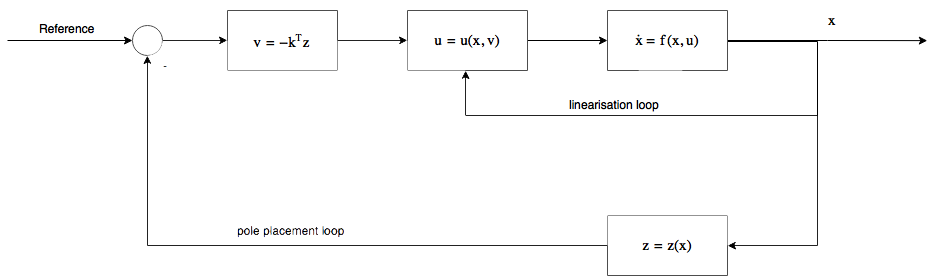
\includegraphics[width=1\textwidth]{Figures/NLI}
  \caption[Feedback linearisation example]{Feedback linearisation example \cite{Slotine+Li}}
  \label{fig:nli}
\end{figure}

To better understand Input-Output linearisation, some mathematical tools must firstly be described. One of these tools is the Lie derivative, that represents the gradient of a given scalar function $h(x)$ projected along a given vector function $f(x)$. Such a Lie derivative is therefore represented as

\begin{equation}
L_fh(x) = \nabla h(x)f(x) = \Sigma^n_{i=1}\dfrac{\partial h(x)}{\partial x_i}f_i(x)
\end{equation}

A Lie derivative can also be applied multiple times, resulting in a $k^{th}$ order Lie derivative

\begin{equation}
L^k_fh(x)=L_f\left(L^{k-1}_fh(x)\right)=\nabla \left(L^{k-1}_fh(x)\right)f(x) \quad \text{with} \quad L^0_fh(x)=h(x)
\end{equation}

The second operator from Lie algebra to be introduced here, quite important in Input-Output linearisation is the Lie bracket, and these are defined as, given two vector fields $f$ and $g$,

\begin{equation}
[f,g] = ad_f g = \nabla g f - \nabla f g
\end{equation}

Once again Lie brackets can be defined recursively as

\begin{equation}
ad_f^ig=[f, ad_f^{i-1}g] \quad \text{with} \quad ad_f^0g=g
\end{equation}

Finally, the concept of \emph{diffeomorphism} must be described to fully understand this control technique. According to \cite{Slotine+Li}, it is a generalisation of the concept of coordinate transformation, and is formally stated as:

\emph{A function $\phi: R^n\rightarrow R^n$, defined in a region $\Omega$, is called a diffeomorphism if it is smooth and its inverse $\phi^{-1}$ exists and is smooth \cite{Slotine+Li}}. 
In Input-Output linearisation, a \emph{diffeomorphism} must be found to transform a non-linear system into a linear one.
\subsection{SISO systems}
\label{section:background/SISO_NLI}

Although an aircraft is always considered as a MIMO system, a description of this control concept will firstly be provided for a general SISO case, before generalising to a MIMO case. Nonlinear systems that can be represented as affine systems $\dot{x}=f(x)+g(x)u$ will be discussed in this section. From \cite{Slotine+Li}, a definition of Input-State linearisation is to find, for a nonlinear system of relative degree $n$, a \emph{diffeomorphism} $\phi:\Omega \rightarrow R^n$ and nonlinear control law
\begin{equation}
u=\alpha(x) + \beta(x)\upsilon
\label{eq:nli_control_law}
\end{equation}

such that the new state variables $z=\phi(x)$ and \emph{pseudo-input} $\upsilon$ satisfy the linear time invariant system $\dot{z} = Az+B\upsilon$, where the following equations are satisfied

\begin{equation}
	\begin{cases}
		\dot{z_i}=z_{i+1} & if\quad i<n\\
		\dot{z_n}=\upsilon & if\quad i=n
	\end{cases}
	\label{eq:SISO_state}
\end{equation}

In order to find such a function and control law, one must find a state $z_1$ such that 
\begin{subequations}
	\begin{equation}
		\nabla z_1 ad_f^ig=0 \qquad i=0, ..., n-2
	\end{equation}
	\begin{equation}
		\nabla z_1 ad_f^{n-1}g\neq 0
	\end{equation}
\end{subequations}

The remaining states are then obtained from $z(x) = [z_1 \quad L_fz_1 \quad ... \quad L_f^{n-1}z_1]^T$ and the input transformation from

\begin{subequations}
	\begin{equation}
		\alpha (x) = - \dfrac{L_f^nz_1}{L_gL_f^{n-1}z_1}
	\end{equation}
	\begin{equation}
		\beta (x) = \dfrac{1}{L_gL_f^{n-1}z_1}
	\end{equation}
\end{subequations}

\subsection{MIMO systems}
\label{section:background/MIMO_NLI}

These concepts can also be extended to MIMO systems in a similar manner, by differentiating the outputs until the inputs explicitly appear. This time however, there are individual relative degrees per output. The sum of these relative degrees is called total degree $r$ and must satisfy $r\leq n$, $n$ being the order of the system. Note however, that in the case of $r<n$, a part of the system dynamics is rendered unobservable in the input-output linearisation, as the closed loop dynamics will have a lower order $r$ than the whole dynamics of the system $n$. These internal dynamics must therefore be studied to establish the effectiveness of the feedback linearisation. For the case where the internal dynamics is stable, the input-output linearisation method can then be used. In the case of unstable internal dynamics however, these would lead to both undesirable and uncontrollable phenomena, in which case a different control design is needed.

Given a MIMO system 
\begin{gather}
\dot{x} = f(x) + G(x)u\\
y=h(x)
\end{gather}
the $\phi$ functions are defined as $\phi^i_j(x)=L^{j-1}_fh_i(
x)$ and satisfy a condition similar to \ref{eq:SISO_state} 
\begin{equation}
\dot{\phi}^i_1(x)=\phi^i_2,...,\dot{\phi}^i_{r_i-1}=\phi^i_{r_i} \quad \text{and} \quad \dot{\phi}^i_{r_i}=L_f^{r_i}h_i(x)+\sum^m_{j=1}L_{g_j}L^{r_i-1}_fh_i(x)u_j
\end{equation}
As this equation holds for $1<i<p$, $p$ being the number of outputs of the system, giving an expression for the pseudo control input $\upsilon$
\begin{equation}
\upsilon = 
\begin{bmatrix}
\dot{\phi}^1_{r_1}\\
\vdots\\
\dot{\phi}^p_{r_p}\\
\end{bmatrix}
\end{equation}

It is also interesting to note the resulting system is not only linear, but also completely decoupled, as each new pseudo input only affects one output.

\section{Limitations of feedback linearisation}
\label{section:background/limitations}
Although feedback control answers to many of the problems of linear controllers such as PID and LQR, it has a some downsides. Indeed, being a model based controller, it requires the system model to be quite accurately known, and parameter uncertainties can lead to undesired responses. Let $\upsilon$ be the vector of pseudo inputs, for a second order $\ddot{x} = f(x,\dot{x},u)$, if it is input-output linearisable and the exact system is known, then it comes that, from \cite{YANG+LIN_Adaptive_Flight_Control}
\begin{equation}
\ddot{x}=\upsilon
\end{equation}
However, even for simpler models, a real system is difficult to accurately describe, and an approximation $\hat{f}$ of $f$ is usually chosen, resulting in $\upsilon=\hat{f}(x,\dot{x},u)$. Therefore, defining a dynamic inversion error, $\Delta(x,\dot{x},u)=f(x,\dot{x},u)-\hat{f}(x,\dot{x},u)$, comes that, as stated in \cite{YANG+LIN_Adaptive_Flight_Control}
\begin{equation}
\ddot{x}=\upsilon + \Delta(x,\dot{x},u)
\label{eq:system+error}
\end{equation}
There can be many causes for a dynamic inversion error to be present, as not only modelling incertitudes can lead to larger errors, but also external interference (wind gusts) and actuator faults. The goal of this section will be to present the reader with some solutions to minimize this error. 

\subsection{Fuzzy Logic Systems}
\label{section:background/fuzzy_logic}

Fuzzy logic systems are based on the paradigm of continuous levels of truth between 0 and 1, rather than the usual discrete true or false levels of truth. Using these continuous truth values, a set of IF-ELSE rules is chosen. The goal of this type of controller is to duplicate the way a pilot would respond to a given flight situation. These rules can base their control input on variables such as roll, angle of attack and sideslip \cite{Comparison_IntelligentSys}. This control method is based on three main parts. The first one if \textit{fuzzification}, that consists of converting the plant outputs to fuzzy logic values. \textit{Rule-based inference}, using the previously mentioned set of rules, a fuzzyfied control input is computed, which then goes through the \textit{defuzzyfication} part of the control algorithm. 
Fuzzy systems have some advantages: its linguistic interpretation of human knowledge facilitate the interpretation of results, and the knowledge base can be improved through addition of new rules. However, this method comes with some disadvantages. First of all, the set of rules that will improve the control of the aircraft is entirely dependent on expert knowledge, thus resulting in an empiric set of rules. This also means the method has no capability of generalization, as the control is only applied to specific cases, of the form "if the error is greater than a given value, apply this compensation to control input". It is also not robust to topological changes of the system \cite{Neuro_fuzzy_survey}. For these reasons this method will not be further studied and implemented in this work.


\subsection{Neural Networks}
\label{section:background/NN}

Artificial Neural Networks (NN) are a biologically inspired simulation of the brain nervous system. They are composed of simulated neurons and synapses. The sum of the inputs of a neuron are summed and the result is fed into an activation function, which then return a bounded value, either between -1 and 1 or 0 and 1. The inputs and outputs of a neuron are multiplied by a weight, representing the synapses between neurons. We get the following equation for one neuron
\begin{equation}
y(x_1,x_2,...,x_n)=f((\sum ^n_{i=1} w_i x_i)+b)
\end{equation}
where $b$ is a bias term and $f$ a given activation function. Neurons are then set in three different types of layers: the input, the output and the hidden layers. These are connected between each other, and the hidden part can be composed of several layers. The weights can then be tuned based on experience, making it suitable for intelligent learning. To tune these weights learning algorithms are used. There are two types of learning algorithms: batch and online training. It is called training to the process of iteratively reaching the ideal set of weights that will minimise the error between the output of the neural network and that of a given unknown function.

Batch training is mostly based on a property of Neural Networks that, according to the Universal Approximation Theorem showed in 1989 by George Cybenko, a feed forward neural network can approximate any continuous function. The network is trained by providing input and output pairs. The weights are found in order to approximate the output of the neural network to that of the original function. Once these weights are computed, the network can then be used to compute outputs from inputs that were not part of the initial knowledge of input-output pairs.

Although this learning method approach is used in many of NN applications, it cannot however be easily used to improve an existing feedback linearisation  controller, as it requires an \textit{a priori} knowledge of the modelling error for each given input.

Online training, contrary to batch training, can deal with dynamically changing environments. This training paradigm is not based on an \textit{a priori} knowledge set, and instead relies on update laws that compute the new weights after each control iteration. It is this method that will be retained to adaptively correct the inversion error from the feedback linearisation. Training a network online, however, is less trivial when compared to batch training. An algorithm named backpropagation will be presented to provide a way of training a network online. A description on the implementation of the neural network and how it will be used to improve the feedback linearisation controller will be given on chapter \ref{chapter:implementation}.


%Backprop
The backpropagation algorithm is one of the most common NN training algorithm, commonly used in batch training, to update the weights of each layer of a network, in order to minimize a cost function. However, research has been done in order to use backpropagation techniques to create online adaptive and augmented control such as \cite{online_adaptiveNN}, \cite{UAV_adaptive}, \cite{UAV_adaptive2}. Indeed, it is also possible to use such algorithms to continuously update the weights of a network as the data is generated. Backpropagation can only be implemented if the activation function of the NN is differentiable. 

The backpropagation algorithm can be described by a two phase cycle, Propagation and Weight update. During this last phase the gradient descent algorithm is used to optimize a cost function. As such, a cost function $E$ must be chosen, and must be a function of the outputs of the neural network. A commonly used error function is 
\begin{equation}
E=\frac{1}{2} (y_d-y)^2
\end{equation}

Where $y_d$ is the desired output of the network and $y$ is the actual output of the network. The $\frac{1}{2}$ factor is added to be cancelled when differentiating. For a given neuron $i$, the sum of its inputs $sum_i$ is given by
\begin{equation}\label{eq:def_sum}
sum_i = \sum ^n_{k=1} w_{ki} x_k
\end{equation}
Where $w_{ki}$ is the weight of the $k^{th}$ input of neuron $i$, and $x_k$ are the outputs of the neurons form the previous layer. Given an activation function $f(x)$, we define the output of neuron $i$ as 
\begin{equation}\label{eq:NN_output}
x_i = f(sum_i)
\end{equation}

In order to use the gradient descent algorithm, the derivative of the cost function with respect to a given weight $w_{ij}$ must be computed. To do so, the chain rule is used as
\begin{equation}\label{eq:gradient}
\frac{\partial E}{\partial w_{ij}} = \frac{\partial E}{\partial x_j}\frac{\partial x_j}{\partial sum_j}\frac{\partial sum_j}{\partial w_{ij}}
\end{equation}
These three factors can now be easily computed. The last two factors are independent of weather $x_j$ is a hidden or output layer and will for this reason be calculated firstly. From \ref{eq:def_sum} and \ref{eq:NN_output} comes that
\begin{equation}
\frac{\partial x_j}{\partial sum_j} = \frac{\partial f(sum_j)}{\partial sum_j}
\end{equation}
For an output layer, where values may be unbounded, linear output functions may be used, for which the equation above has a trivial solution. For output layers of classification neural networks or for hidden layers in general, logistic or tangent sigmoid functions can be used instead. For the first case let $f(x)=\frac{1}{1+e^{-x}}$, then

\begin{equation}
\frac{\partial f(sum_j)}{\partial sum_j}=f(sum_j)(1-f(sum_j))
\end{equation}
For the case of a tangent sigmoid activation function $f(x)=tanh(x)$ comes
\begin{equation}
\frac{\partial f(sum_j)}{\partial sum_j}=1-f^2(sum_j)
\end{equation}
For the term $\frac{\partial sum_j}{\partial w_{ij}}$, from \ref{eq:def_sum} this partial derivative is easily computed

\begin{equation}
\frac{\partial sum_j}{\partial w_{ij}} = \frac{\partial \left(\sum ^n_{k=1} w_{kj} x_k\right)}{\partial w_{ij}} = x_i
\end{equation}
For the output layer, the first term of equation \ref{eq:gradient} can easily be evaluated, as $x_j=y$ for such a case, giving
\begin{equation}
\frac{\partial E}{\partial x_j}=\frac{\partial (\frac{1}{2} (y_d-y)^2)}{\partial y}= y-y_d
\end{equation}
For input layers however, this derivative is less obvious to estimate. One can consider that the error function $E$ is a function of the inputs of all neurons that take $x_j$ as input. Let $S$ be such a set of inputs, from the total derivative to $x_j$ comes that
\begin{equation}
\frac{\partial E}{\partial x_j} = \sum _{s\in S}\left( \frac{\partial E}{\partial x_s}\frac{\partial x_s}{\partial sum_s}\frac{\partial sum_s}{\partial x_j}\right)=\sum _{s\in S}\left( \frac{\partial E}{\partial x_s}\frac{\partial f(sum_s)}{\partial sum_s}w_{js}\right)
\end{equation}
Note that the term $ \frac{\partial E}{\partial x_s} $ represent the all the derivatives of the errors with respect to the outputs of the next layer of neurons. Taking into account that the last layer is easily evaluated without this method, the derivatives of all hidden neurons can be computed. Knowing the value of \ref{eq:gradient}, an update law for the weights can now be stated from the gradient descent algorithm
\begin{equation}\label{eq:update_law}
\Delta w_{ij} = - \alpha \frac{\partial E}{\partial w_{ij}}
\end{equation}
Where $\alpha$ is a learning coefficient, and its choice is crucial to assure a fast convergence of the solution. Indeed, while a exceedingly large learning coefficient can cause this algorithm to miss the minimum error, a small learning coefficient will also increase the convergence rate. The $-1$ factor is added in the equation above to converge to a local minima, removing it would make this algorithm maximize the cost function. A limitation of the backstepping algorithm that must also be taken into account is that it only guarantees local minima convergence. 
A detailed description on the connection of this algorithm with the control of the aircraft will be given on the next chapter.
 % file "Thesis_Background.tex"
\cleardoublepage

%%%%%%%%%%%%%%%%%%%%%%%%%%%%%%%%%%%%%%%%%%%%%%%%%%%%%%%%%%%%%%%%%%%%%%%%
%                                                                      %
%     File: Thesis_Implementation.tex                                  %
%     Tex Master: Thesis.tex                                           %
%                                                                      %
%     Author: Andre C. Marta                                           %
%     Last modified :  2 Jul 2015                                      %
%                                                                      %
%%%%%%%%%%%%%%%%%%%%%%%%%%%%%%%%%%%%%%%%%%%%%%%%%%%%%%%%%%%%%%%%%%%%%%%%

\chapter{Implementation}
\label{chapter:implementation}

This section will go in depth into the implementation of the concepts presented in chapter \ref{chapter:background}. The plane model to be controlled is first implemented and verified. The first goal after this first step is to design a controller that will allow the aircraft to follow a trajectory from several position waypoints through time. The influence of certain parameters and knowledge of the exact plane model will be studied and discussed in chapter \ref{chapter:results}. The final goal will be to improve the controller and its robustness by reducing tracking error through the use of an adaptive neural network.

%%%%%%%%%%%%%%%%%%%%%%%%%%%%%%%%%%%%%%%%%%%%%%%%%%%%%%%%%%%%%%%%%%%%%%%%
\section{Plane Model}
\label{section:model}
The work made in this thesis was built on top of the work done by H. Escamilla Nuñez and  F. Mora Camino on 4D trajectory tracking \cite{hector}. The model used in this work is a six degree of freedom transport aircraft that will be described in this section. 

\subsection{Frames of Reference}
\label{section:background/model/for}
The first step before describing the dynamics of a commercial aircraft will be to define the frames of reference used to do so. The first frame of reference, on which 4D trajectories are described, corresponds to the WGS84 frame of reference. A second frame of reference corresponding to the aircraft body frame will be used to provide its fast rotational dynamics. Lastly all aerodynamic forces will be applied in the axial directions of the wind frame. This frame is aligned with the wind speed vector relative to the airplane, given by both the angle of attack $\alpha$ and the sideslip angle $\beta$. For these last two frames of reference, a rotation matrix can be defined from wind frame to body frame by


\begin{equation}
R_{BW}=
\begin{bmatrix}
c_\alpha c_\beta & -c_\alpha s_\beta & -s_\alpha \\
s_\beta & c_\beta & 0 \\
s_\alpha c_\beta & -s_\alpha s_\beta & c_\alpha
\end{bmatrix}
\label{eq:wind2body}
\end{equation}

To describe the attitude of the plane Euler, roll, pitch and yaw angles, will also be used, namely $\phi\{-\pi,\pi\}; \theta \{-\dfrac{\pi}{2},\dfrac{\pi}{2}\}; \psi \{-\pi,\pi\}$. From these angles the rotation matrix from the body to the earth frame is given by

\begin{equation}
R_{EB}=
\begin{bmatrix}
c_\theta c_\psi & s_\phi s_\theta c_\psi - c_\phi s_\psi & c_\phi s_\theta c_\psi + s_\phi s_\psi \\
c_\theta c_\psi & s_\phi s_\theta s_\psi + c_\phi c_\psi & c_\phi s_\theta s_\psi - s_\phi c_\psi \\
-s_\theta & s_\phi c_\theta & c_\phi c_\theta
\end{bmatrix}
\label{eq:body2earth}
\end{equation}

\subsection{Fast Dynamics}
\label{section:background/model/fast_dynamics}

The considered actuators of the aircraft that control its attitude are given by the control surface deflection $\delta = [\delta_{ail} \delta_{ele} \delta_{rud}]^T$, each applying a torque along an axis of the body frame. These torques are given by

\begin{equation}
\begin{bmatrix}
L'\\
M\\
N
\end{bmatrix}
= \dfrac{1}{2}\rho S V_a^2\left(
\begin{bmatrix}
bC_l\\
\bar{c}C_m\\
bC_n
\end{bmatrix}
+ C_\delta \delta\right)
\label{eq:torque}
\end{equation}

where $\bar{c}$ and $b$ represent the wing mean chord and its span respectively, $C_\delta$ and the moment coefficients $[C_l C_m C_n]^T$ are given by

\begin{equation}
C_\delta = 
\begin{bmatrix}
bC_{l\delta_{ail}} & 0 & bC_{l\delta_{rud}} \\
0 & \bar{c}C_{m\delta_{ele}} & 0 \\
bC_{n\delta_{ail}} & 0 & bC_{n\delta_{rud}}\\
\end{bmatrix}
\label{eq:cdelta}
\end{equation}
\begin{equation}
\begin{bmatrix}
C_l\\
C_m\\
C_n
\end{bmatrix} 
=
\begin{bmatrix}
C_{l\beta} \beta + C_{l_p} p \dfrac{b}{2V_a} + C_{l_r} r \dfrac{b}{2V_a}\\
C_{m_0} + C_{m_\alpha} \alpha + C_{m_q} q \dfrac{\bar{c}}{2V_a}\\
C_{n\beta} \beta + C_{n_p} p \dfrac{b}{2V_a} + C_{n_r} r \dfrac{b}{2V_a}
\end{bmatrix}
\label{eq:cmoment}
\end{equation}
Where $p, q, r$ are the body angular rates ($\Omega = [p\quad q\quad  r]^T$) and $V_a$ is the airspeed. The method for obtaining the coefficients of equation \ref{eq:cmoment} will be provided in the chapter to follow. Having defined the torques applied to the aircraft the rotational dynamics equation can now be stated as per \cite{hector}, $I$ being the aircraft inertial matrix.
\begin{subequations}
	\begin{equation}
		\dot{\Omega} = I^{-1} M_{ext} - I^{-1}\Omega \times (I\Omega)
	\end{equation}
	\begin{equation}
		\dot{\Omega} = 
		\dfrac{1}{2}\rho S I^{-1} V_a^2\left(
		\begin{bmatrix}
			bC_l\\
			\bar{c}C_m\\
			bC_n
		\end{bmatrix}
		+ C_\delta \delta\right)
		- I^{-1}\Omega \times (I\Omega)	
	\end{equation}

\label{eq:fast_dynamics}
\end{subequations}

These two equations can be rearranged to account for the effect of the wind, allowing further on to simulate the behaviour of the airplane in the presence of wind disturbances. Let $\vec{V_G} = [u \quad v \quad w]^T$ be the speed of the CG relative to the ground, $\vec{V}$ the speed of the CG relative to the air mass and $\vec{W}$ the speed of the wind relative to the ground, then as per Etkin and Reid \cite{Etkin+Reid} 
\begin{equation}
\vec{V_G} = \vec{V} + \vec{W} = 
\begin{bmatrix}
V_ac_\alpha c_\beta + V_{w_x}\\
V_as_\beta+V_{w_y}\\
V_as_\alpha c_\beta + V_{w_z}
\end{bmatrix}
\label{eq:windtriangle}
\end{equation}
and $\alpha$ and $\beta$ can be computed by 
\begin{subequations}
	\begin{equation}
		\alpha = arctan\left(\dfrac{w-V_{w_z}}{uV_{w_x}}\right)
		\label{eq:alpha}
	\end{equation}
	\begin{equation}
		\beta = arctan\left(\dfrac{v-V_{w_y}}{V_a}\right)
		\label{eq:beta}
	\end{equation}
\end{subequations}

From these three equations, differentiating \ref{eq:alpha} and \ref{eq:beta}, and from equation \ref{eq:windtriangle} and the translation dynamics equation \ref{eq:boddy_acc} comes that 

\begin{equation}
\begin{bmatrix}
\dot{\alpha}\\
\dot{\beta}\\
\dot{V_a}
\end{bmatrix}
= 
\begin{bmatrix}
H_{11} & H_{12} & H_{13}\\
H_{21} & 0 & H_{23}\\
H_{31} & H_{32} & H_{33}
\end{bmatrix}
\begin{bmatrix}
p\\
q\\
r
\end{bmatrix}
+
\begin{bmatrix}
Q_1\\
Q_2\\
Q_3
\end{bmatrix}
\label{eq:alphabetadot}
\end{equation}
Where the entries of the matrix are given by

\begin{gather*}
H_{11}=\dfrac{-V_a c_\alpha s_\beta  c_\beta - V_{w_y} c_\alpha c_\beta}{V_a(1+\tan^2\alpha)c^2_\alpha c^2_\beta}\\
H_{12}=\dfrac{V_a(c^2_\alpha c^2_\beta-s^2_\alpha c^2_\beta) + V_{w_x}c_\alpha c_\beta - V_{w_z}s_\alpha s_\beta}{V_a(1+\tan^2\alpha)c^2_\alpha c^2_\beta}\\
H_{13}=\dfrac{-V_a s_\alpha s_\beta  c_\beta - V_{w_y} s_\alpha c_\beta}{V_a(1+\tan^2\alpha)c^2_\alpha c^2_\beta}\\
H_{21}=\dfrac{V_a s_\alpha c_\beta + V_{w_z}}{V_a c_\beta}\\
H_{23}=-\dfrac{V_a c_\alpha c_\beta + V_{w_x}}{V_a c_\beta}\\
H_{31}=2 \left(-V_a s_\beta s_\alpha c_\beta - V_{w_x} s_\alpha c_\beta \right)\\
H_{32}=2\left( -V_{w_z} c_\alpha c_\beta + V_as_\alpha c_\beta s_\beta
 + V_{w_z}s_\beta + V_{w_x}s_\alpha c_\beta \right)\\
H_{33}=2\left(V_{w_y}c_\alpha c_\beta - V_{w_x}s_\beta\right)\\
Q_1=\dfrac{\left(\dfrac{1}{m}F_{za} + gc_\theta c_\phi - \dot{V}_{w_z} \right)c_\alpha c_\beta - \left(\dfrac{1}{m}(F_{xa} + T)-gs_\theta - \dot{V}_{w_x}\right)}{V_a(1+\tan^2\alpha)c^2_\alpha c^2_\beta}\\
Q_2=\dfrac{\dfrac{1}{m}F_{ya}+g c_\theta s_\phi-\dot{V}_{w_y}}{c_\beta}\\
Q_3=2 \left( \left(\dfrac{-1}{m}(F_{xa}+T) + g s_\theta - \dot{V}_{w_x} \right)c_\alpha c_\beta + \left( \dfrac{-1}{m}F_{ya} - \dot{V}_{w_y} \right)s_\beta + \left(\dfrac{-1}{m}F_{za} - \dot{V}_{w_z} \right)s_\alpha c_\beta \right)
\label{eq:Ra_dot}
\end{gather*}
The forces in the air frame $F_{xa}, F_{ya}, F_{za}$ will be further detailed in the next section on translation dynamics. 

The angular rates are also related to the Euler angles. The relationship between the Euler angles and the rotation rates is also one that will prove useful when implementing the model in a Matlab simulation, and is given by

\begin{equation}
\begin{bmatrix}
\dot{\phi}\\
\dot{\theta}\\
\dot{\psi}
\end{bmatrix}
=
\begin{bmatrix}
1 & tg_\theta s_\phi & tg_\theta c_\phi\\
0 & c_\phi & -s_\phi\\
0 & \dfrac{s_\phi}{c_\theta} & \dfrac{c_\phi}{c_\theta}
\end{bmatrix}
\begin{bmatrix}
p\\
q\\
r
\end{bmatrix}
\label{eq:euler2omega}
\end{equation}

\subsection{Translation Dynamics}
\label{section:background/model/guidance_dynamics}

This subsection focuses on the forces applied to aircraft, introducing a new actuation variable, the thrust force $T$. These forces are applied along the three axes of the wind frame, lift, drag and side force, given by
\begin{equation}
\begin{bmatrix}
D\\
Y\\
L
\end{bmatrix}
= \dfrac{1}{2} \rho SV_a^2
\begin{bmatrix}
C_D\\
C_Y\\
C_L
\end{bmatrix}
\label{eq:forces}
\end{equation}
Once again, the method used to compute these coefficients will be given in the chapter \ref{chapter:implementation} in detail. These coefficients, similarly to the moment coefficients, are functions of the angle of attack, sideslip angle and airspeed, the three most relevant variables when determining aerodynamic forces and moments. Although aerodynamic forces are usually expressed in the wind frame, as the thrust is always applied along the $x$ axis of the body frame, it is necessary to rotate the aerodynamic forces to this frame. This way the sum of the airplane forces can be obtained. 

\begin{equation}
\begin{bmatrix}
F_{xa}\\
F_{ya}\\
F_{za}
\end{bmatrix}
= R_{WB}
\begin{bmatrix}
-D\\
Y\\
-L
\end{bmatrix}
\label{eq:body_forces}
\end{equation}
From Newton's Second Law comes the aircraft acceleration

\begin{equation}
\begin{bmatrix}
\dot{u}\\
\dot{v}\\
\dot{w}
\end{bmatrix}
=
\begin{bmatrix}
\dfrac{1}{m}(F_{xa} + T) - gs_\theta +rv-qw\\
\dfrac{1}{m}F_{ya} + gc_\theta s_\phi + pw - ru\\
\dfrac{1}{m}F_{za} + gc_\theta c_\phi + qu - pv
\end{bmatrix}
\label{eq:boddy_acc}
\end{equation}

An expression in the Earth frame can also be obtained

\begin{equation}
\begin{bmatrix}
\ddot{x}_E\\
\ddot{y}_E\\
\ddot{z}_E
\end{bmatrix}
= \dfrac{1}{m} R_{BE}
\begin{bmatrix}
F_{xa}+T\\
F_{ya}\\
F_{za}
\end{bmatrix}
+
\begin{bmatrix}
0\\
0\\
g
\end{bmatrix}
\end{equation}

\subsection{Actuator Dynamics}
\label{section:background/model/actuator_dynamics}

Finally, to simulate the delay response in actuation in order to have a realistic simulation, first order systems were introduced to the actuator dynamics as per \cite{hector}. For the control surfaces $\delta_i$, given a desired $\delta_i^d$ comes

\begin{equation}
\dot{\delta_i} = \dfrac{1}{\xi_i}(\delta_i^d-\delta_i)
\label{eq:actuator_dynamics}
\end{equation}

Similarly for thrust

\begin{equation}
\dot{T} = \dfrac{1}{\xi_T}(T^d-T)
\end{equation}

$\xi_i$ and $\xi_T$ are time constants. As the responsiveness of the resultant thrust will be much slower than that of the control surfaces, $\xi_T>>\xi_i$.
The chosen commercial aircraft that will be simulated is the Boeing 737-200, an aircraft with over 30 years of service for which some information of flight parameters is readily available, such as weight, wing span and mean chord. The simulation was made in a cruise flight environment, at $200$ m/s velocity at $10000$ m above the ground. The chosen inertial matrix for this aircraft is given by
\begin{equation}
\begin{bmatrix}
1278369.56 & 0 & -135588.17\\
0 & 3781267.79 & 0\\
-135588.17 & 0 & 4877649.98
\end{bmatrix}
kg.m^2
\end{equation}
The ISA atmospheric model was used to compute the air density at any given height.
\begin{table}[H]
  \centering
  \caption{Boeing 737-2 parameters}
    \begin{tabular}{rr}
    \toprule
    Weight $m$ & $52390$ kg \\
    Wing Span $b$ & $28.35$ m \\
    Wing Area $S$ & $102.0$ m$^{2}$ \\
    Wing mean chord $\bar{c}$ & $4.35$ m \\
    Length $l$ & $30.53$ m \\
    \bottomrule
    \end{tabular}%
  \label{tab:b737_parameters}
\end{table}%

The time constants used for the actuators was $\xi_{\delta_i}50$ms and $\xi_T=4$s for the engines.
\subsection{Airplane Parameters and Coefficients}
\label{section:model/plane_dynamics}

In order to simulate the aircraft fast dynamics, its moments must first be computed to use equation \ref{eq:fast_dynamics}. The torque caused by the actuators is modelled as equation \ref{eq:cdelta}, using
\begin{gather*}
C_{L_{\delta_{ail}}}=0.02 \quad rad^{-1}\\
C_{L_{\delta_{rud}}}=0.002 \quad rad^{-1}\\
C_{M_{\delta_{ele}}}=-0.003 \quad rad^{-1}\\
C_{N_{\delta_{ail}}}= -0.002 \quad rad^{-1}\\
C_{N_{\delta_{rud}}}= -0.07 \quad rad^{-1}
\end{gather*}
The remaining aerodynamic coefficients from equation \ref{eq:cmoment} were obtained from the work of Hector Escamilla Nuñez in \cite{hector}.

In this work, neural networks were used to interpolate data from the USAF Stability and Control Digital Data Compendium. A two layer feed forward network, with a hidden sigmoid activation function and a linear output activation function, was then trained using the gathered data with the Bayesian Regulation training algorithm \cite{hector}. Indeed as stated previously, neural networks can approximate any continuous function according to the Universal Approximation Theorem. This method is therefore optimal to accurately approximate the variation of these coefficients that mainly vary with the angle of attack $\alpha$ and airspeed $V_a$. The only exception to this method was the drag coefficient, given for this aircraft by
\begin{equation}
C_D=0.0176+0.0515 C_L^2
\label{eq:cd_cl}
\end{equation}

The sum of the moments can be computed and used to obtain the rotation rates $p$, $q$ and $r$. Equation \ref{eq:euler2omega} can also be used and integrated to obtain the Euler angles. These will also be necessary for frame of reference changes, namely from body to earth and vice-versa. The aerodynamic forces were computed from equation \ref{eq:forces} using the outputs of the neural networks. The body forces and acceleration relative to the earth frame were then obtain from equations \ref{eq:body_forces} and \ref{eq:boddy_acc}. 
The effects of the wind were also taken into account by adding the wind speed to the integration of the acceleration of the aircraft relative to the earth as per \ref{eq:windtriangle}. At this point the values of $\alpha$ and $\beta$ were also obtained for their respective equations \ref{eq:alpha} and \ref{eq:beta}. 

A simplified block diagram of the plane simulator is given by figure \ref{fig:plane_model}.
\begin{figure}[!htb]
  \centering
  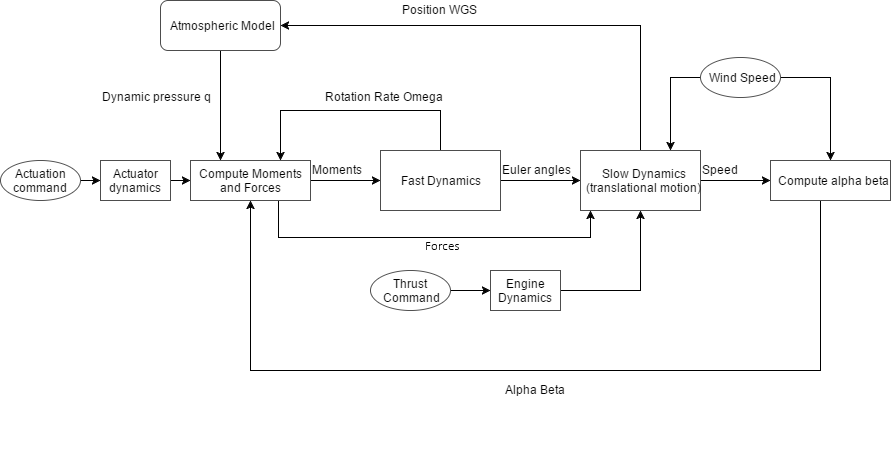
\includegraphics[width=1\textwidth]{Figures/PlaneModel.png}
  \caption[Plane dynamics simulator diagram]{Plane dynamics simulator diagram}
  \label{fig:plane_model}
\end{figure}
 

\section{Controller Implementation}
\label{section:control_implement}

To invert such a complex system (figure \ref{fig:plane_model}), two layers of inversion are proposed by H. Escamilla \cite{hector}, namely for the fast and slow dynamics. Directly controlling these are three of the four actuator control inputs, the control surfaces for the aileron, elevon and rudder. These will therefore be the output of the nonlinear inversion control. 

\subsection{Fast Dynamics}
To invert the fast dynamics equation \ref{eq:fast_dynamics} must be differentiated once, to account for both the actuator dynamics \ref{eq:actuator_dynamics} and the wind effects. Doing so yields the jerk vector given by, as per \cite{hector}

\begin{equation}
\begin{bmatrix}
\ddot{p}\\
\ddot{q}\\
\ddot{r}
\end{bmatrix}
= \dfrac{1}{2}\rho SI^{-1} \left\lbrace V_a^2 C_\delta \xi^{-1}
\begin{bmatrix}
\delta^d_{ail}-\delta_{ail}\\
\delta^d_{ele}-\delta_{ele}\\
\delta^d_{rud}-\delta_{rud}
\end{bmatrix}
+V_a^2C_c\dot{R_a}+2V_a\dot{V_a}\left(
\begin{bmatrix}
bC_l\\
\bar{c}C_m\\
bC_n
\end{bmatrix}
+ C_\delta 
\begin{bmatrix}
\delta_{ail}\\
\delta_{ele}\\
\delta_{rud}
\end{bmatrix}
\right) \right \rbrace + I^{-1}\left(\dfrac{1}{4}\rho SV_aC_k-I_n\right)\dot{\Omega}
\label{eq:jerk}
\end{equation}

where

\begin{gather*}
I=
\begin{bmatrix}
A & 0 & -E\\
0 & B & 0\\
-E & 0 & C
\end{bmatrix}\\
I_n=
\begin{bmatrix}
-Eq & (C-B)r-Ep & (C-B)q\\
(A-C)r+2Ep & 0 & (A-C)p-2Er\\
(B-A)q & (B-A)p+Er & Eq
\end{bmatrix}\\
\xi=
\begin{bmatrix}
\xi_{ail} & 0 & 0\\
0 & \xi_{ele} & 0\\
0 & 0 & \xi_{rud}
\end{bmatrix}\\
C_c=
\begin{bmatrix}
0 & bC_{l_\beta} & -\dfrac{b^2}{2V_a^2}(C_{l_p}p+C_{l_r}r)\\
\bar{c}C_{m_\alpha} & 0 & -\dfrac{\bar{c}^2}{2V_a^2}C_{m_q}q\\
0 & bC_{n_\beta} & -\dfrac{b^2}{2V_a^2}(C_{n_p}p+C_{n_r}r)
\end{bmatrix}\\
C_k=
\begin{bmatrix}
b^2C_{l_p} & 0 & b^2C_{l_r}\\
0 & \bar{c}^2C_{m_q} & 0\\
b^2C_{n_p} & 0 & b^2C_{n_r}
\end{bmatrix}\\
\dot{Ra} =  [\dot{\alpha} \quad \dot{\beta} \quad \dot{V_a}]^T
\end{gather*}

To do a feedback linearisation, a pseudo input must be chosen, in this case $\tau = \ddot{\Omega}$. The feedback control law will therefore be, solving equation \ref{eq:jerk} for $\delta^d$,

\begin{equation}
\begin{bmatrix}
\delta^d_{ail}\\
\delta^d_{ele}\\
\delta^d_{rud}
\end{bmatrix}
=\dfrac{1}{V_a^2}\xi C_\delta^{-1}\left\lbrace\dfrac{2I}{\rho S}\tau - \dfrac{2}{\rho S}(\dfrac{1}{4}\rho S V_aC_k - I_n)\dot{\Omega} -2V_a\dot{V_a} \left(
\begin{bmatrix}
bC_l\\
\bar{c}C_m\\
bC_n
\end{bmatrix}
+ C_\delta \delta\right)-V_a^2C_c\dot{R_a} \right\rbrace+ \delta
\label{eq:control_law}
\end{equation}


Indeed, by replacing \ref{eq:control_law} in the jerk equation \ref{eq:jerk}, the equation $\ddot{\Omega} = \tau$ is obtained, resulting in a successfully inverted system.


The wind effects will appear in the terms including $\dot{R}_a =  [\dot{\alpha} \quad \dot{\beta} \quad \dot{V_a}]^T$, as the equation defining $\dot{V_a}$ can be obtained differentiating the norm of the speed relative to the ground. The value of $\dot{R}_a$ can be computed from equation \ref{eq:Ra_dot}.

Should all of the parameters mentioned in the equations above be known and no inversion error be made, the resulting system $\ddot{\Omega}=\tau$ will be both linear and decoupled, having three pseudo inputs $\tau = [\tau_p \quad \tau_q \quad \tau_r]^T$. As mentioned in section \ref{section:background/NLI}, the next step of the nonlinear inversion shall be to propose a linear controller for this resulting system. Taking the desired rotation rates $\Omega^d$ as inputs comes a control law for $\tau$, first considering without neural network adaptation
\begin{equation}
\tau = -K_P (\Omega-\Omega^d)-K_D (\dot{\Omega}-\dot{\Omega}^d)+\ddot{\Omega}^d
\label{eq:linear_controller}
\end{equation}
Where $K_P$ and $K_D$ are chosen to ensure stability and reference tracking. The previous equation can also be written as
\begin{equation}
\ddot{e}=-K_P e - K_D \dot{e}
\end{equation}
assuming that an ideal inversion is obtained and $\tau=\ddot{\Omega}$, and where $e=\Omega-\Omega^d$. 

This way the initial non-linear system becomes a second order linear one, for which natural frequencies and damping values for each dimension must be chosen. Choosing $x_1=e_i$ and $x_2=\dot{x_1}$ for a given dimension $i$ of $\Omega$, either $p,q,r$. Then comes the state equation
\begin{equation}
\begin{bmatrix}
\dot{x_1}\\
\dot{x_2}
\end{bmatrix}=
\begin{bmatrix}
0 & 1\\
-K_{P_i} & -K_{D_i}
\end{bmatrix}
\begin{bmatrix}
x_1\\
x_2
\end{bmatrix}
\end{equation}
The characteristic equation is then obtained as 
\begin{equation}
\text{det}(sI-A_i)= \lambda^2 + 2\lambda \omega_{n_i} +  \omega_{n_i}^2 = \lambda^2 + \lambda K_{D_i} + K_{P_i} = 0
\end{equation}
\begin{gather}
\lambda = \dfrac{K_{D_i}\sqrt{K_{P_i}}}{2K_{P_i}}\\
\omega_{n_i}=\sqrt{K_{P_i}}
\end{gather}
The chosen values are given in table \ref{tab:tau_dynamics}.

\begin{table}[htbp]
  \centering
  \caption[Linearised system chosen dynamics]{Linearised system chosen dynamics}
    \begin{tabular}{rcccc}
    \toprule
    $i$   & $K_{P_i}$ & $K_{D_i}$ & $\lambda$ & $\omega_{n_i}$(rad $s^{-1}$) \\
    \midrule
    $p$   & 100   & 20    & 1     & 10 \\
    $q$   & 5     & 1     & 0.22 & 2.24 \\
    $r$   & 100   & 20    & 1     & 10 \\
    \bottomrule
    \end{tabular}%
  \label{tab:tau_dynamics}%
\end{table}%


From this point the next step will be to obtain the desired values of $\Omega$. These are obtained using another PD controller, using Euler angles values to control rotation rates. The yaw rate was set to zero as the feedback linearisation decouples the plane movement, using roll and pitch motion to turn the aircraft.

\begin{subequations}
\begin{equation}
p= k_{P_p} (\phi^d-\phi) + k_{D_p} (\dot{\phi^d}-\dot{\phi})
\end{equation}
\begin{equation}
q= k_{P_q} (\theta^d-\theta) + k_{D_q} (\dot{\theta^d}-\dot{\theta})
\end{equation}
\begin{equation}
r=0
\end{equation}
\label{eq:omega_PD}
\end{subequations}

\subsection{Slow Dynamics}

It is now possible to control the attitude of the aircraft, and the fast control loop design is completed. To follow 4D trajectories however, a guidance control loop must be designed to feed attitude and thrust reference values to the system described so far and to achieve the goal of position tracking over time. First the dynamics for speed ($V_a$), heading ($\psi$) and flight path angle ($\gamma = \theta - \alpha$) are given by, neglecting wind disturbances, from Newton's Law in the wind frame
\begin{subequations}
\begin{equation}
\dot{V_a} = \dfrac{1}{m}(T\cos \alpha -D - mg\sin \gamma)
\label{eq:va_dot}
\end{equation}
\begin{equation}
\dot{\gamma} = \dfrac{1}{mV_a}(T\sin \alpha +L - mg\cos \gamma)
\label{eq:gamma_dot}
\end{equation}
For the yaw rate comes that 

\begin{equation}
\dot{\psi} = \dfrac{g}{V_a} \tan \phi
\label{eq:psi_dot}
\end{equation}
\end{subequations}


After choosing the desired dynamics to control these variables, the equations above must be solved for both the thrust reference $T$, the desired AoA and $\psi$. From these last two, knowing the current roll angle $\theta$, the input for the fast dynamics controller is obtained. The desired dynamics were chosen as first order systems as
\begin{subequations}
\begin{equation}
\dot{V_a} = \dfrac{1}{\xi_{V_a}}(V_a^d-V_a)
\label{eq:va_dot_des}
\end{equation}
\begin{equation}
\dot{\gamma} = \dfrac{1}{\xi_{\gamma}}(\gamma^d-\gamma)
\label{eq:gamma_dot_des}
\end{equation}
\begin{equation}
\dot{\psi} = \dfrac{1}{\xi_{\psi}}(\psi^d-\psi)
\label{eq:psi_dot_des}
\end{equation}
\end{subequations}

A block diagram of the controller used to compute the pseudo input $\tau$ is described in figure \ref{fig:slow_inversion}.

\begin{figure}[!htb]
  \centering
  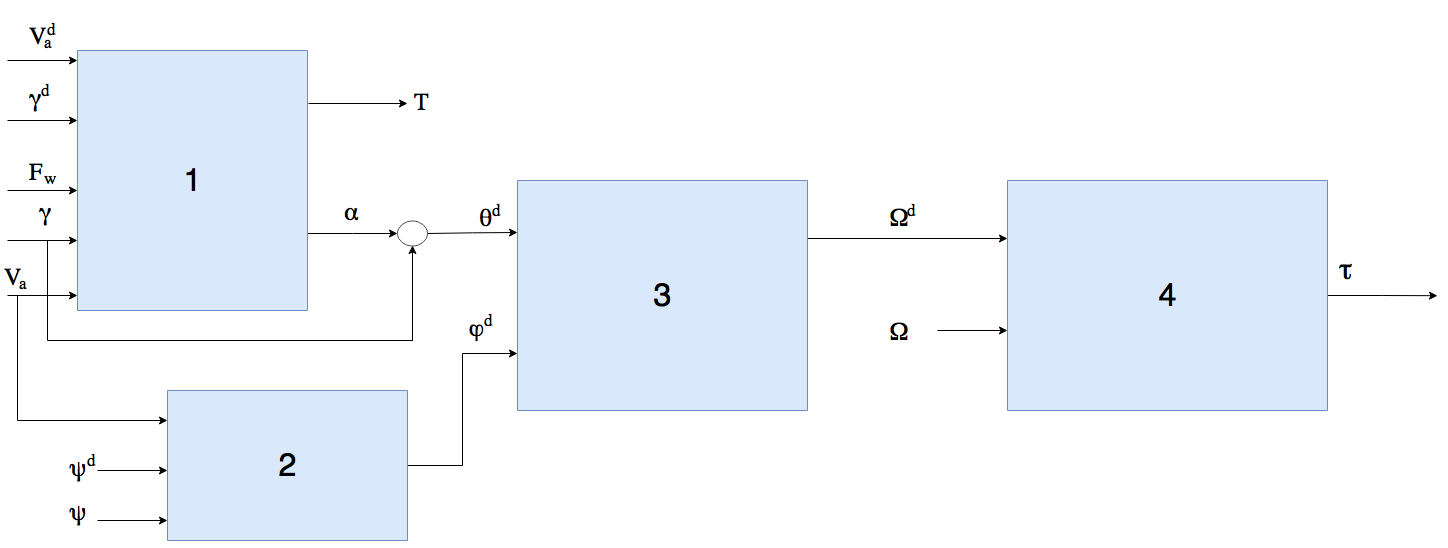
\includegraphics[width=1\textwidth]{Figures/slow_inversion.png}
  \caption[Slow dynamics controller]{This block diagram describes the method used to compute $\tau$, the pseudo input to the fast dynamics inversion. In block \textbf{1} equations \ref{eq:va_dot_des}, \ref{eq:gamma_dot_des}, \ref{eq:gamma_dot} and \ref{eq:gamma_dot} are solved to compute the desired $\theta^d$ and thrust. Similarly in block \textbf{2} equations \ref{eq:psi_dot_des} and \ref{eq:psi_dot} are also solved to obtain $\phi^d$. From these values in block \textbf{3} go through the PD controller described in equatio \ref{eq:omega_PD}, resulting in $\Omega^d$, the input of block \textbf{4}. This last block is the linear controller described by equation \ref{eq:linear_controller}, which output $\tau$.}
  \label{fig:slow_inversion}
\end{figure}

\subsection{Guidance Law}

The final step of the controller design will be to propose a guidance law to obtain the values of $V_a^d$, $\gamma^d$ and $\psi^d$ from the X,Y and Z reference values along time. For these laws it was assumed that the position reference was given relative to a frame of reference with the origin on the Earth surface, with the $Z$ axis pointing upwards. The guidance controller therefore implements the following equations, assuming the errors $\delta x = x_r - x$, $\delta y = y_r - y$ and $\delta z = z - z_r$. The $z$ formula is slightly different to the other two as in the airplane frame of reference the z axis is pointing downwards, allowing this way to use a z reference relative to the Earth surface.

\begin{subequations}
	\begin{gather}
	\delta V_a = \dfrac{1}{\tau_{V_a}}(\sqrt{\delta x^2 + \delta y^2 + \delta z^2})\\
	V_a^d= \delta V_a  + V_{a_0}
	\end{gather}
	\begin{equation}
	\psi^d = atan2(\delta y,\delta x)
	\end{equation}
	\begin{equation}
	\gamma^d = \dfrac{1}{\tau_Z}\delta z
	\end{equation}
	\label{eq:guidance_law}
\end{subequations}

This guidance law is intended to be used having at each time interval a $x_r$, $y_r$ and $z_r$ position of a desired trajectory. These trajectories can be a time parametrized Bezier curve, as per INSERT PAPER FROM HECTOR HERE. From these an airspeed, heading and FPA must be computed and fed to the controller. 
%TODO

Taking first the airspeed equation from \ref{eq:guidance_law}, $V_{a_0}$ is the desired speed of the aircraft in cruise conditions when following the trajectory. This speed is then corrected by the term $\delta V_a$, increasing or decreasing aircraft airspeed depending on its position relative to the trajectory desired position at a given time, i.e the distance error. By dividing this error by $\tau_{V_a}$, a desired convergence time, the speed correction to the initial value $V_{a_0}$ necessary to follow a 4D trajectory is obtained. A more accurate method of obtaining an airspeed reference from these equations is specified in \ref{eq:speed_guidance}. Also, from the $x$ and $y$ position errors between the aircraft and the current trajectory waypoint the desired heading can also be computed using the $atan2$ function. Finally, the method used to obtain the Flight Path Angle relies on the error between the height of the aircraft and the desired one to compute it. 



Using solely equations \ref{eq:guidance_law} however will not grant optimal results, and may even sometimes cause loss of control of the aircraft. The goal for this 4D guidance law and of this work is to, at any given time, to be at a 3D coordinate point of a trajectory at that time. To do so, the references of speed, heading and flight path angle must be constantly adjusted to reach a 4D reference. Using the equations described previously for the guidance controller, it may happen that the aircraft would "overtake" the trajectory reference, causing the heading reference to increase to either $180^o$ or $-180^o$ and therefore making the aircraft diverge significantly from its original trajectory. To avoid this, the following guidance strategy was used:

\begin{itemize}
\item \textbf{Heading} To prevent the heading reference to excessively grow and make the aircraft do a $180^o$ turn, a small correction code in Simulink was added (see algorithm \ref{alg:psi_correction}) in order to detect large errors between the desired and measured heading, caused by the aircraft "overtaking" its trajectory. In case of large errors, this correction would force the desired heading to be equal to its measured value, thus preventing the aircraft from making large turns. 

\begin{algorithm}[H]
	\KwData{$\Psi$ and $\Psi_d$}
 \KwResult{$\Psi$ command}
 error = $\Psi_d$ - $\Psi$\;
 output = $\Psi_d$\;
 \If{$error> 160º$ or $error< -160º$}{
 output =  $\Psi$}
 
 \caption{$\Psi$ command correction algorithm}
 \label{alg:psi_correction}
\end{algorithm}


\item \textbf{Airspeed} Now that the aircraft no longer does $180^o$ turns when it overtakes the desired trajectory, the desired airspeed must now be adjusted in order to slow down and therefore reach the desired position at the desired time. To do so the guidance law was slightly modified to 
\begin{equation}
V_a^d=\begin{cases}
\delta V_a  + V_{a_0} \quad \text{if} \quad |atan2(\delta y,\delta x)|<90^o\\
\delta V_a  - V_{a_0} \quad \text{if} \quad |atan2(\delta y,\delta x)|>90^o
\end{cases}
\label{eq:speed_guidance}
\end{equation}
\end{itemize}

Finally, the block diagram of the controller described thus far is given by figure \ref{fig:controller_noNN}, in which the linear controller is described in more detail in figure \ref{fig:slow_inversion}, and the plane model in figure \ref{fig:plane_model}.

\begin{figure}[!htb]
  \centering
  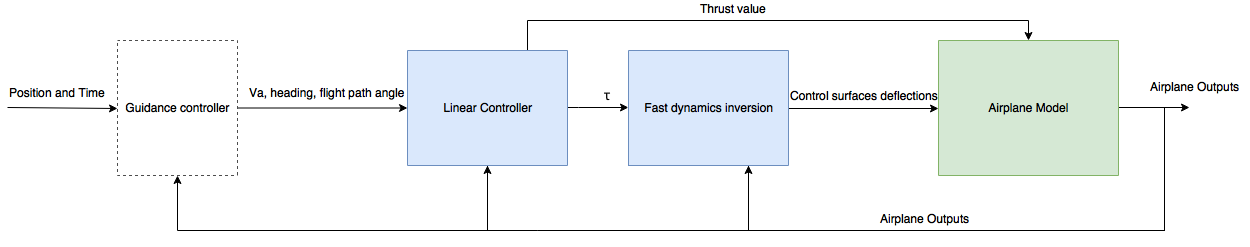
\includegraphics[width=1.15\textwidth]{Figures/controller_noNN.png}
  \caption[Diagram of the controller and model architecture, without NN compensation]{Diagram of the controller and model architecture, without NN compensation}
  \label{fig:controller_noNN}
\end{figure}

\section{Neural Network}
\label{section:NN}

Over the years, intelligent control techniques using neural networks have become a growing research topic, addressing the limitations of state-of-the-art model based controllers such as linear quadratic Gaussian, model predictive control, backstepping and gain scheduling \citep{SotA_IFCS}. Indeed, variations in the plane dynamics (e.g., due to payload changes, actuator or sensor degradation) deteriorate the error of the controller. To compensate for such errors, adaptive online neural networks have been studied and implemented in several works \cite{quad_NLI+NN}, \cite{NN_PID}, \cite{UAV_adaptive} and \cite{NN_NLI} to name a few. These however, have been applied almost exclusively to UAV aircraft, especially multicopters. For this work a feedforward network with one hidden layer (one of the most widely implemented neural network architecture \cite{SotA_IFCS}) was used.


\subsection{Network Architecture}
From an error-less nonlinear inversion, the pseuso-input $\tau$ would directly control $\ddot{\Omega}$ as it was seen previously. However, in case of inversion errors, that can be caused by several factors such as modelling errors or external disturbances, resulting in an equation similar to \ref{eq:system+error}, that $\tau = \ddot{\Omega}^d + \Delta$, where $\Delta = \ddot{\Omega}- \ddot{\Omega} ^d$. This method adds an adaptive component $\tau_{NN}$ to the pseudo input that will approximate the behaviour of the $\Delta$ error. The resulting control law will be given by $\tau + \tau_{NN} = \ddot{\Omega}^d + \Delta$, in which as $t \rightarrow \infty$, $\tau_{NN} \rightarrow \Delta$, thus adaptively minimizing inversion errors. To do so a simple neural network architecture was chosen: a network with a single hidden layer with therefore two sets of weights $V$ and $W$ that will need to be trained, corresponding to the input weights and the hidden layer ones. As for the activation functions for the hidden layer a sigmoid function was chosen, $sig(x)=\dfrac{1}{(1+e^{-x})}$. As the outputs must not be bound between $[0;1]$, the chosen output function was a linear one. Indeed sigmoid output functions are usually used in applications where the output must be a boolean value. A description of the chosen architecture can be found in figure \ref{fig:NN}. Different numbers of neurons were used and the results obtained will be discussed in chapter \ref{chapter:results}.

\begin{figure}[!htb]
  \centering
  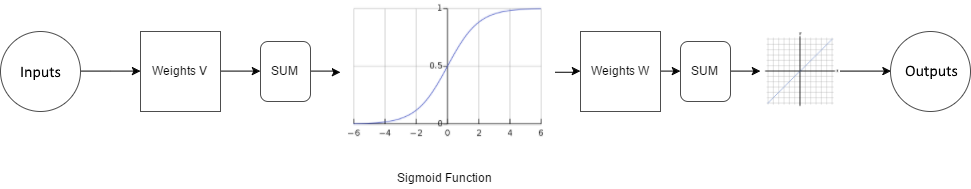
\includegraphics[width=1\textwidth]{Figures/NN.png}
  \caption[Neural Network diagram]{Neural Network diagram}
  \label{fig:NN}
\end{figure}

There are quite some challenges in designing a feed forward neural network. Besides choosing the number of layers and neurons per layer, the inputs of the network must also be chosen carefully. Some rules to choose the correct inputs are given in \cite{NN_inputs}:
\begin{itemize}
\item \textbf{Relevance}: This is the most important consideration to have while choosing inputs, this set must be sufficiently informative of the state of the system for the network to perform correctly. A NN will perform poorly if the output behaviour is not correlated to its input.
\item \textbf{Redundancy}: A large value of redundant and irrelevant input variables will not only increase the needed computational effort of the NN, but will also increase the difficulty to train the weights of the network and add noise to the system.
\end{itemize}

Another consideration about the chosen inputs that must also be taken into account is their range. The sigmoid function $sig(x)$ used reaches around 73\% when $x=1$ and 88\% when $x=2$, as can be seen in figure \ref{fig:sigmoid}. For some cases the inputs might therefore need to be normalized. While this is quite a trivial task in the case of batch training, as the minimum and maximum value of each input is easily obtained before even starting training, such is not the case for online training, and a maximum and minimum value must be proposed \emph{a priori} for each input. The mean of these values should also be close to zero. Should the input not be normalized and reach absolute values much greater than the unity, its activation function output would be constant and the system would therefore not react to input change. This, clearly, is not desirable. To map the input $x$ knowing its minimum and maximum values to its normalized equivalent $y$, the following equation is used

\begin{equation}
y=2\dfrac{x-x_{min}}{x_{max}-x_{min}}-1
\label{eq:normalisation}
\end{equation}

For this  particular case, the state variables of the fast dynamics where used as inputs of the network, namely $\Omega$ and $\dot{\Omega}$.

\begin{figure}[!htb]
  \centering
  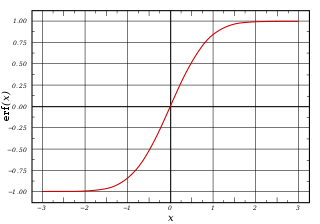
\includegraphics[width=0.5\textwidth]{Figures/sigmoid.png}
  \caption[Sigmoid Function]{Sigmoid Function}
  \label{fig:sigmoid}
\end{figure}

\subsection{Training Algorithm}

As mentioned in section \ref{section:background/NN}, a backpropagation algorithm was used to train both sets of weights online. This algorithm, however, must have an error function that will be minimized by iteratively changing the values of the weights $V$ and $W$. As seen previously, an inversion error $\Delta$ will be present, where $\tau = \ddot{\Omega}^d + \Delta$. This error must be computed for each iteration to train the network to approximate this error. The error can be expressed as $\Delta=\tau - \ddot{\Omega}^d$.
From the control law used to obtain $\tau$ (\ref{eq:linear_controller}) it comes that
\begin{equation}
\Delta = -K_P(\Omega-\Omega^d)-K_D(\dot{\Omega}-\dot{\Omega}^d)
\label{eq:inversion_error}
\end{equation}
Finally the cost function used to train the network is given by

\begin{equation}
J=\dfrac{1}{2}(\Delta-y_{NN})^2
\label{eq:NN_cost}
\end{equation}

The values of $\dot{V}$ and $\dot{W}$ must now be computed, using the gradient descent method described in section \ref{section:background/NN}. As the name suggests, the back propagation algorithm first computes the weight update values for the last layers, propagating the errors to update the previous weight set. The weights are constantly updated until the error absolute value in lesser than a given value $\Delta_{max}$, in which case these are kept constant as $\dot{V}=\dot{W}=0$. 

One of the parameters that must be tuned that has the largest impact on the performance of the network is the learning rate $\alpha$. This coefficient can also be thought of as the step size in incrementing the weight sets. Let $V^*$ and $W^*$ be the two ideal set of weights that, for a given input, result in an absolutely minimal cost function. A small value will allow the weights to converge to their ideal value, although taking many iterations to do so. A large learning rate however might converge faster, but might also overshoot and miss its optimal value. The results of the variation of this rate will be studied in chapter \ref{chapter:results}.

Finally, adding the online neural network to the baseline controller, the final control architecture is obtained. For the following chapter, the controller without the correction will be tested and compared in the same conditions to the same controller including the network. A simplified diagram of the full system, (controller, model and neural network), can be seen in figure \ref{fig:full_controller}.
\begin{figure}[!htb]  
  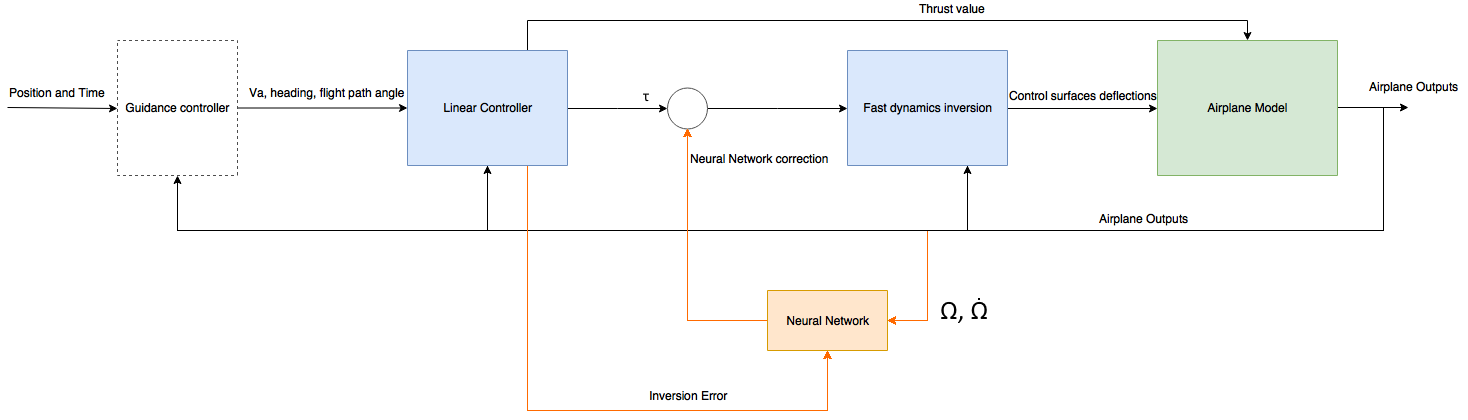
\includegraphics[width=1.1\textwidth]{Figures/full_controller_special.png}
  \caption[Diagram of the controller architecture]{Diagram of the controller architecture including NN correction (in orange)}
  \label{fig:full_controller}
\end{figure}
 % file "Thesis_Implementation.tex"
\cleardoublepage

%\input{Thesis_new_file} % add new .tex files for new chapters
% \cleardoublepage

%\input{Thesis_new_file} % add new .tex files for new chapters
% \cleardoublepage

%\input{Thesis_new_file} % add new .tex files for new chapters
% \cleardoublepage

%%%%%%%%%%%%%%%%%%%%%%%%%%%%%%%%%%%%%%%%%%%%%%%%%%%%%%%%%%%%%%%%%%%%%%%%
%                                                                      %
%     File: Thesis_Results.tex                                         %
%     Tex Master: Thesis.tex                                           %
%                                                                      %
%     Author: Andre C. Marta                                           %
%     Last modified :  2 Jul 2015                                      %
%                                                                      %
%%%%%%%%%%%%%%%%%%%%%%%%%%%%%%%%%%%%%%%%%%%%%%%%%%%%%%%%%%%%%%%%%%%%%%%%

\chapter{Results}
\label{chapter:results}

This chapter will be presenting the results in the behaviour of the aircraft for the different solutions proposed to control and stabilise it. Once the goal for the results of this chapter is properly established, the first step will be to validate the model that was implemented. This will be done by controlling the aircraft into cruise conditions using the baseline feedback linearisation error. The effects of disturbances and inversion errors will then be studied regarding their effects in aircraft dynamics. The next step will be to achieve the goal of this thesis and demonstrate the effects of an on-line neural network in reducing the tracking error in the presence of these disturbances. Finally, from the adaptive controller, including the neural network, the guiding law described in chapter \ref{chapter:implementation} in \ref{eq:guidance_law} will be added to follow a given trajectory.


%%%%%%%%%%%%%%%%%%%%%%%%%%%%%%%%%%%%%%%%%%%%%%%%%%%%%%%%%%%%%%%%%%%%%%%%
\section{Model Validation}
\label{section:results/validation}

The goal in this section will be to validate the behaviour of the model in cruise conditions. Assuming cruise conditions comes that

\begin{gather}
	T=D\\
	W=L\\
	L'=M=N=0
\label{eq:cruise_cond}
\end{gather}
In order to verify the model described so far, the required thrust to have cruise conditions will be computed for a given plausible value of $\alpha$. From this point the airspeed of the aircraft can also be computed. The graph of $C_L$ versus alpha was also obtained from its respective neural network, given by \ref{fig:cl_alpha}
\begin{figure}[!htb]
  \centering
  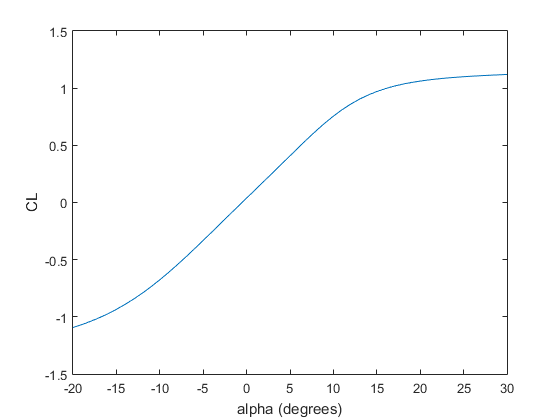
\includegraphics[width=0.75\textwidth]{Figures/CL_alpha.png}
  \caption[$C_L$ versus $\alpha$ graph]{$C_L$ versus $\alpha$ graph from Neural Network}
  \label{fig:cl_alpha}
\end{figure}
From the cruise conditions \ref{eq:cruise_cond}, knowing that $L=\dfrac{1}{2}\rho S V^2 C_L$, solving for the airspeed V comes that

\begin{equation}
V=\sqrt{\dfrac{2mg}{\rho S C_L}}
\label{eq:cruise_speed}
\end{equation}
The required thrust can also be computed from both \ref{eq:cruise_cond}, \ref{eq:cruise_speed} and \ref{eq:cd_cl}, knowing the $C_L$ for a given angle of attack. Proposing some values of $\alpha$, the following results are obtained

\begin{table}[htbp]
  \centering
  \caption{Required cruise conditions for different values of $\alpha$}
    \begin{tabular}{ccccc}
    \toprule
    $\alpha (^o)$ & $C_D$ & $C_L$ & $V (ms^{-1})$ & $T (N)$ \\
    \midrule
    0     & 0.017677131 & 0.0387 & 707.4010791 & 224047.3585 \\
    2     & 0.019379779 & 0.1859 & 322.7613368 & 51133.84325 \\
    4     & 0.023345134 & 0.334 & 240.7952785 & 34283.79709 \\
    6     & 0.029604436 & 0.4828 & 200.279994 & 30076.58604 \\
    \bottomrule

    \end{tabular}
  \label{tab:cruise_cond}%
\end{table}%

From these values, to test both the model (as well as the methods used to simulate the dynamics of the aircraft, including the coefficients neural networks)and the feedback linearisation controller, the following reference values $V_a^d=200 ms^{-1}$, $\gamma^d = 0 rad$ and $\psi^d=0 rad$ were used in an attempt to simulate cruise conditions. From there the values of thrust and angle of attack were computed and  compared to the theoretical values of table \ref{tab:cruise_cond}. 
Following these constant reference values the results obtained were

\begin{figure}
\centering
\begin{minipage}{0.49\textwidth}
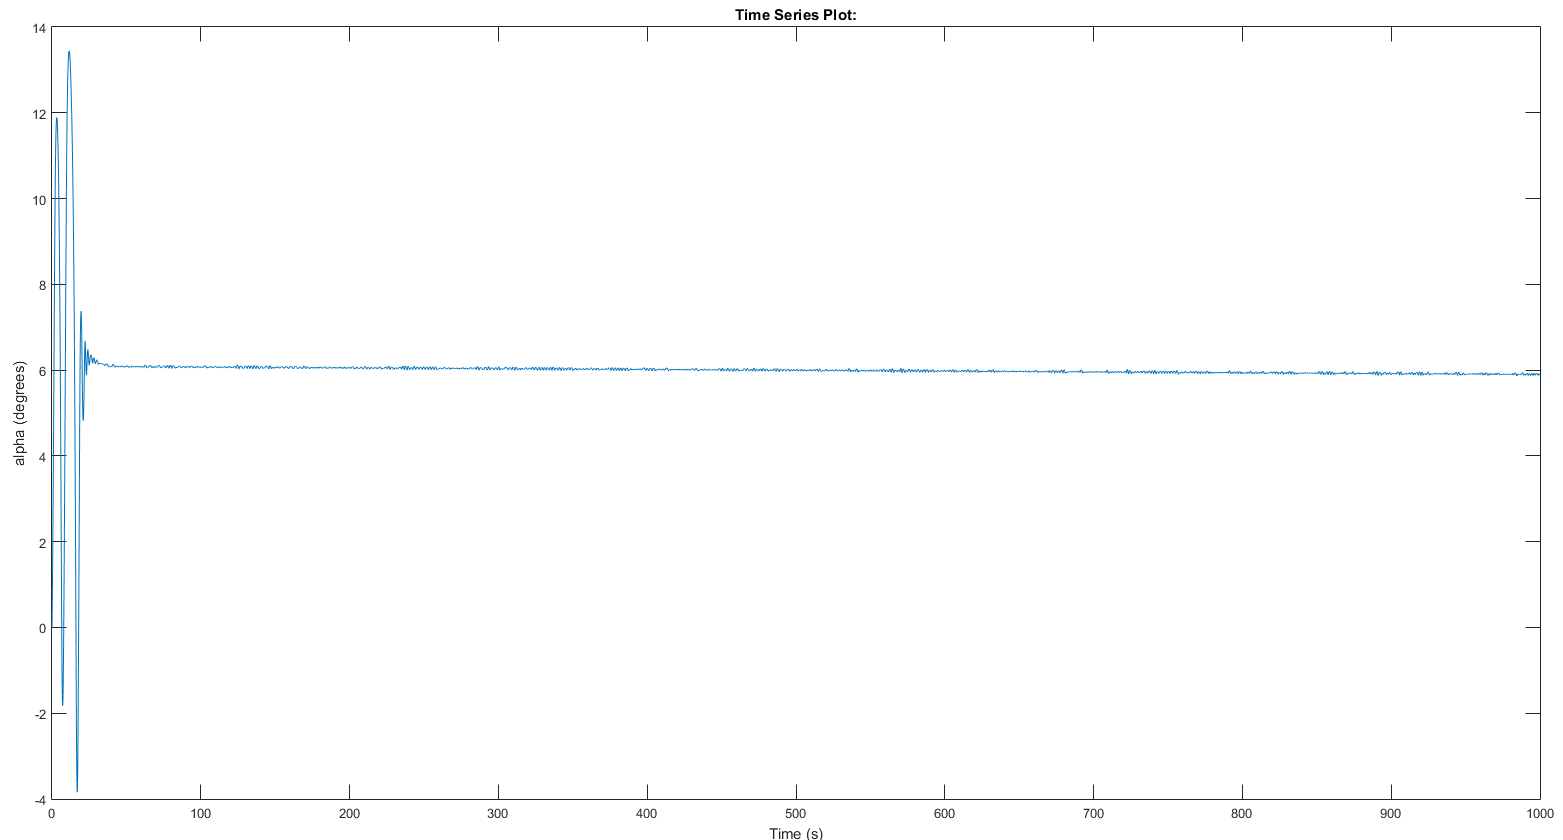
\includegraphics[width=\textwidth]{Figures/Results/aoa_check.PNG}
\end{minipage}
\begin{minipage}{0.49\textwidth}
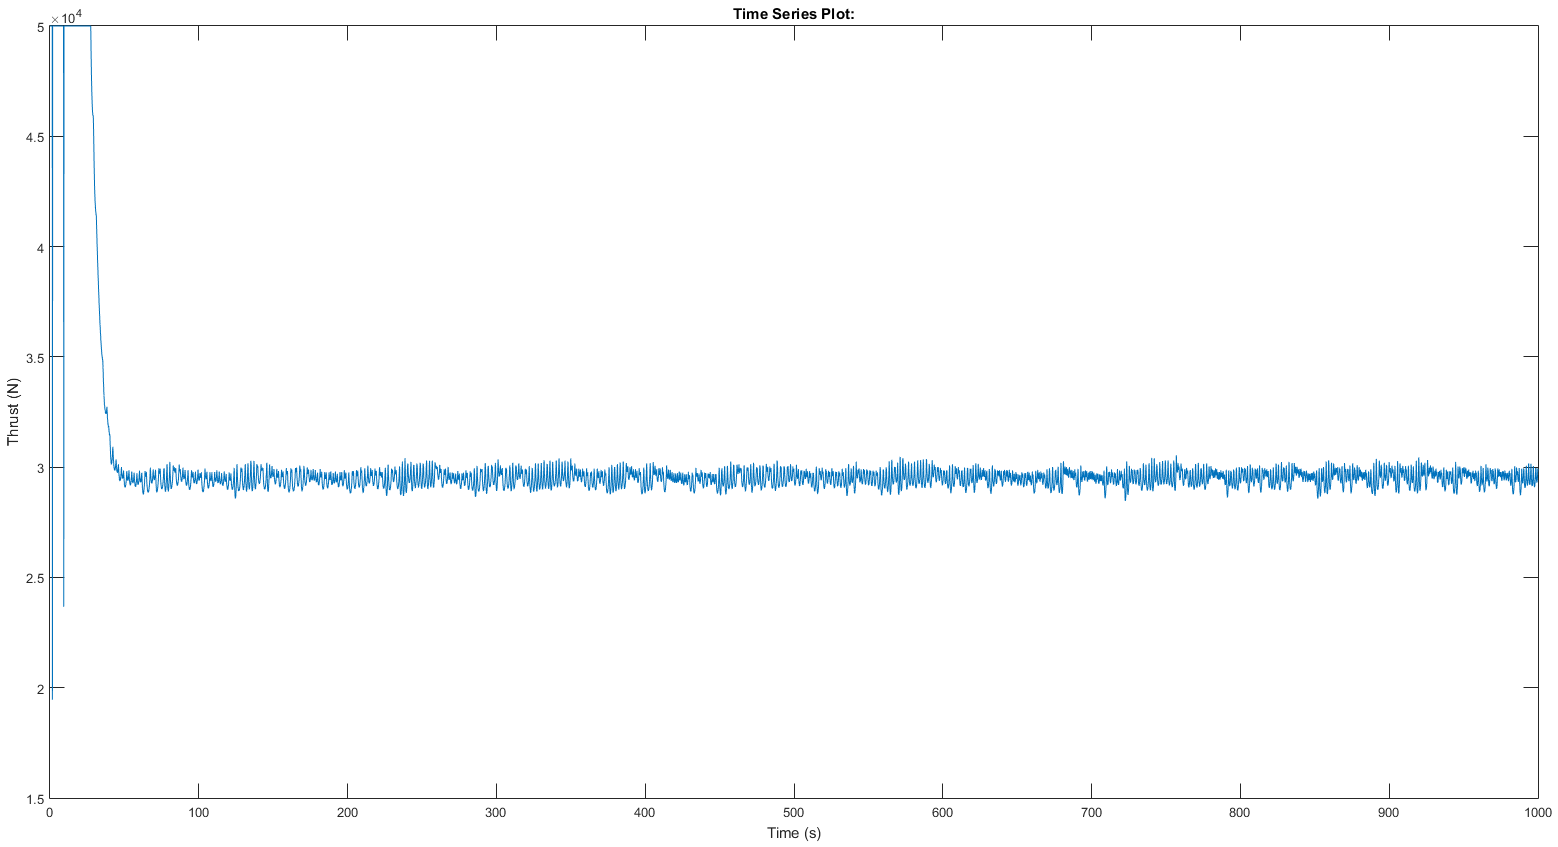
\includegraphics[width=\textwidth]{Figures/Results/thrust_check.PNG}
\end{minipage}
\caption[AoA and thrust validation]{Angle of Attack (degrees) and thrust (N) of the controlled aircraft}
\end{figure}

This simulation, made over 800 seconds, shows clearly that the angle oscillates around a $6^o$ degree angle of attack, with an amplitude of around $0.4^o$ degrees. As for the thrust, it also oscillates around $30000N$ with an amplitude of $2000N$. These values correspond to the theoretical values in table \ref{tab:cruise_cond} for $\alpha=6^o$, indicating that not only the modelled plane is well behaved, but also that the coefficient neural networks are able to simulate an accurate model of the aerodynamic coefficient's variation.


%%%%%%%%%%%%%%%%%%%%%%%%%%%%%%%%%%%%%%%%%%%%%%%%%%%%%%%%%%%%%%%%%%%%%%%%
\section{Feedback linearisation controller}
\label{section:results/fl_contro}

Once the model has been tested and validated, the described nonlinear inversion controller can now be tested. Reference tracking will firstly be observed with simple constant reference values, without any guidance control law. Reiterating the example from the previous section in cruise conditions for $V_a^d=200 ms^{-1}$, $\gamma^d = 0^o$ and $\psi^d = 0^o$ comes that
\begin{figure}[h]
\centering
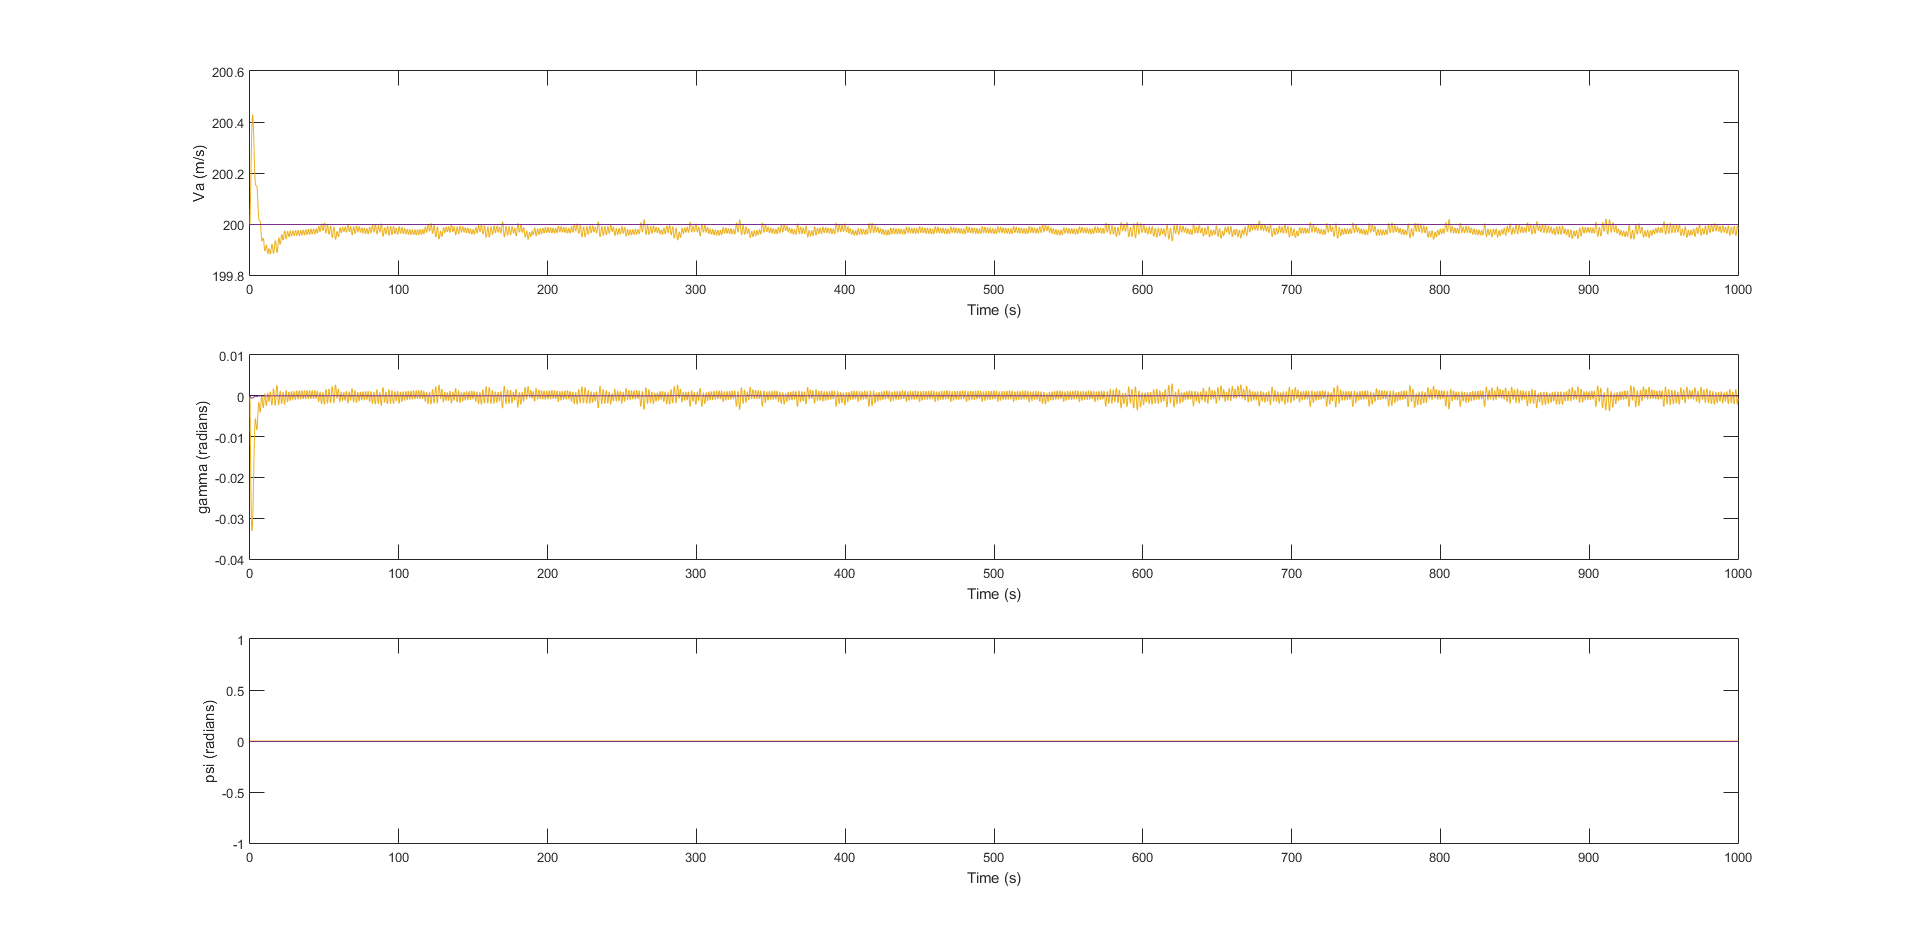
\includegraphics[width=\textwidth]{Figures/Results/nli_test_const.png}
\caption[Constant reference following of feedback linearisation controller]{Reference (blue) following over $1000s$ of simulation time for $V_a^d=200 ms^{-1}$, $\psi^d = 0^o$ and $\gamma^d = 0^o$ respectively and measured values (yellow)}
\label{fig:const_ref}
\end{figure}

As seen in the figure \ref{fig:const_ref} the reference is followed with minimal osculations for the three variables, although with the presence of some steady state error in the case of the airspeed $V_a$. To be able to follow trajectories however, a good control of the aircraft's heading will be necessary. Proposing this time the following variation in $\psi^d$
\begin{equation}
\psi^d = \begin{cases}
0^o & t < 100\\
90^o & 100 \leq t < 500\\
0^o & t > 500 \\
\end{cases}
\label{eq:test_traj}
\end{equation}

The comparing the measured heading $\psi$ and its desired value comes 
\begin{figure}[h]
\centering
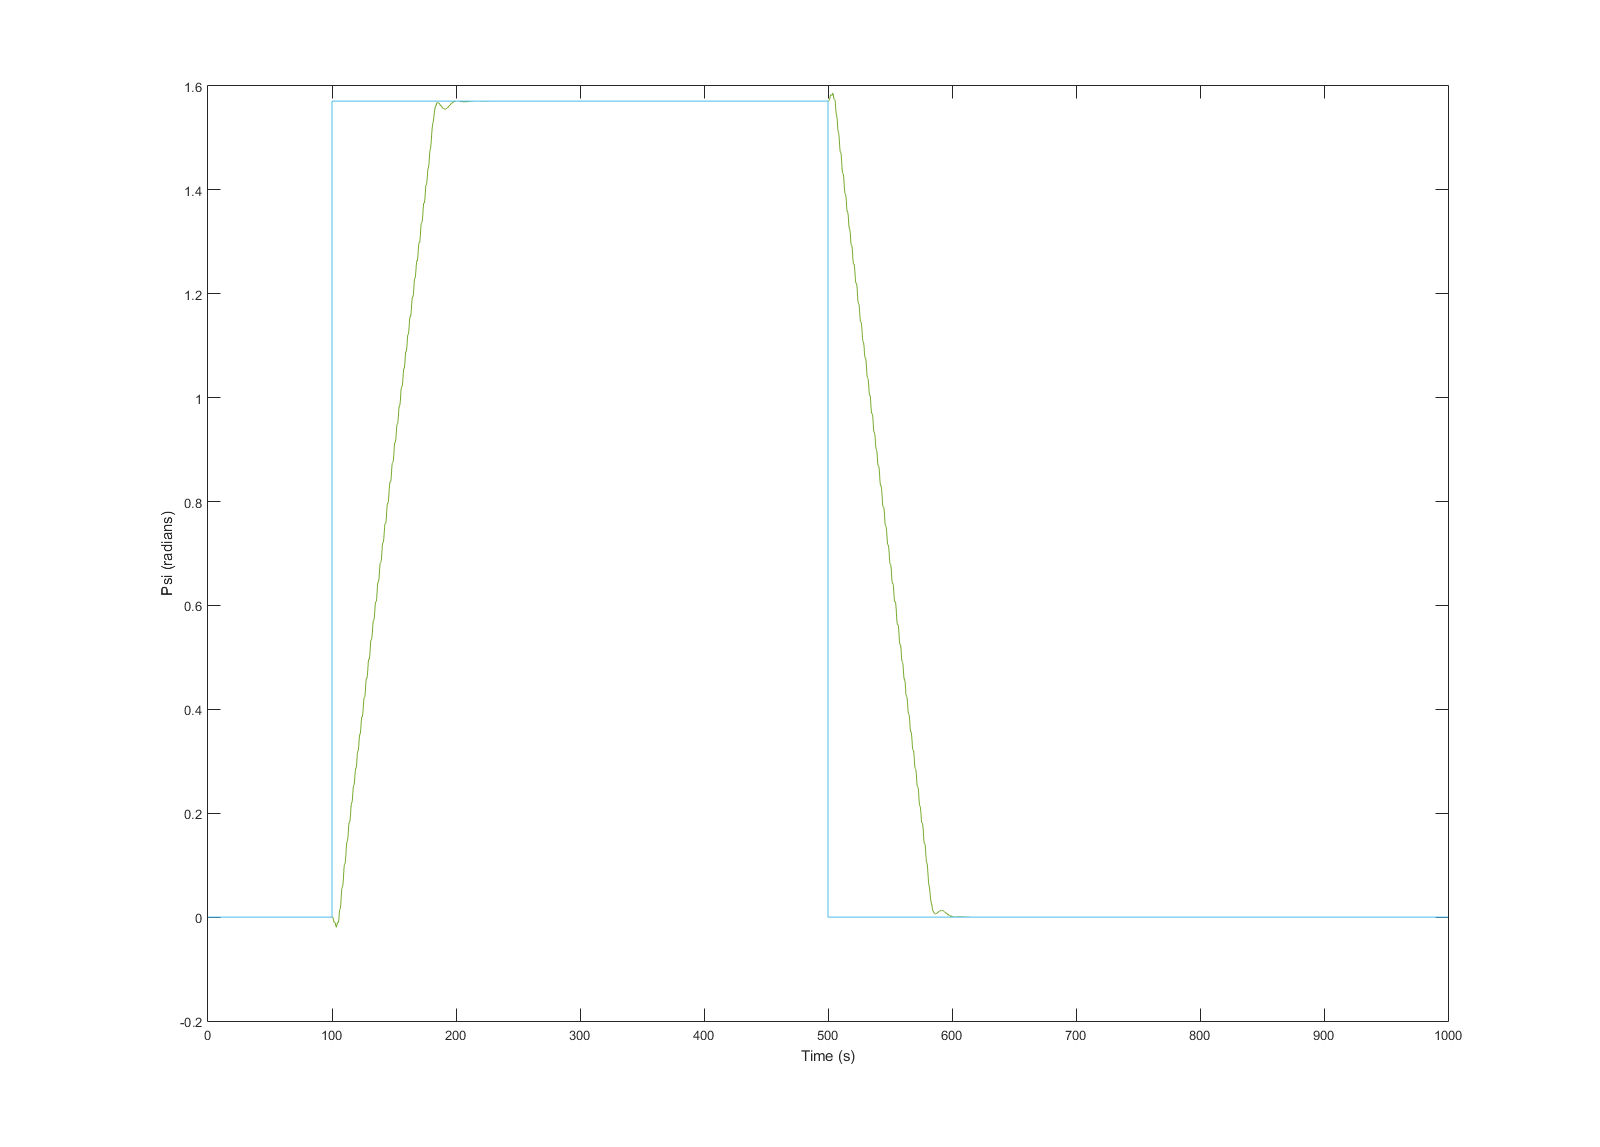
\includegraphics[width=\textwidth]{Figures/Results/heading_test.png}
\caption[Desired and measured heading]{Desired (blue) and measured (green) heading}
\label{fig:heading_test}
\end{figure}

Although the reference value is reached after each step, the convergence takes around $100s$ for a $90^o$ perturbation to converge, without overshoot. These conversion times can be explained by the high inertia and mass of the commercial aircraft. The resulting airplane trajectory can be seen in figure \ref{fig:trajectory}.

\begin{figure}[h]
\centering
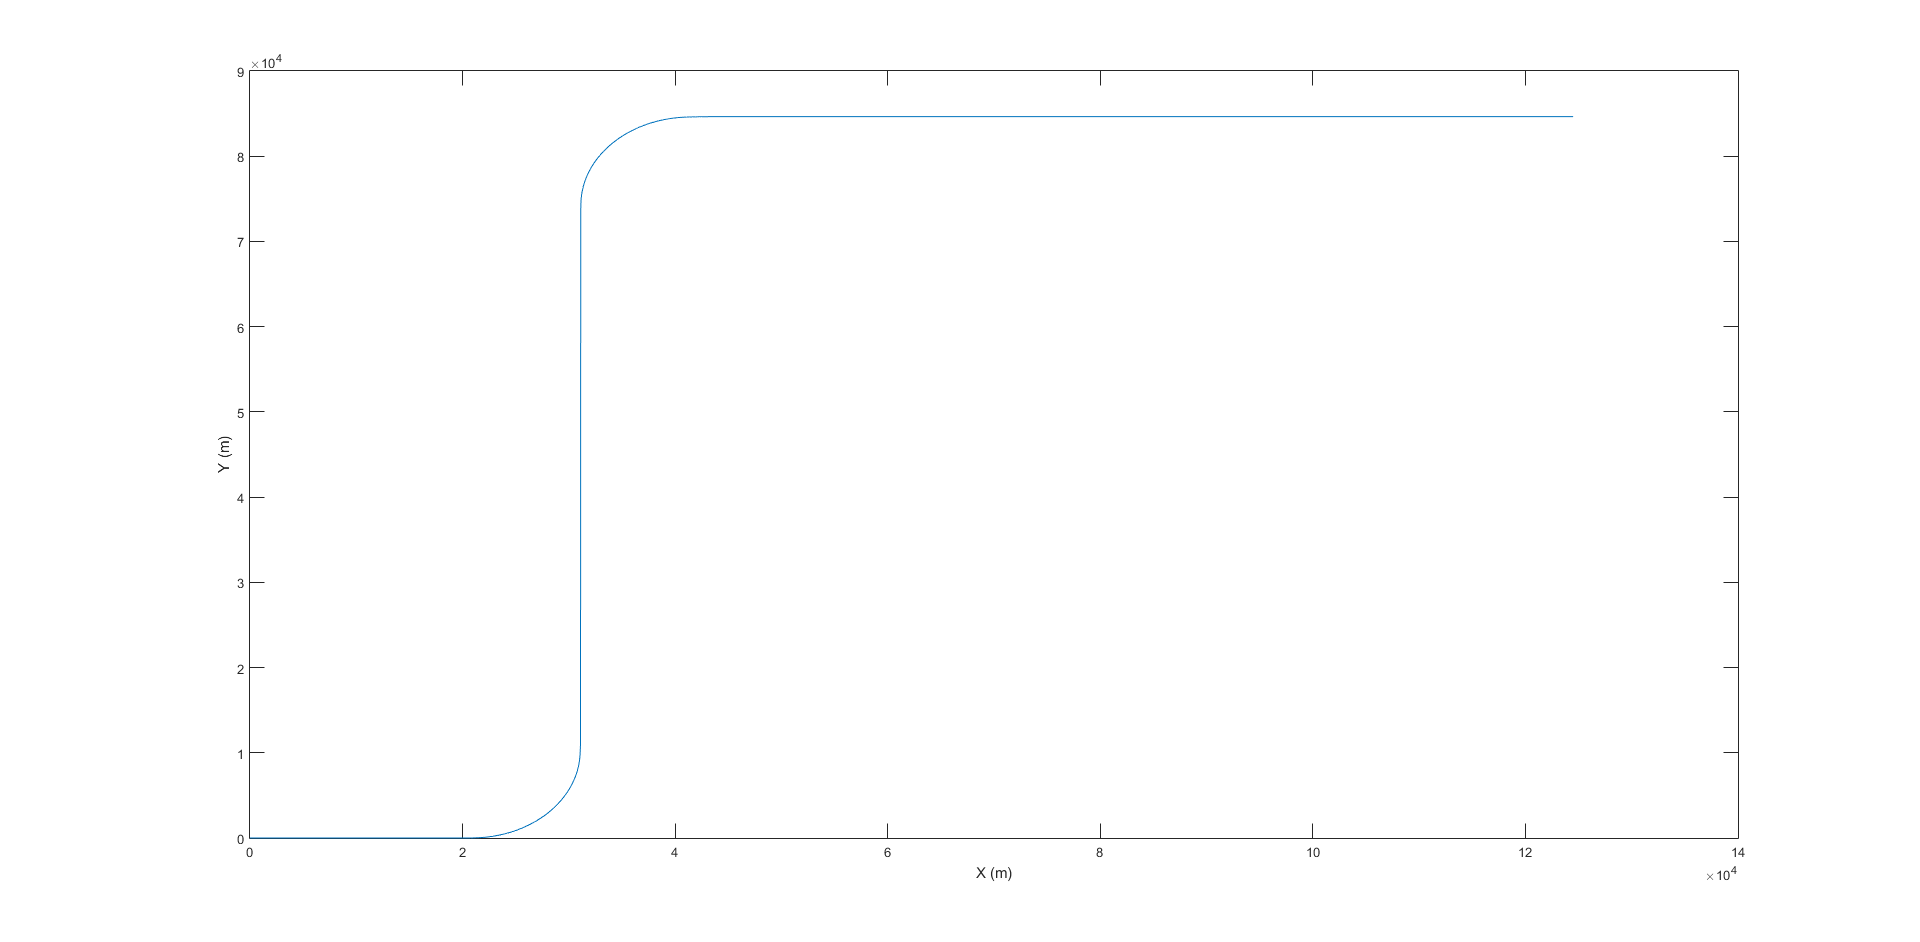
\includegraphics[width=\textwidth]{Figures/Results/trajectory.png}
\caption[Plane trajectory]{Plane trajectory for the mention control input}
\label{fig:trajectory}
\end{figure}

\section{Disturbances and Errors}
\label{section:results/disturbances_errors}

From the results obtained in the previous section, it can be concluded the controller performs correctly following the desired reference. These results however were obtain supposing the exact model of the aircraft was known, without any kind of external perturbation or simulated system failure. It is these perturbations that will be simulated in this section and studied. To do so the same testing reference as described in equation \ref{eq:test_traj} will be used to compare the effects of different types of disturbances with the undisturbed system. 

\subsection{Inversion errors}

This error will be the most frequent when implementing such a controller, as some system parameters estimations may have considerable errors, namely the aircraft's inertial matrix. Fortunately, the controller used is, as will be demonstrated, tolerant to errors in the estimation of this parameter, but can result in an unstable system in extreme cases. To simulate estimation errors, the entries of the inertial matrix $A$,$B$,$C$ and $E$ were multiplied by a reducing factor $\zeta \in [0;1]$ when computing the nonlinear inversion in \ref{eq:control_law}. The inertial matrix used in this equation $I_{est}$ is therefore given by $I_{est} = \zeta I$.

Changing the values of $\zeta$ to $0.5$ and $0.05$, increasing the inversion error, results in the following trajectories in figure \ref{fig:inversion_error}

\begin{figure}[H]
\centering
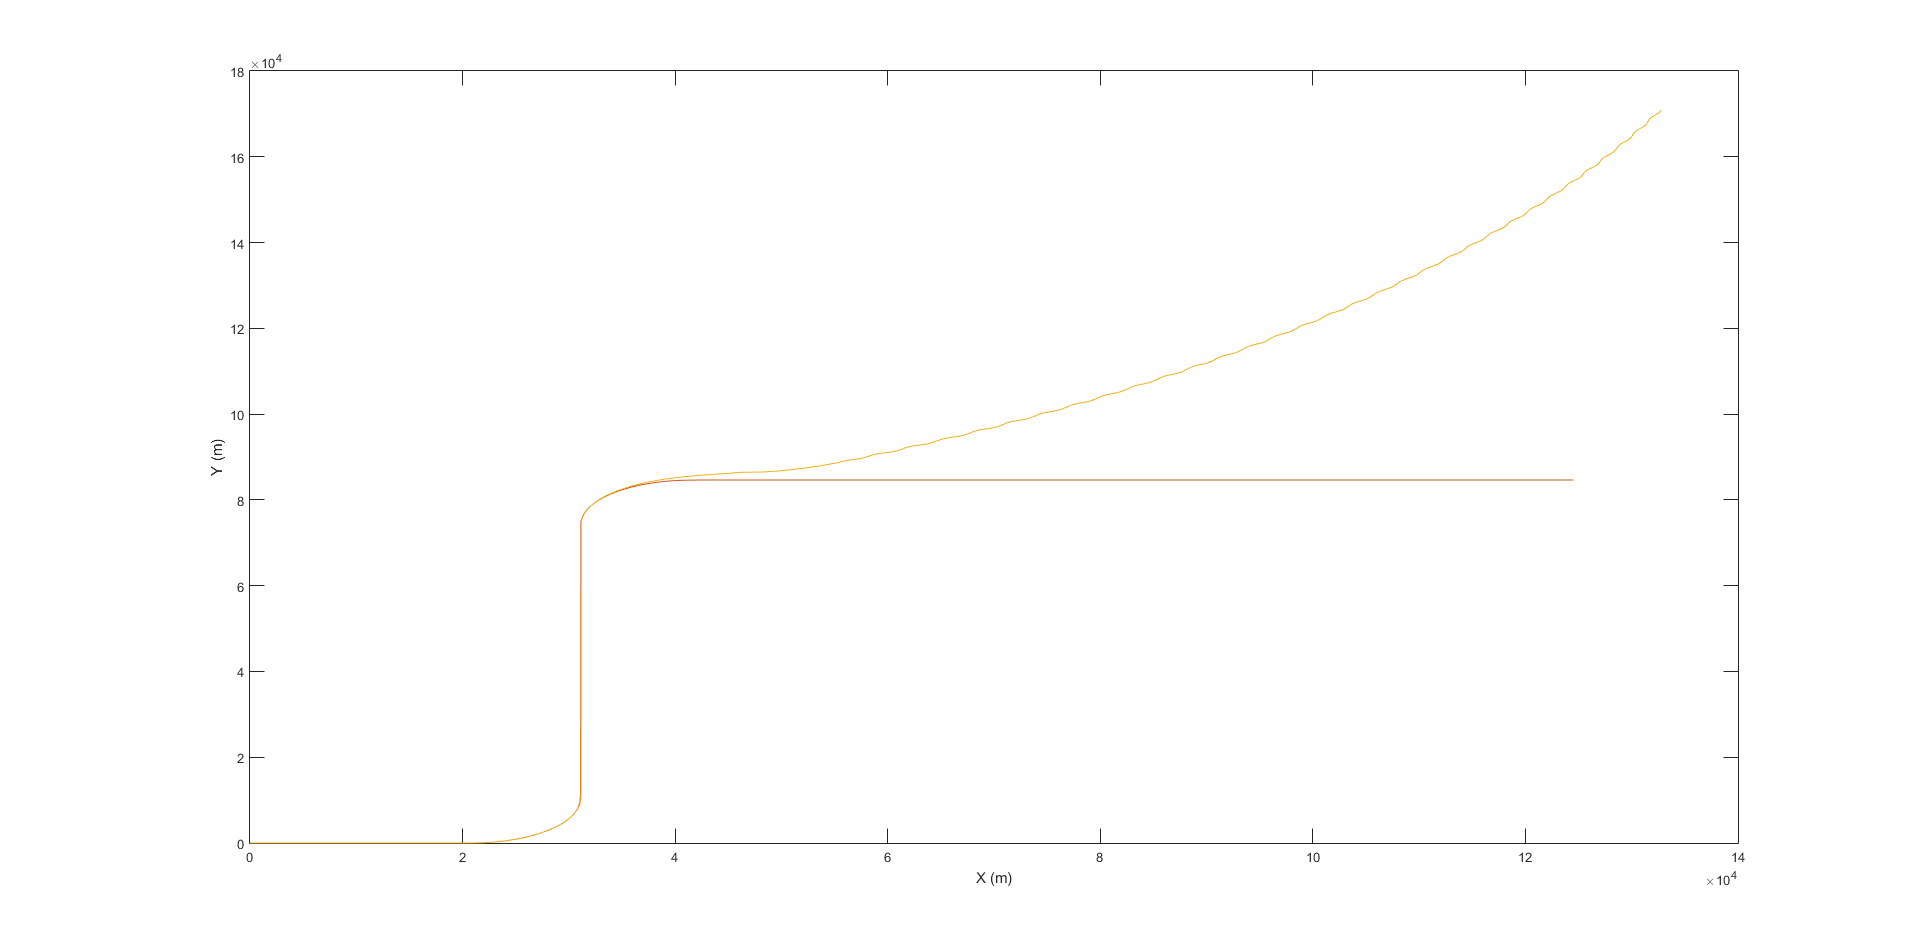
\includegraphics[width=\textwidth]{Figures/Results/inversion_error.png}
\caption[Plane trajectory with inertia estimation errors]{Plane trajectory for for $\zeta = 0.5$ (red) and $\zeta= 0.05$ (yellow)}
\label{fig:inversion_error}
\end{figure}

Indeed, a 50\% error in estimating the inertia of the aircraft when computing the feedback linearisation law results in a negligible reference tracking error, as can be seen in figure \ref{fig:ref_zeta_05}. This however is not the case if $\zeta$ is reduced even further to $\zeta = 0.05$ and error of the system relative to its references becomes much greater (figure \ref{fig:ref_zeta_005}. As can be seen in this figure, the aircraft is unable to follow yaw commands in this case as it easily goes unstable. This establishes a first goal to measure the performance of the designed neural network, to try to approach the case of $\zeta = 0.05$ to the reduced errors of a nonlinear inversion with no inertia estimation errors.

\begin{figure}[H]
\centering
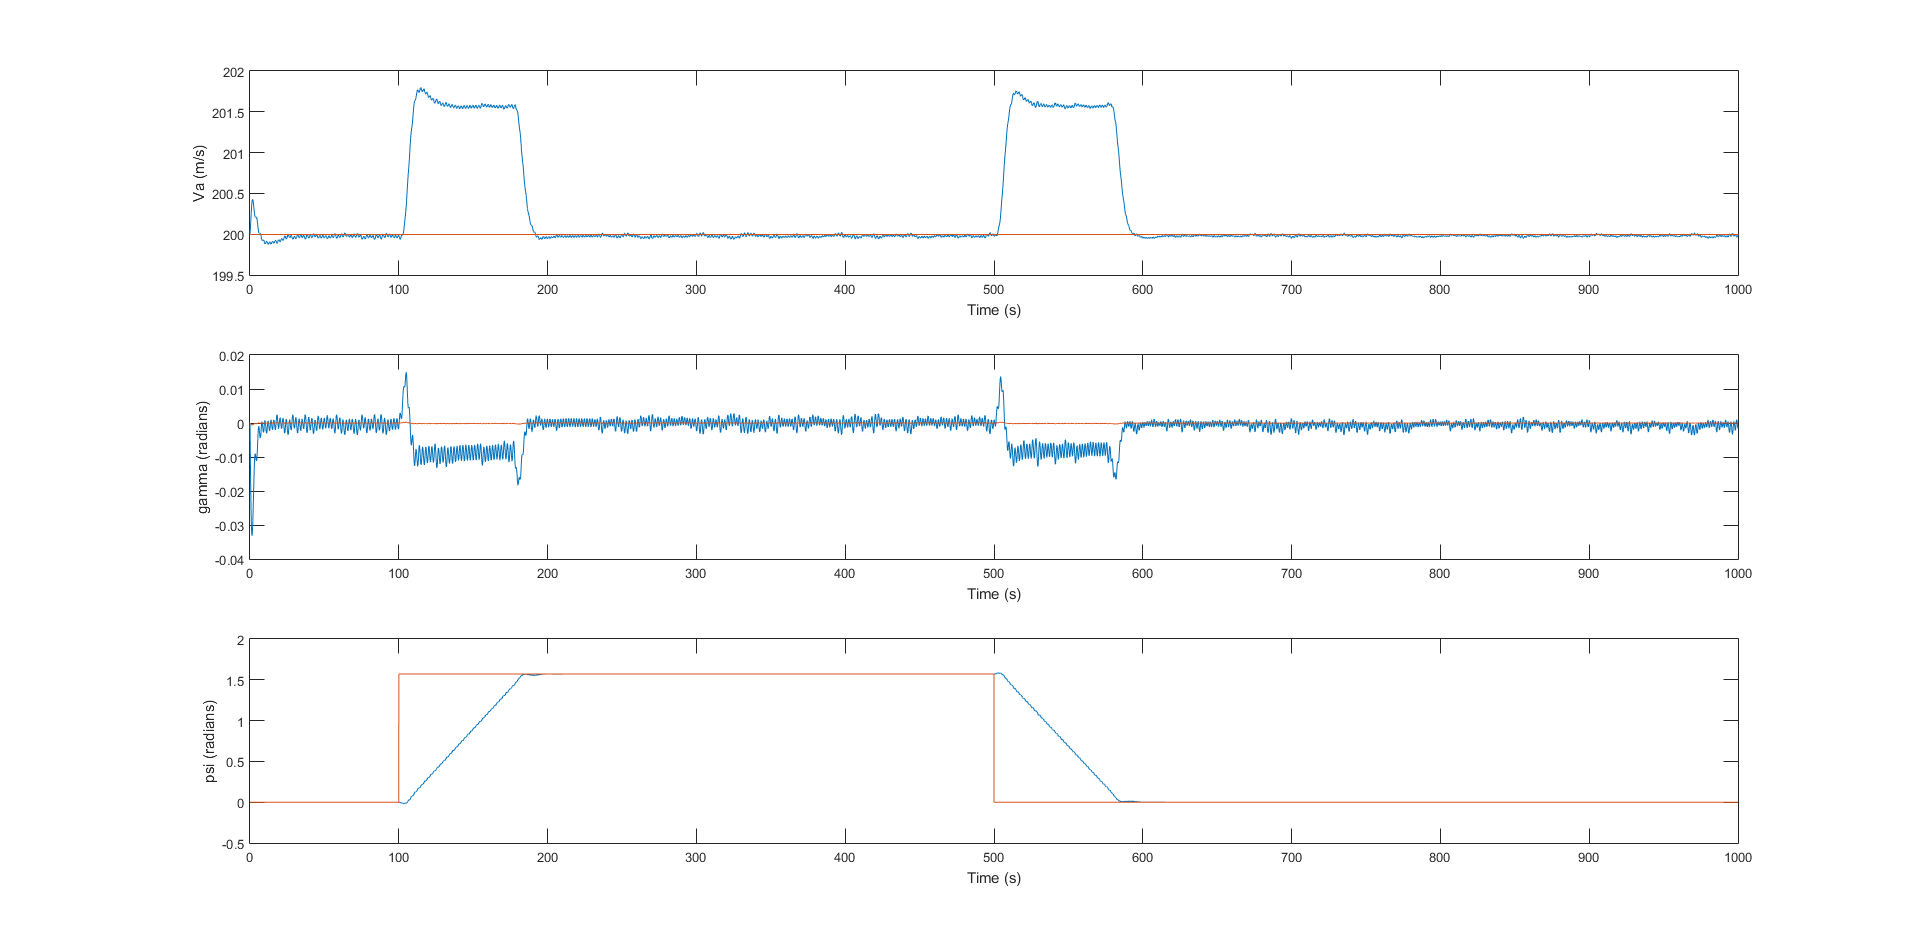
\includegraphics[width=\textwidth]{Figures/Results/ref_zeta_05.png}
\caption[Reference tracking for $\zeta=0.5$]{$V_a$, $\gamma$ and $\psi$ for measured and desired values for $\zeta=0.5$}
\label{fig:ref_zeta_05}
\end{figure}
\begin{figure}[H]
\centering
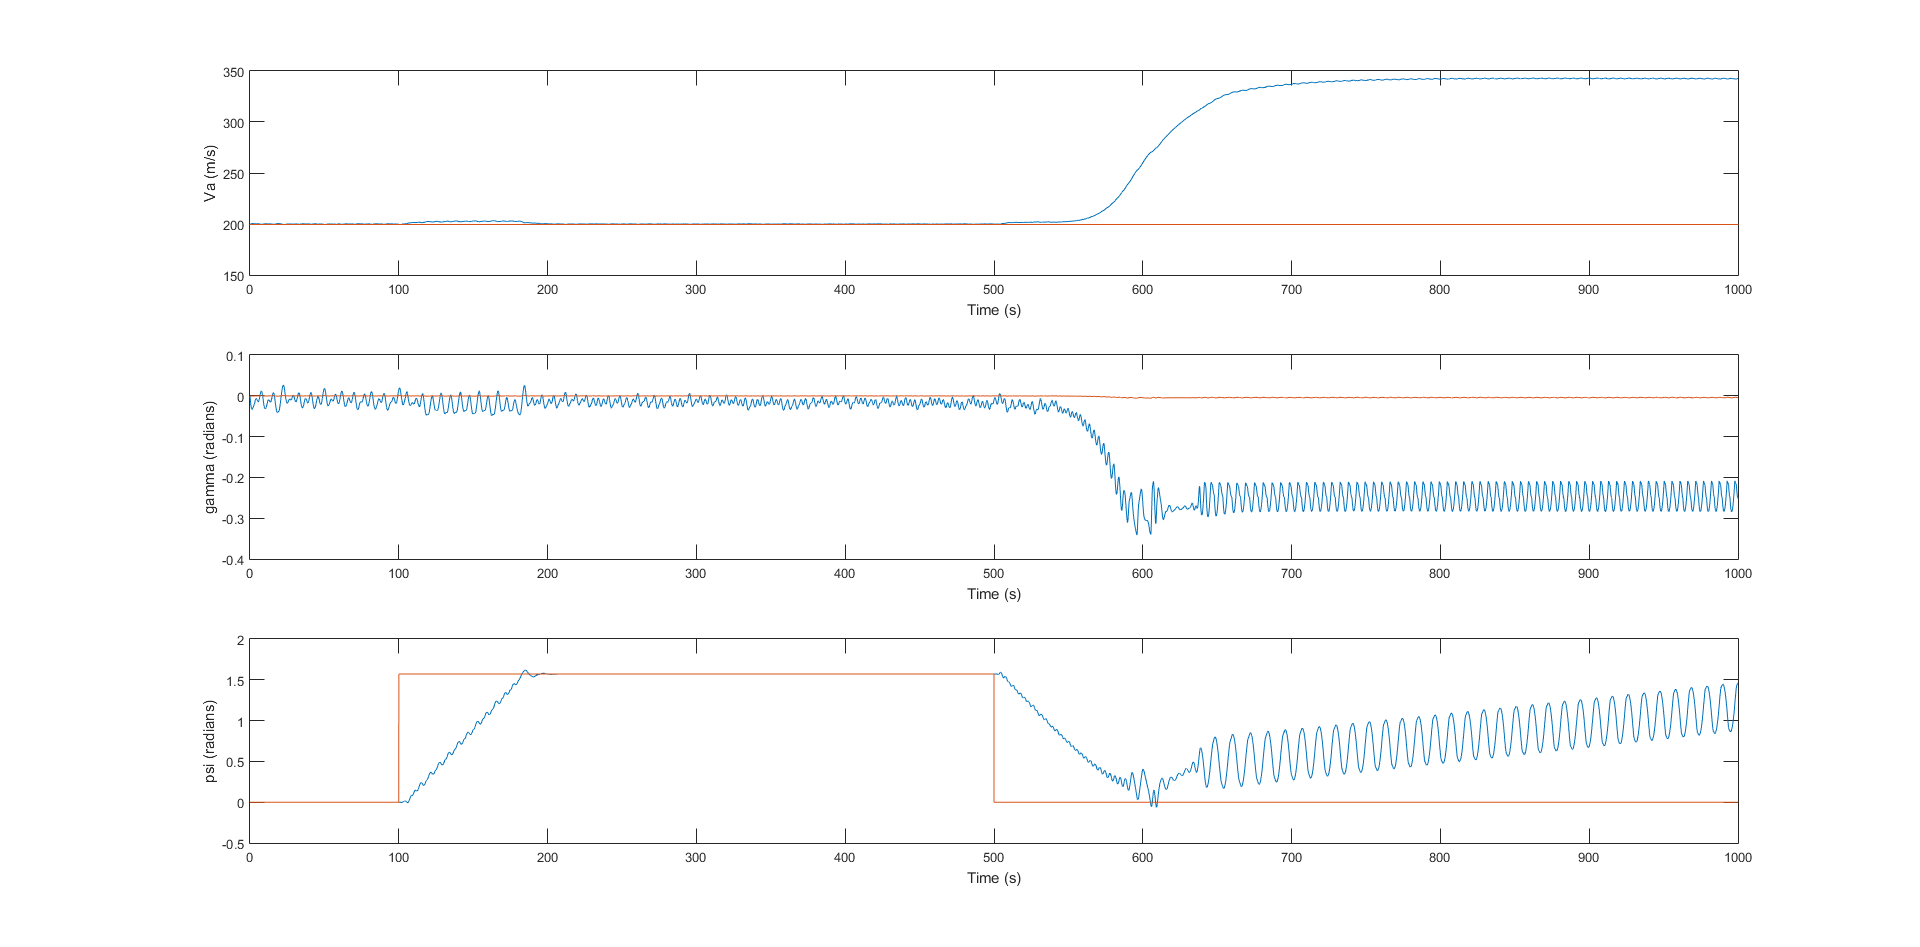
\includegraphics[width=\textwidth]{Figures/Results/ref_zeta_005.png}
\caption[Reference tracking for $\zeta=0.05$]{$V_a$, $\gamma$ and $\psi$ for measured and desired values for $\zeta=0.05$}
\label{fig:ref_zeta_005}
\end{figure}

\subsection{System failures}

One other cause for inversion errors that can have a much greater impact on flight trajectory are system failures. This subsection will focus on methods to simulate these failures and observe the behaviour of the airplane trajectory for these cases. The reference trajectory that will be used shall be the same as used previously. The first failure to be simulated will be a control surfaces failure, that will lead to reduced controllability of the aircraft. In this work this was replicated in a simulated environment by reducing each moment coefficients for the elevon, aileron and rudder, namely $C_{\delta_{ele}}$, $C_{\delta_{ail}}$ and $C_{\delta_{rud}}$.

By setting each of these coefficients to 20\% of their initial values, the effect of the errors in followed trajectory become visible in figure \ref{fig:reduced_act}. This figure show that the reduced controllability results in a $20km$ difference to that of the undisturbed system. This sets the second goal for the performance of the neural network, to reduce this error as much as possible.

\begin{figure}[H]
\centering
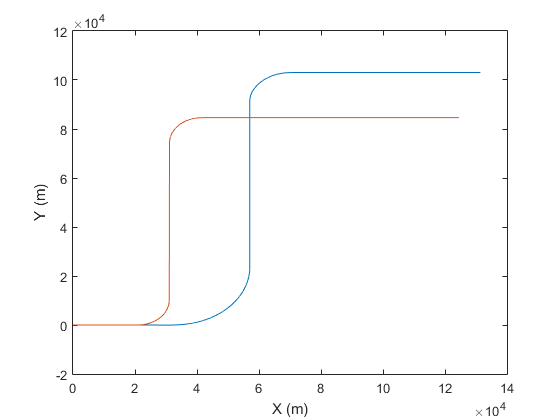
\includegraphics[width=\textwidth]{Figures/Results/reduced_act.png}
\caption[Trajectory with reduced actuation]{Trajectory with 20\% reduced actuation (blue) and trajectory without failures (red)}
\label{fig:reduced_act}
\end{figure}

One second type of flight perturbation that will be included in this subsection is the effects of icing conditions in aircraft flight. According to the FAA guide to flight in icing conditions, ice contamination of an airfoil has an important influence on both the Lift and Drag curves \cite{icing_cond}. Ways to simulate these perturbations in a modelled environment will be studied, and as for the the other described disturbances an online neural network will be used to improve the control of the aircraft in such conditions. The main drawbacks that can be caused by icing are

\begin{itemize}
\item \textbf{Stall }As seen in figure \ref{fig:icing_lift}, ice contamination of the airfoil leads to a significant reduction in the value of the maximum $C_L$, causing the aircraft to reach stall conditions ata much lower angle of attack. Reducing speed (e.g for an approach) makes this effect more noticeable for the pilot. The usual reduction on $C_{L_{max}}$ is of 30\% \cite{icing_cond}.

\item \textbf{Drag }Drag will increase directly with the amount of ice accumulated on the wing, reaching usual values of 100\% of the initial drag coefficient.

\item \textbf{Roll }Icing on the main wings will also affect roll control. As the thickness of the wing decreases towards its tip, so increases its efficiency to collect ice, leading to a partial stall in the tip of the wings, according to the AOPA manual \cite{icing_aopa}.
\end{itemize}
\begin{figure}[H]
\centering
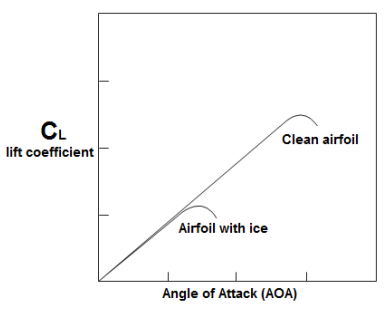
\includegraphics[width=0.7\textwidth]{Figures/Results/icing_lift.PNG}
\caption[Effects of icing on lift coefficient]{Effects of icing on lift coefficient \cite{icing_cond}}
\label{fig:icing_lift}
\end{figure}
\begin{figure}[H]
\centering
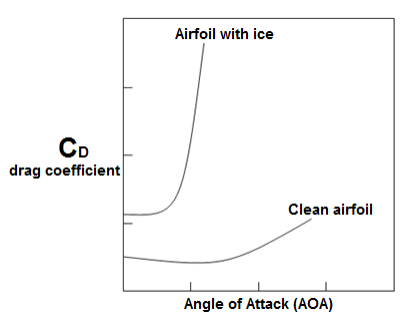
\includegraphics[width=0.7\textwidth]{Figures/Results/icing_drag.PNG}
\caption[Effects of icing on drag coefficient]{Effects of icing on drag coefficient \cite{icing_cond}}
\label{fig:icing_drag}
\end{figure}

Following these indications to simulate heavy icing condition, the lift coefficient $C_{L_{max}}$ was reduced by 30\%, and the stall angle reduced from $15^o$ (see figure \ref{fig:cl_alpha}) resulting in figure \ref{fig:cl_icing}. The value of the drag coefficient was also augmented by 200\% from equation \ref{eq:cd_cl}. Finally, in order to simulate roll control limitations, the value of $C_{\delta_{ail}}$ was reduced by 30\%. These values were chosen in order to deteriorate the control of the aircraft, while allowing for the possibility of reference following without reaching actuator saturation (for both control surface deflections and thrust). 

For this case a sinusoidal yaw reference was given of $\psi^d= 45 \sin (1.1459t)$ degrees, t being the simulation time. A sinusoidal reference was used to make the effects of simulated icing more noticeable, and the same references of $V_a^d=200ms^{-1}$ and $\gamma^d=0$ as previously were used. For this case, the results obtained were, for both icing and non icing conditions,

\begin{figure}[H]
\centering
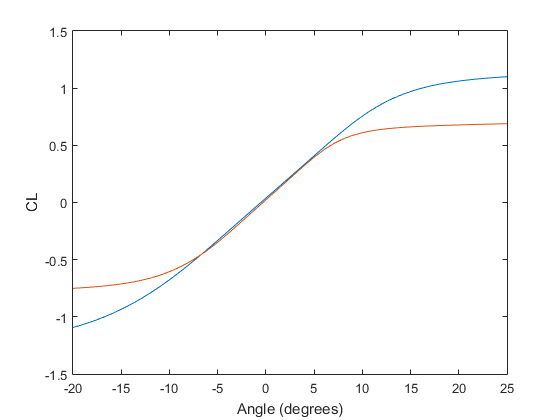
\includegraphics[width=0.5\textwidth]{Figures/Results/cl_icing.PNG}
\caption[Lift coefficient simulation in icing conditions]{Lift coefficient simulation in icing conditions}
\label{fig:cl_icing}
\end{figure}

\begin{figure}[H]
\centering
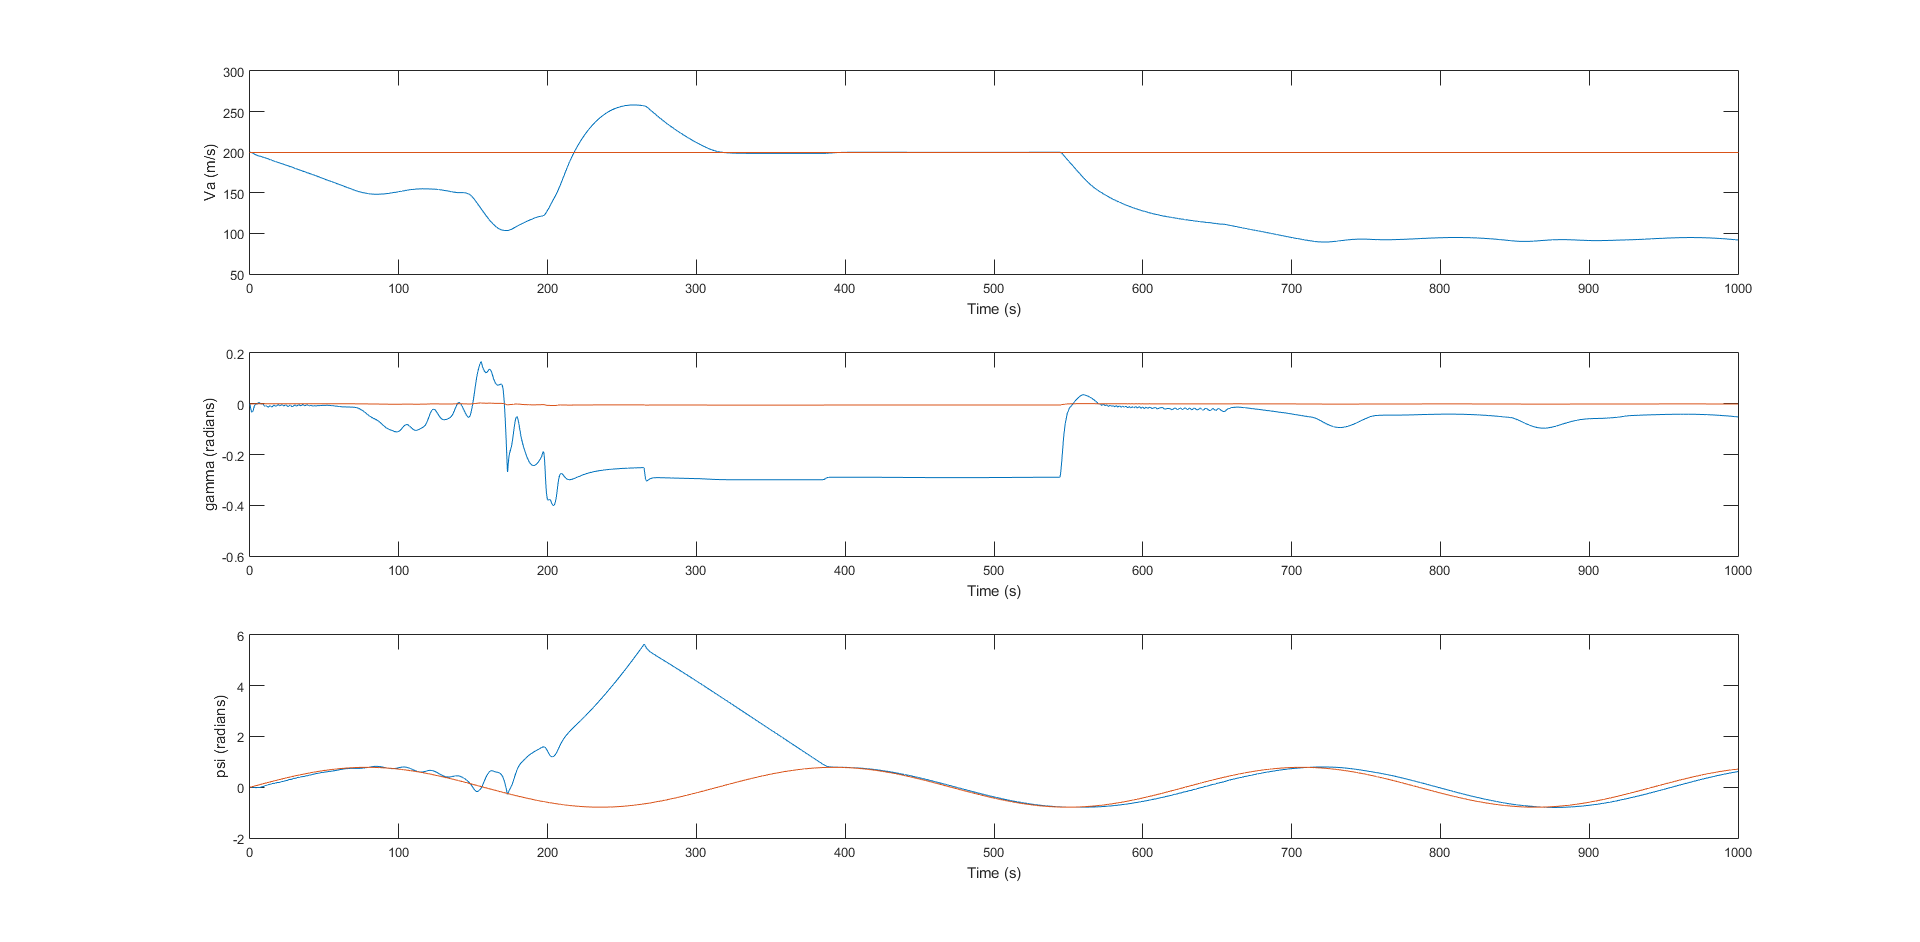
\includegraphics[width=1\textwidth]{Figures/Results/ref_icing.PNG}
\caption[Reference following in icing conditions]{$V_a$, $\gamma$ and $\psi$ for measured and desired values in icing conditions}
\label{fig:ref_icing}
\end{figure}

From figure \ref{fig:ref_icing}, the system in such high drag conditions can be considered marginally stable, as it easily increases the error to either of the three commanded inputs to significantly high values. The impact of the increased drag in noticeable in the reduced speed in the simulation, going under $70ms^{-1}$ for the desired $V_a^d=200ms^{-1}$.

%\subsection{Wind disturbances}

%TODO

These perturbations change the expected behaviour of the aircraft, causing the feedback linearisation control law to perform poorly. In the next section of this work the results of the online neural network will be shown, demonstrating its ability to increase the stability of the aircraft in situations of strong perturbations, or even in cases of a poorly designed linear or feedback linearisation controller. Note however that that the conditions used here to induce the aircraft into unstable or marginally stable conditions mimic extreme perturbations, and the described controller can be said to perform well in cases when little to none of these perturbations are present.


\section{Neural Network}
\label{section:results/NN}

The application of neural networks to improve the overall performance of a controller has been studied for a few years, for different kinds of systems such as multicopters, UAVs and launch based vehicles (\cite{quad_NLI+NN}, \cite{YANG+LIN_Adaptive_Flight_Control}, \cite{NN_PID2}) as well as to improve different types of control laws. These go from simple PIDs in \cite{NN_PID}, \cite{NN_PID2} to  backstepping and nonlinear inversion techniques \cite{NN_backlash} and \citep{NN_NLI}. The applicability of this adaptive control technique has not, however, been studied to commercial aircraft, being usually applied to non manned vehicles. Most of the works that aim to use NN to create an adaptive controller improving upon another control law usually face the similar limitation of needing large amounts of flight data to batch train the network. This work therefore aims to solve this very problem introducing online training based on the backtracking algorithm. 

In the previous section, the simulated controlled aircraft was submitted to conditions that severely limited its correct performance. These will be studied once again, this time using the online NN described in section \ref{section:NN}, comparing the results with the new adaptive component of the control law. The neural network architecture used has a single single hidden layer and used two activation functions, a sigmoid function for the hidden layer output and a linear function for the output of the network, as explained previously. 


\subsection{Inversion Errors}

The first adaptive capability of this method that will be described is the compensation of inversion error due to an incorrect estimation of the plane's inertia. Taking the previous example of \ref{fig:ref_zeta_005}, it can be observed that the aircraft becomes unstable at $t=600s$, leading to a significant increase of airspeed from the desired $200ms^{-1}$ to $350ms^{-1}$. The heading of the aircraft also becomes uncontrollable, oscillating and slowly increasing. 

This is caused due to the $\Delta$ component of equation \ref{eq:inversion_error}. At each time step the online Neural Network will converge to this value, compensating this error and therefore decreasing the reference following errors and preventing the aircraft from becoming unstable. Using the same conditions as used to obtain \ref{fig:ref_zeta_005} comes that:

\begin{figure}[H]
\centering
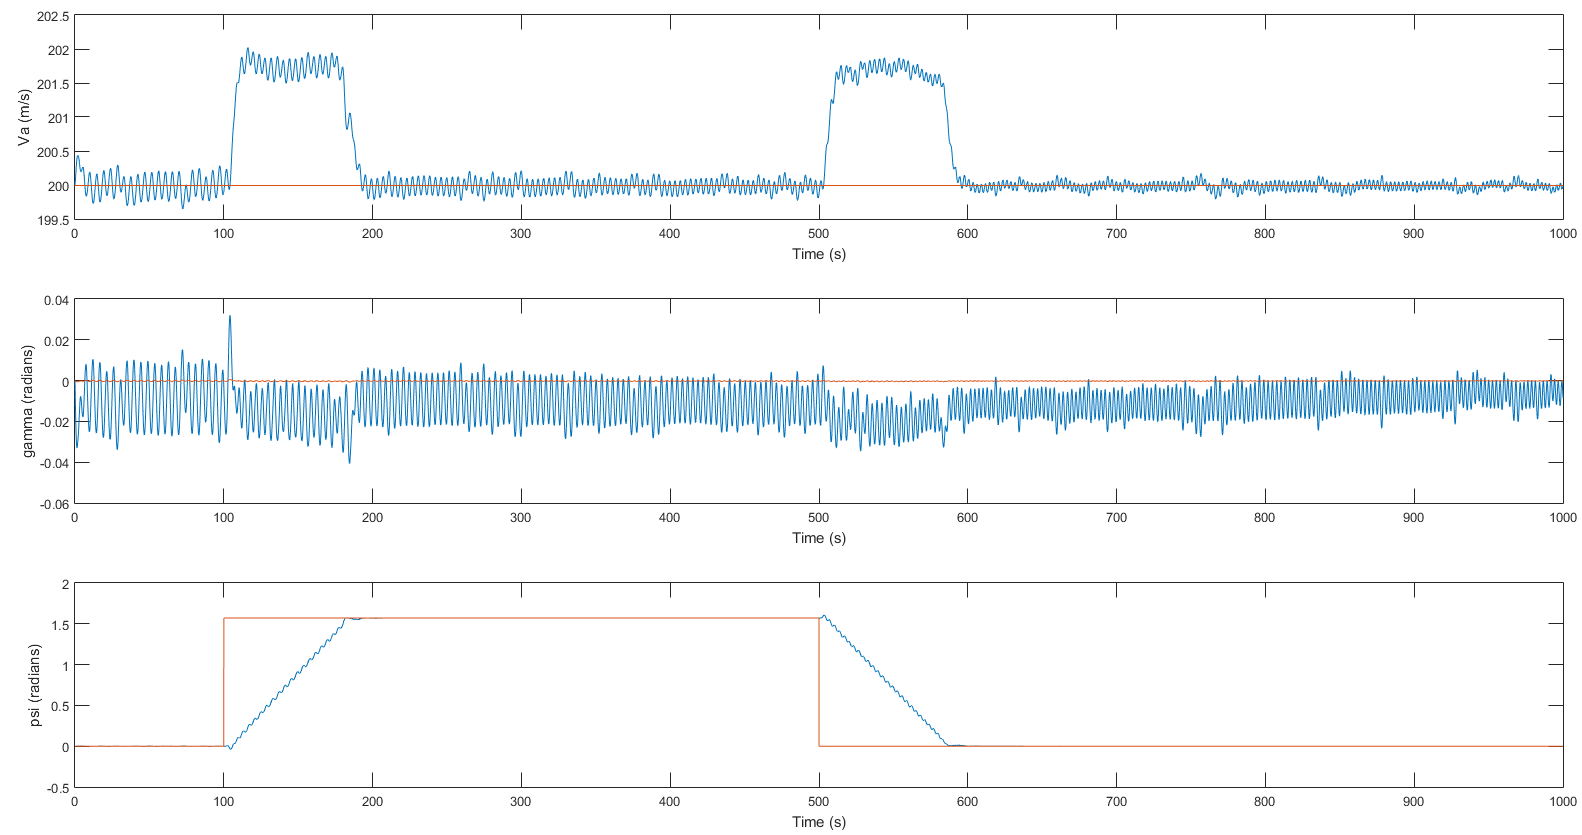
\includegraphics[width=\textwidth]{Figures/Results/ref_zeta_005_NN.png}
\caption[Reference tracking for $\zeta=0.05$ with NN correction]{$V_a$, $\gamma$ and $\psi$ for measured and desired values for $\zeta=0.05$ with NN correction}
\label{fig:ref_zeta_005_NN}
\end{figure}

This first result shows in contrast to the non adaptive control some improvements, mainly when comparing after $t=600s$. Comparing the airspeed, the value $V_a$ remains close to the desired value of $200ms^{-1}$ without reaching greater values as seen previously. Regarding the yaw, besides an expected delay reaching the desired values, the system follows the reference with little to no error, this time without becoming unstable after $t=600s$.

\subsection{System Failures}

\subsubsection{Actuator failure}

\subsubsection{Icing conditions}

\section{Guidance controller}
\label{section:results/guidance_control}


 % file "Thesis_Results.tex"
\cleardoublepage

%%%%%%%%%%%%%%%%%%%%%%%%%%%%%%%%%%%%%%%%%%%%%%%%%%%%%%%%%%%%%%%%%%%%%%%%
%                                                                      %
%     File: Thesis_Conclusions.tex                                     %
%     Tex Master: Thesis.tex                                           %
%                                                                      %
%     Author: Andre C. Marta                                           %
%     Last modified :  2 Jul 2015                                      %
%                                                                      %
%%%%%%%%%%%%%%%%%%%%%%%%%%%%%%%%%%%%%%%%%%%%%%%%%%%%%%%%%%%%%%%%%%%%%%%%

\chapter{Conclusions}
\label{chapter:conclusions}

This final chapter will list the conclusions that can be drawn from chapter \ref{chapter:results}. Reiterating the goals initially established for this work, these were the following

\begin{itemize}
\item \textbf{Design and validate a plane model}
\item \textbf{Implement and test a feedback linearisation controller}
\item \textbf{Adaptively improve control with an Online Neural Network}
\end{itemize}

These goals and the results obtained will be discussed, to finally conclude on the successfulness of the work made. 

% ----------------------------------------------------------------------
\section{Feedback Linearisation Controller}
\label{section:conclusions/fbl_controller}

The first step, before designing and implementing a controller, was to establish the model of a commercial airplane in a numeric simulation environment. The Boeing 737 as used, as information on this aircraft was readily available, simulated in Matlab Simulink. Note that for this work only cruise flight conditions were considered, as the chosen aircraft model was only validated in such conditions. The feedback linearisation controller was also designed having this assumption in mind. 

Assuming cruise conditions, in section \ref{section:results/validation} it was demonstrated the airplane model followed the expected theoretical results. This was made using the FBL controller to make the simulation follow cruise conditions at the required speed. Once this first goal was achieved, it allowed to build the rest of the controller structure around it. 

The nonlinear control law for fast dynamics was then submitted to different types of perturbations and inversion errors. The controller showed to be robust to not only to errors in inertia estimation as well as small system failures. For more serious control perturbations however, the aircraft could not, as would be expected, follow the desired inputs. Using a $99.5\%$ smaller inertia relative to its true value in the NLI algorithm, increasing by $200\%$ the drag coefficient or by heavily reducing the ability of the control surfaces to influence the plane's dynamics, the aircraft's behaviour showed much higher reference tracking errors, sometimes even becoming uncontrollable. Concluding this first section the designed controller, using a model based approach, proved to be robust to most external perturbations and internal errors. 


% ----------------------------------------------------------------------
\section{Online Neural Network}
\label{section:conclusions/online_neural_network}

Once the limitations of the system were known, an online neural network was added to adaptively reduce these limitations for a wide range of perturbations (e.g. actuator failure, icing conditions, etc.). The network was at no point trained previously to the simulation. 

Taking firstly the errors caused by errors in parameter estimations and gain tuning (for the linear law controlling the aircraft's model linearised by the FBL), the network showed improvements in robustness and reduced errors in airspeed and heading following, when compared to the same controller without the network. Similar tests were made with reduced control from actuators and in icing conditions. For the actuator failure case although the network slightly improve heading convergence times, reducing $C_{\delta_{ail}}, C_{\delta_{ele}}, C_{\delta_{rud}}$ by 80\% is still a too big perturbation for a commercial aircraft to recover from. For icing condition were simulated reduced lift coefficient, increased drag and reduced roll control ($C_{\delta_{ail}}$ was reduced by 30\%). For this case however, while the non corrected was unable to follow a heading and flight path angle references, this was not the case once the online neural network was added to the system. Indeed the network allowed the aircraft to follow a sinusoidal heading reference and to reduce the difference between $\gamma$ and its desired value. 

The same network architecture was used for all cases described above. Taking this into account it can be concluded that the goal of designing a neural network that would make the original NLI law more robust and able to adapt to different perturbations was indeed achieved.

% ----------------------------------------------------------------------
\section{Future Work}
\label{section:future}

In this work, the neural network used had a relatively simple architecture of one hidden layer, using both sigmoid and linear activation functions. One way to continue this work is to try different architectures that have been used in other works, such as recurrent neural networks, Radial Basis Function neurons or larger numbers of hidden layer, to improve upon its adaptive capabilities. 

This method was also only used to correct the control of the fast dynamics of a commercial aircraft, and a similar system could be used to adaptively improve its guidance laws. The results obtained however allow to make a commercial aircraft follow 4D trajectories, even in case of external disturbances or system failures. The next step is now to use these trajectories to optimise air traffic management, allowing even several commercial aircraft to travel along these trajectories, reducing the work load of air traffic controllers while increasing the capacity of a given air control zone.

 % file "Thesis_Conclusions.tex"
\cleardoublepage

% ----------------------------------------------------------------------
%  Bibliography
% ----------------------------------------------------------------------

% Add entry in the table of contents as chapter
\phantomsection
\addcontentsline{toc}{chapter}{\bibname}

% Include all references in .bib file, even non-cited ones...
%\nocite{*} % this should be used carefully because it is not correct!

% Produces the bibliography section when processed by BibTeX
%
% Bibliography style
% > entries ordered alphabetically
%\bibliographystyle{plain}
% > unsorted with entries appearing in the order in which the citations appear.
%\bibliographystyle{unsrt}
% > entries ordered alphabetically, with first names and names of journals and months abbreviated
%\bibliographystyle{abbrv}
% > entries ordered alphabetically, with reference markers based on authors' initials and publication year
%\bibliographystyle{alpha}
%
% Replacement bibliography styles provided by 'natbib' package
% (plainnat.bst, abbrvnat.bst, unsrtnat.bst )
% > entries ordered alphabetically
%\bibliographystyle{plainnat}
% > unsorted with entries appearing in the order in which the citations appear.
%\bibliographystyle{unsrtnat}
% > entries ordered alphabetically, with first names and names of journals and months abbreviated
%\bibliographystyle{abbrvnat} % <<<<< SELECT IF USING REFERENCES BY AUTHOR/YEAR
% > entries ordered alphabetically, with reference markers based on authors' initials and publication year
%\bibliographystyle{alpha}
%
% Custom bibliography style adapted from 'natbib' package
%   (based on http://tex.stackexchange.com/questions/5053/is-it-possible-to-get-unsrt-abbrv-bibliography)
%   (unsrtnat.bst + abbrvnat.bst -> abbrvunsrtnat.bst)
%   (original files copied from:
%   http://tug.ctan.org/macros/latex/contrib/natbib/abbrvnat.bst
%   http://tug.ctan.org/macros/latex/contrib/natbib/unsrtnat.bst
% > unsorted with entries appearing in the order in which the citations appear, with first names and names of journals and months abbreviated.
\bibliographystyle{abbrvunsrtnat} % <<<<< SELECT IF USING REFERENCES BY NUMBER (CITATION ORDER)

% External bibliography database file in the BibTeX format
\bibliography{Thesis_bib_DB} % file "Thesis_bib_DB.bib"

\cleardoublepage

% ----------------------------------------------------------------------
%  Appendix (optional)
%
%  CAUTION: 1) the main document (up to the conclusions) shall not exceed 80 pages
%           2) the document shall not exceed a total of 100 pages (per IST regulations)
% ----------------------------------------------------------------------
\appendix

% add page number prefix according to apendix chapter (optional)
%\renewcommand{\thepage}{\thechapter.\arabic{page}}

% re-set arabic numbering (A.1,A.2,...) (optional, use only if chapter prefix is added)
%\setcounter{page}{1}

%%%%%%%%%%%%%%%%%%%%%%%%%%%%%%%%%%%%%%%%%%%%%%%%%%%%%%%%%%%%%%%%%%%%%%%%
%                                                                      %
%     File: Thesis_Appendix_A.tex                                      %
%     Tex Master: Thesis.tex                                           %
%                                                                      %
%     Author: Andre C. Marta                                           %
%     Last modified :  2 Jul 2015                                      %
%                                                                      %
%%%%%%%%%%%%%%%%%%%%%%%%%%%%%%%%%%%%%%%%%%%%%%%%%%%%%%%%%%%%%%%%%%%%%%%%

\chapter{Vector calculus}
\label{chapter:appendixVectors}

In case an appendix if deemed necessary, the document cannot exceed a total of 100 pages...

Some definitions and vector identities are listed in the section below.

% ----------------------------------------------------------------------
\section{Vector identities}
\label{section:vectorIdentities}

\begin{equation}
	\nabla \times \left( \nabla \phi \right) = 0
	\label{eq:cross_nnp}
\end{equation}

\begin{equation}
	\nabla \cdot \left( \nabla \times {\bf u} \right) = 0
	\label{eq:dotCross_nnu}
\end{equation}

 % file "Thesis_Appendix_A.tex"
\cleardoublepage

% re-set arabic numbering (B.1,B.2,...) (optional, use only if chapter prefix is added)
%\setcounter{page}{1}

%%%%%%%%%%%%%%%%%%%%%%%%%%%%%%%%%%%%%%%%%%%%%%%%%%%%%%%%%%%%%%%%%%%%%%%%
%                                                                      %
%     File: Thesis_Appendix_B.tex                                      %
%     Tex Master: Thesis.tex                                           %
%                                                                      %
%     Author: Andre C. Marta                                           %
%     Last modified :  2 Jul 2015                                      %
%                                                                      %
%%%%%%%%%%%%%%%%%%%%%%%%%%%%%%%%%%%%%%%%%%%%%%%%%%%%%%%%%%%%%%%%%%%%%%%%

\chapter{Technical Datasheets}
\label{chapter:appendixDatasheets}

It is possible to add PDF files to the document, such as technical sheets of some equipment used in the work.

% ----------------------------------------------------------------------
\section{Some Datasheet}
\label{section:datasheet}

% See more options to include PDF files in
% http://mirror.unl.edu/ctan/macros/latex/contrib/pdfpages/pdfpages.pdf
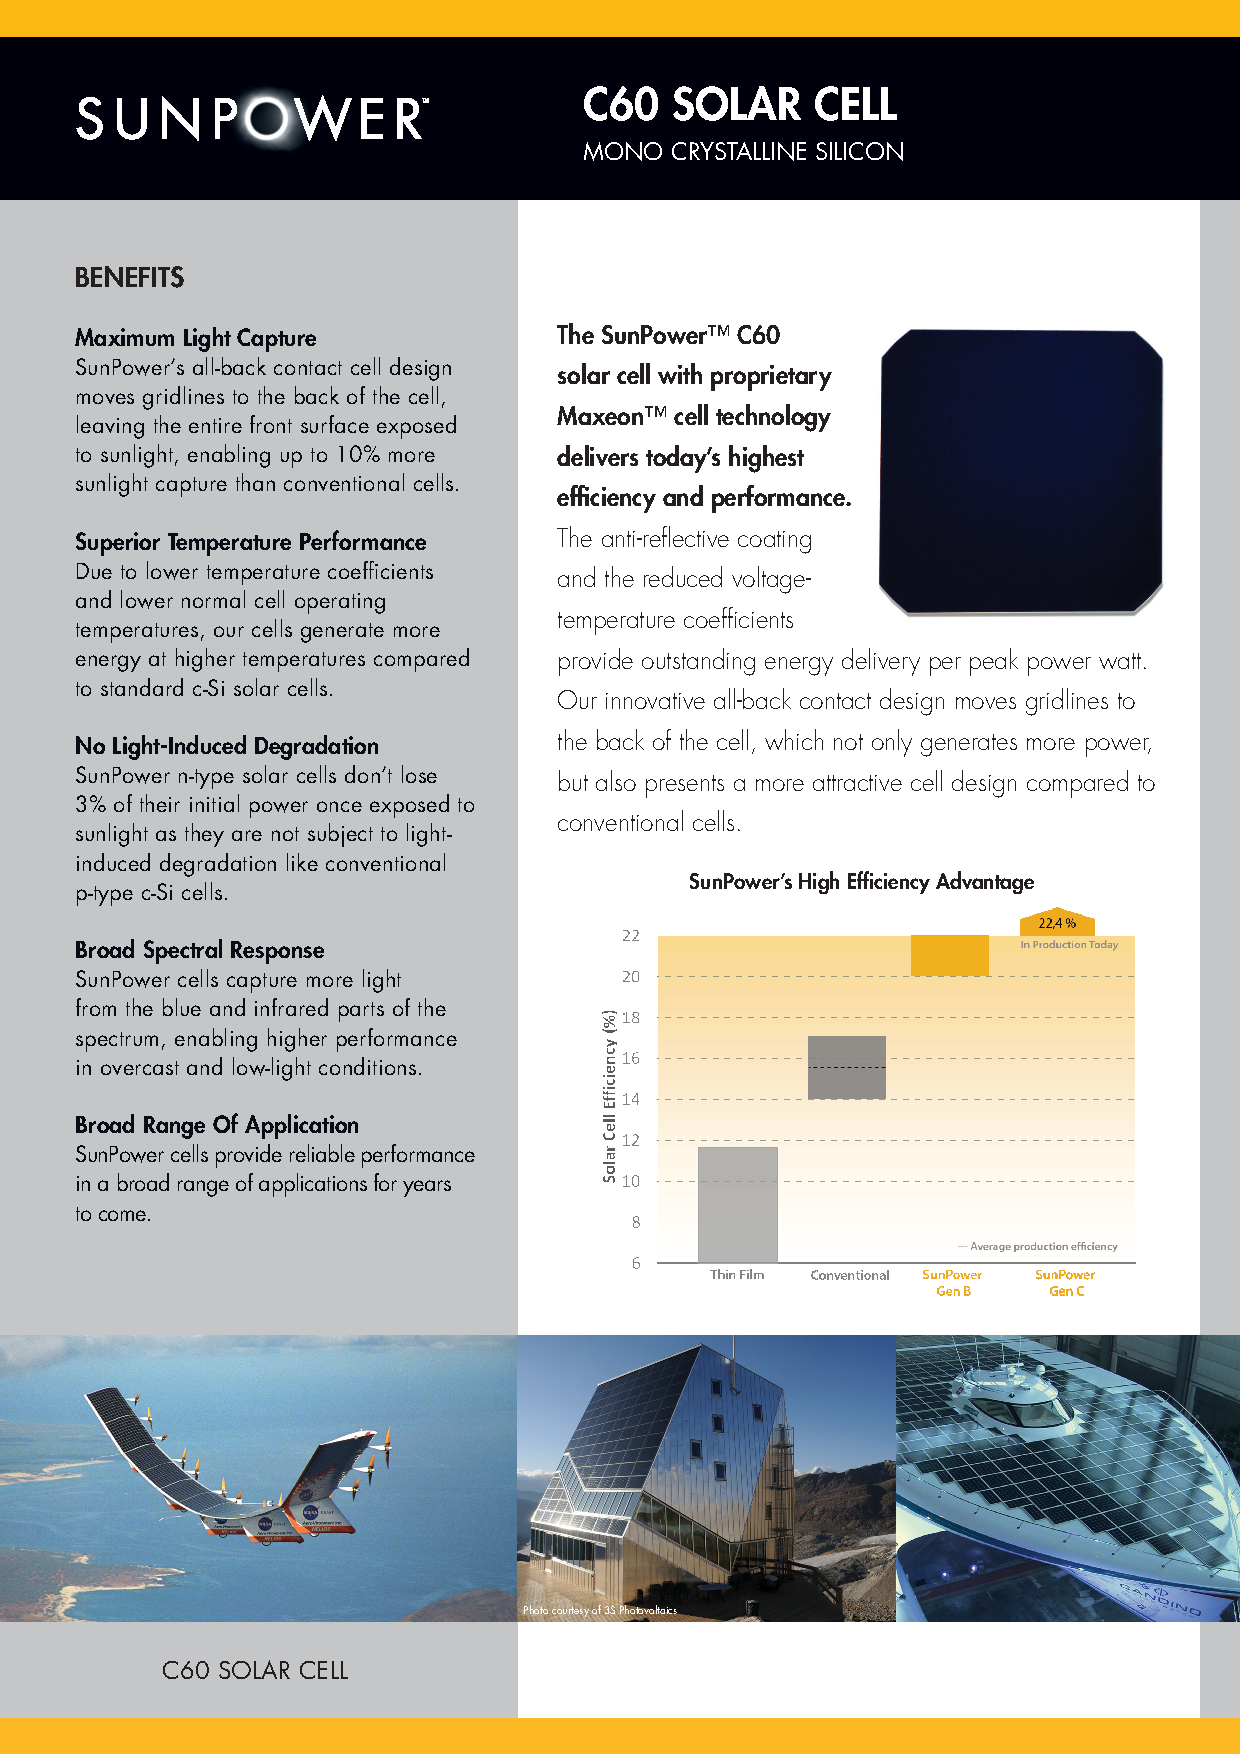
\includepdf[pages={1-2},nup=1x2,landscape=true]{Figures/SolarCell_Sunpower_C60.pdf}

 % file "Thesis_Appendix_B.tex"
\cleardoublepage

% ----------------------------------------------------------------------
\end{document}
% ----------------------------------------------------------------------

